%!TEX TS-program = pdflatex
% dissertation.tex -- main dissertation file
%
% Wisconsin dissertation template
% Copyright (c) 2008-2009 William C. Benton.  All rights reserved.
%
% This program can redistributed and/or modified under the terms
% of the LaTeX Project Public License Distributed from CTAN
% archives in directory macros/latex/base/lppl.txt; either
% version 1 of the License, or (at your option) any later version.
%
% This program includes other software that is licensed under the
% terms of the LPPL and the Perl Artistic License; see README for details.
%
% You, the user, still hold the copyright to any document you produce
% with this software (like your dissertation).
%

%%% You'll want ``oneside'' for the deposit version, but probably not for any versions that don't need to meet the UW requirements
\documentclass[12pt,oneside,letterpaper]{memoir}

% preamble.tex -- packages to include
%
% Wisconsin dissertation template
% Copyright (c) 2008 William C. Benton.  All rights reserved.
%
% This program can redistributed and/or modified under the terms
% of the LaTeX Project Public License Distributed from CTAN
% archives in directory macros/latex/base/lppl.txt; either
% version 1 of the License, or (at your option) any later version.
%
% This program includes other software that is licensed under the
% terms of the LPPL and the Perl Artistic License; see README for details.
%
% You, the user, still hold the copyright to any document you produce
% with this software (like your dissertation).
\usepackage{float}
\usepackage[section]{placeins}
%% You should use natbib
%\
%\IfFileExists{natbib.sty}{%
%\usepackage[sectionbib]{natbib}%
%\usepackage{chapterbib}
%}{}
\usepackage[backend=biber, style=phys]{biblatex}
\bibliography{thesis.bib}
%% You probably need appendix, if you want appendices
\IfFileExists{appendix.sty}{%
\usepackage{appendix}%
}{}

\usepackage{CJKutf8}

%set table of content and numbering depth
\setcounter{tocdepth}{2}
\setcounter{secnumdepth}{3}

%% the spacing in memoir is weird, you'll need to use this
\DisemulatePackage{setspace}
%\usepackage[doublespacing]{setspace}
\usepackage{setspace}

%% geometry package to help with margins on title page
\usepackage{geometry}

%% List setup; the ``hanglist`` environment will allow you to have
%% nicely-typeset enumerated lists (i.e. with the numbers hanging in
%% the margins).  You need at least version 2.1 of enumitem.sty.  If
%% you don't have enumitem installed at all, hanglist will just be an
%% alias for enumerate.
\IfFileExists{enumitem.sty}{%
\usepackage[loadonly]{enumitem}[2007/06/30]%
\newlist{hanglist}{enumerate}{1}% 
\setlist[hanglist]{label=\arabic*.}%
\setlist[hanglist,1]{leftmargin=0pt}%
}{%
\newenvironment{hanglist}{\begin{enumerate}}{\end{enumerate}}%
}

%% Comment out any of these that you don't want
\usepackage{amssymb}
\usepackage{amsmath}
\usepackage{amsthm}
%\usepackage{theorem}
\usepackage{hyperref}

\IfFileExists{mathpartir.sty}{%
\usepackage{mathpartir}%
}{}

%%%%% LISTINGS package and setup
\IfFileExists{listings.sty}{%
\usepackage{listings}%
}{}



%% Get rid of ugly borders around PDF hyperlinks (e.g. for cross-references, bib entries, or URLs)
\hypersetup{pdfborder = 0 0 0}

%% You want microtype.
\IfFileExists{microtype.sty}{%
\usepackage[protrusion=true,expansion=true]{microtype}%
}{}

%\pagestyle{thesisdraft}

% Surround parts of graphics with box
\usepackage{boxedminipage}

%% booktabs (thx to Nate Rosenblum for bringing this beautiful package
%% to my attention)
\IfFileExists{booktabs.sty}{%
\usepackage{booktabs}%
}{}

% This is now the recommended way for checking for PDFLaTeX:
\usepackage{ifpdf}

%% Avoid ugly "Type 3" fonts
\usepackage{lmodern}
\usepackage[LY1]{fontenc}

%% Substitute your favorite serif and sans fonts here....
\IfFileExists{tgpagella.sty}{%
% TeX Gyre pagella, like Palatino
\usepackage{tgpagella}%
}{}

\usepackage[LY1]{eulervm}

\ifpdf
\usepackage[pdftex]{graphicx}
\else
\usepackage{graphicx}
\fi

\usepackage{makeidx}
\makeindex

{\theoremstyle{plain}
\newtheorem{thm}{Theorem}[chapter]
\newtheorem{cor}[thm]{Corollary}
\newtheorem{define}[thm]{Definition}
\newtheorem{exmpl}[thm]{Example}
}
{\theoremstyle{remark}
\newtheorem{rmk}[thm]{Remark}
}

\newtheoremstyle{customsty1}
{3pt}%
{3pt}%
{}% --- body font
{}% --- indent amount
{\bfseries}% --- Theorem head font
{:}% --- Punctuation after head
{.5em}% --- space after head
{}% --- theorem head spec (can be left empty, meaning 'normal')

% Define 'newtheorems' that use ``customsty1''
{\theoremstyle{customsty1} 
}


%%% NB: the ``deposit'' chapter- and page- styles should conform to UW
%%% requirements.  If you are producing a pretty version of your
%%% dissertation for web use later, you will certainly want to make
%%% your own chapter and page styles.

\makechapterstyle{deposit}{%
  \renewcommand{\chapterheadstart}{}
  \renewcommand{\printchaptername}{}
  \renewcommand{\chapternamenum}{}
  \renewcommand{\printchapternum}{\parbox{2em}{\MakeLowercase{\Large\scshape\thechapter{}}} }
  \renewcommand{\afterchapternum}{}
  \renewcommand{\printchaptertitle}[1]{%
  \raggedright\Large\scshape\MakeLowercase{##1}}
  \renewcommand{\afterchaptertitle}{%
  \vskip\onelineskip \hrule\vskip\onelineskip}
}

\makepagestyle{deposit}
 
\makeatletter
 
\renewcommand{\chaptermark}[1]{\markboth{#1}{}}
\renewcommand{\sectionmark}[1]{\markboth{#1}{}}
 
\makeevenfoot{deposit}{}{}{}
\makeoddfoot{deposit}{}{}{}
\makeevenhead{deposit}{\thepage}{}{}
\makeoddhead{deposit}{}{}{\thepage}
\makeatother

%%% set up page numbering for chapter pages to satisfy UW requirements
%%% NB: You will want to delete until the ``SNIP'' mark if you are
%%% making a ``nice'' copy
\copypagestyle{chapter}{plain}
\makeoddfoot{chapter}{}{}{}
\makeevenhead{chapter}{\thepage}{}{}
\makeoddhead{chapter}{}{}{\thepage}
%%% SNIP

%%% bib nonsense
\makeatletter
\newenvironment{wb-bib}[1]{%
  \chapter*{references}
\ifnobibintoc\else 
\phantomsection 
%\addcontentsline{toc}{chapter}{References} 
\fi 
\prebibhook
  \begin{bibitemlist}{#1}}{\end{bibitemlist}\postbibhook}

\AtBeginDocument{%
  \@ifpackageloaded{natbib}{% natbib is loaded
    \addtodef{\endthebibliography}{}{\vskip-\lastskip\postbibhook}
    \@ifpackagewith{natbib}{sectionbib}{% with sectionbib option
      \renewcommand{\bibsection}{\@memb@bsec}}%
      {\renewcommand{\bibsection}{\@memb@bchap}}}%
  {}
  \@ifpackagewith{chapterbib}{sectionbib}{%
    \renewcommand{\sectionbib}[2]{}
    \renewcommand{\bibsection}{\@memb@bsec}}{}
}
\makeatother

% defs.tex -- wbepi environment for chapter epigraphs and other useful defs.
%
% Wisconsin dissertation template
% Copyright (c) 2008 William C. Benton.  All rights reserved.
%
% This program can redistributed and/or modified under the terms
% of the LaTeX Project Public License Distributed from CTAN
% archives in directory macros/latex/base/lppl.txt; either
% version 1 of the License, or (at your option) any later version.
%
% This program includes other software that is licensed under the
% terms of the LPPL and the Perl Artistic License; see README for details.
%
% You, the user, still hold the copyright to any document you produce
% with this software (like your dissertation).


%% put lstnewenvironment declarations here, if you're using listings

%% end lstnewenvironment declarations

%% I put convenience definitions that will go in several chapters here

%%%%% begin convenience definitions

\makeatletter
\newcommand{\wb@episource}{}
\newenvironment{wbepi}[1]{\begin{quote}\renewcommand{\wb@episource}{#1}\itshape}{\par\upshape \raggedleft --- \textsc{\wb@episource}\\ \end{quote}}
\makeatother

%%%%% SVN
\IfFileExists{svn-multi.sty}{%
\usepackage{svn-multi}%
%%% Uncomment the second one and comment out the first one if you want
%%% to include subversion revision information in each file.
\newcommand{\vcinfo}{}%
%\newcommand{\vcinfo}{\begin{centering}\fbox{\fbox{\parbox{5in}{Author: \svnauthor\\Revision: \svnfilerev\\Last changed on: \svnfiledate\\URL: \svnkw{HeadURL}}}}\\[1em]\end{centering}}%
}{%
\newcommand{\svnidlong}[4]{}%
\newcommand{\svnfilerev}{}%
\newcommand{\svnauthor}{}%
\newcommand{\svnfiledate}{}%
\newcommand{\svnkw}{}%
\newcommand{\vcinfo}{}%
}

%%%%% end convenience definitions

% thesisdefs.tex

% This is mostly adapted from withesis.cls.  The original copyright
% notice for withesis.cls follows, preceded by two percent signs (%%):

%% withesis.cls
%% LaTeX Style file for the University of Wisconsin-Madison Thesis Format
%% Adapted from the Purdue University Thesis Format
%% Originally by Dave Kraynie
%% Edits by Darrell McCauley
%% Adapted to UW-Madison format by Eric Benedict  (Noted with <EB>)
%% Updated to LaTeX2e by Eric Benedict 24 July 00
%% 
%%=============================================================================
%% Licensed under the Perl Artistic License.
%% see: http://www.ctan.org/tex-archive/help/Catalogue/licenses.artistic.html
%% for more info...
%%=============================================================================

% withesis.cls is available from CTAN.  The modifications to this file
% are also licensed under the Perl Artistic License.

% --wb, 2008

\makeatletter

\newcounter {tocpage}
\newcounter {lofpage}
\newcounter {lotpage}
\newcounter {listofheading}

\newcommand\@thesistitlemedskip{0.25in}
\newcommand\@thesistitlebigskip{0.55in}
%\newcommand{\degree}[1]{\gdef\@degree{#1}}
\newcommand{\project}{\gdef\@doctype{A masters project report}}
\newcommand{\prelim}{\gdef\@doctype{A preliminary report}}
\newcommand{\thesis}{\gdef\@doctype{A thesis}}
\newcommand{\dissertation}{\gdef\@doctype{A dissertation}}
\newcommand{\department}[1]{\gdef\@department{(#1)}}
\newcommand{\oralexamdate}[1]{\gdef\@oralexamdate{#1}} 
\newcommand{\committeeone}[1]{\gdef\@committeeone{#1}}
\newcommand{\committeetwo}[1]{\gdef\@committeetwo{#1}}
\newcommand{\committeethree}[1]{\gdef\@committeethree{#1}}
\newcommand{\committeefour}[1]{\gdef\@committeefour{#1}}
\newcommand{\committeefive}[1]{\gdef\@committeefive{#1}}
\newcommand{\committeesix}[1]{\gdef\@committeesix{#1}}
\newcommand{\committeeseven}[1]{\gdef\@committeeseven{#1}}

\newenvironment{titlepage}
 {\@restonecolfalse\if@twocolumn\@restonecoltrue\onecolumn
  \else \newpage \fi \thispagestyle{empty}
% \c@page\z@ -- deleted: count title page in thesis
}{\if@restonecol\twocolumn \else \newpage \fi}

\gdef\@degree{Doctor of Philosophy}    %Default is PhD
\gdef\@doctype{A dissertation}         %Default is dissertation

\gdef\@department{(Physics)} % Default is Electical Engineering
\gdef\@oralexamdate{}
\gdef\@committeeone{}
\gdef\@committeetwo{}
\gdef\@committeethree{}
\gdef\@committeefour{}
\gdef\@committeefive{}
\gdef\@committeesix{}
\gdef\@committeeseven{}



\renewcommand{\maketitle}{%
  \begin{titlepage}
%-----------------------------------------------------------------------------
% -- The thesis office doesn't like thanks on title page.  Put it in
% -- the acknowledgments.  This is here so you don't have to change
% -- your titlepage when converting from report style. -> from Purdue, but I
%        left it here since it seems compatible with UW-Madison, Eric
%-----------------------------------------------------------------------------
    \def\thanks##1{\typeout{Warning: `thanks' deleted from thesis titlepage.}}
    \let\footnotesize\small \let\footnoterule\relax \setcounter{page}{1}
 %sets new margins for title page so that committee members can be placed there

   % \vspace*{0.1in}
    \begin{center}
      {\textbf{\expandafter\uppercase\expandafter{\@title}}} \\[\@thesistitlebigskip]
       by \\[\@thesistitlemedskip]
      \@author \\[\@thesistitlebigskip]
      \@doctype\ submitted in partial fulfillment of \\
      the requirements for the degree of\\[\@thesistitlebigskip]
      \@degree \\[\@thesistitlemedskip]
      \@department \\[\@thesistitlebigskip]
      at the \\[\@thesistitlebigskip]
      UNIVERSITY OF WISCONSIN--MADISON\\[\@thesistitlebigskip]
      \@date \\[\@thesistitlebigskip]
    \end{center}
% section added by Steven Baumgart on 3/2012
% adds committee list to the title page
% add or delete committee members as you need to, these are defined in the dissertation.tex document 
% comment out other things as you need to as well. - SB

\noindent Date of final oral examination: \@oralexamdate \hspace*{\fill} \\[\@thesistitlemedskip]
\noindent The dissertation is approved by the following members of the Final Oral Committee:\\*
\indent \@committeeone\\*
\indent \@committeetwo\\*
\indent \@committeethree\\*
\indent \@committeefour\\*
\indent \@committeefive
%\indent \@committeesix\\* %if you uncomment any of these you the last line needs to have no line break ``//*``
%\indent \@committeeseven


  \end{titlepage}

  \setcounter{footnote}{0}
  \setcounter{page}{1} %title page is NOT counted
  \let\thanks\relax
  \let\maketitle\relax  \let\project\relax \let\prelim\relax %\let\degree\relax
  \let\department\relax
  \gdef\@thanks{}\gdef\@degree{}\gdef\@doctype{}
  \gdef\@department{}
  %\gdef\@author{}\gdef\@title{}
}


%=============================================================================
% ABSTRACT
%=============================================================================
% The abstract should begin with two single-spaced lines describing
% the author and title in a standard format.  After these lines comes
% the standard abstract.
%=============================================================================
\def\abstract{
  \chapter*{Abstract}
  \addcontentsline{toc}{chapter}{Abstract}
  \relax\markboth{Abstract}{Abstract}}
\def\endabstract{\par\newpage}


%=============================================================================
% UMI ABSTRACT
%=============================================================================
% The UMI abstract should begin with the author and title in a standard format.
% After the author comes the advisor and university. After these lines comes
% a bunch of double spaced text to make up the standard abstract.
% After the abstract, the advisor's approval signature follows.
% This page is not numbered and is delivered seperately to the thesis office.
%=============================================================================

\def\advisortitle#1{\gdef\@advisortitle{#1}}
\def\advisorname#1{\gdef\@advisorname{#1}}
\gdef\@advisortitle{Professor}
\gdef\@advisorname{Daniel Den Hartog}

\def\umiabstract{
             \thispagestyle{empty}
                  \addtocounter{page}{-1}
                \begin{center}
                  {\textbf{\expandafter\uppercase\expandafter{\@title}}}\\
                  \vspace{12pt}
                  \@author \\
                  \vspace{12pt}
                  Under the supervision of \@advisortitle\ \@advisorname\\
                  At the University of Wisconsin-Madison
                \end{center}
}

\def\endumiabstract{\vfill \hfill\@advisorname\par\newpage}


%============================================================================
% VERBATIMFILE
%============================================================================
% \verbatimfile{<filename>}    for verbatim inclusion of a file
% - Note that the precise layout of line breaks in this file is important!
% - added the \singlespace - EB
%============================================================================
\def\verbatimfile#1{\begingroup \singlespace
                    \@verbatim \frenchspacing \@vobeyspaces
                    \input#1 \endgroup
}


%=============================================================================
% SEPARATOR Pages
%   Creates a blank page with a text centered horizontally and vertically.
%   The page is neither counted nor numbered.
%   These pages are required in the thesis format before sections such
%   as appendices, vita, bibliography, etc.
%=============================================================================
\def\separatorpage#1{
  \newpage
  \thispagestyle{empty}
  \addtocounter{page}{-1}
  \null
  \vfil\vfil
  \begin{center}
    {\textbf{#1}}
  \end{center}
  \vfil\vfil
  \newpage}


%=============================================================================
% COPYRIGHTPAGE
%=============================================================================
% The copyright must do the following:
% - start a new page with no number
% - place the copyright text centered at the bottom.
%=============================================================================
\def\copyrightpage{
  \newpage
  \thispagestyle{empty}    % No page number
  \addtocounter{page}{-1}
  \chapter*{}            % Required for \vfill to work
  \begin{center}
   \vfill
   \copyright\ Copyright by \@author\ \@date\\
   All Rights Reserved
  \end{center}}


%=============================================================================
% GLOSSARY
%=============================================================================
% The glossary environment must do the following:
% - produce the table of contents entry for the glossary
% - start a new page with GLOSSARY centered two inches from the top
%=============================================================================
\def\glossary{
  \chapter*{GLOSSARY}
  \addcontentsline{toc}{chapter}{Glossary}}
\def\endglossary{\par\newpage}

%=============================================================================
% NOMENCLATURE
%=============================================================================
% The nomenclature environment must do the following:
% - produce the table of contents entry for the nomenclature section
% - start a new page with NOMENCLATURE centered two inches from the top
%=============================================================================
\def\nomenclature{\separatorpage{DISCARD THIS PAGE}
  \chapter*{Nomenclature}
  \addcontentsline{toc}{chapter}{NOMENCLATURE}}
\def\endnomenclature{\par\newpage}

%=============================================================================
% CONVENTIONS
%=============================================================================
% The conventions environment must do the following:
% - produce the table of contents entry for the nomenclature section
% - start a new page with CONVENTIONS centered two inches from the top
%=============================================================================
\def\conventions{\separatorpage{DISCARD THIS PAGE}
  \chapter*{Conventions}
  \addcontentsline{toc}{chapter}{CONVENTIONS}}
\def\endconventions{\par\newpage}


%=============================================================================
% COLOPHON
%=============================================================================
% The colophon environment must do the following:
% - produce the table of contents entry for the nomenclature section
% - start a new page with COLOPHON centered two inches from the top
%=============================================================================
\def\colophon{\separatorpage{DISCARD THIS PAGE}
  \chapter*{Colophon}
  \addcontentsline{toc}{chapter}{Colophon}}
\def\endcolophon{\par\newpage}

%=============================================================================
% LIST OF SYMBOLS
%=============================================================================
% The list of symbols environment must do the following:
% - produce the table of contents entry for the list of symbols section
% - start a new page with LIST OF SYMBOLS centered two inches from the top
%=============================================================================
\def\listofsymbols{\separatorpage{DISCARD THIS PAGE}
  \eject
  \chapter*{LIST OF SYMBOLS}
  \addcontentsline{toc}{chapter}{LIST OF SYMBOLS}}
\def\endlistofsymbols{\par\newpage}

%=============================================================================
% VITA
%=============================================================================
% The vita environment must do the following:
% - produce a separator page with the word vita centered
% - produce the table of contents entry for the vita
% - start a new page with VITA centered two inches from the top
%=============================================================================
\def\vita{
%  \separatorpage{VITA}         % UW doesn't require this EB
  \chapter*{VITA}
  \addcontentsline{toc}{chapter}{VITA}}
\def\endvita{\par\newpage}

%=============================================================================
% ACKNOWLEDGMENTS
%=============================================================================
% The acknowledgments environment must do the following:
% - start a new page with ACKNOWLEDGMENTS centered two inches from the top
%=============================================================================
\def\acks{
  \chapter*{Acknowledgments}
}
\def\endacks{\par\newpage}

%=============================================================================
% DEDICATION
%=============================================================================
% The dedication environment must do the following:
% - start a new page
% - center the text vertically
% - include the text in a center environment
%=============================================================================
\def\dedication{
  \newpage
  \chapter*{}
  \null\vfil
  \begin{center}}
\def\enddedication{\end{center}\par\vfil\newpage}

%=============================================================================
% DATE
%=============================================================================
%\def\today{\ifcase\month\or
  %January\or February\or March\or April\or May\or June\or
  %July\or August\or September\or October\or November\or December\fi
  %\space\number\day, \number\year}
\newcount\@testday
\def\today{\@testday=\day
  \ifnum\@testday>30 \advance\@testday by -30
  \else\ifnum\@testday>20 \advance\@testday by -20
  \fi\fi
  \number\day\ \
  \ifcase\month\or
    January \or February \or March \or April \or May \or June \or
    July \or August \or September \or October \or November \or December
    \fi\ \number\year
}


%  Single counter for theorems and theorem-like environments:
\newtheorem{theorem}{Theorem}[chapter]
\newtheorem{assertion}[theorem]{Assertion}
\newtheorem{claim}[theorem]{Claim}
\newtheorem{conjecture}[theorem]{Conjecture}
\newtheorem{corollary}[theorem]{Corollary}
\newtheorem{definition}[theorem]{Definition}
\newtheorem{example}[theorem]{Example}
\newtheorem{figger}[theorem]{Figure}
\newtheorem{lemma}[theorem]{Lemma}
\newtheorem{prop}[theorem]{Proposition}
\newtheorem{remark}[theorem]{Remark}

%=============================================================================
% TABLE OF CONTENTS; LIST OF FIGURES; LIST OF TABLES
%=============================================================================
% In report style, \tableofcontents, \listoffigures, etc. are always
% set in single-column style.  @restonecol is used to keep track of
% whether we need to switch back to double column style after the toc.
%
% The only known problem now is that the first page with the new
% layout is too long.  The problem seems to be that the change to
% textheight doesn't take place on the first page.  Even if it's the
% first line in the table of contents macro.  Presumably the same
% problem also occurs in the lof and lot.
%
% I'm taking a shot at fixing the problem by dropping in a throw-away
% page between the change to the height parameters and the start of
% the chapter.  Isn't elegance wonderful?
%
%=============================================================================

%\def\@tableof#1#2#3#4#5{
%{ % limit scope of following declarations!!
%   \@restonecolfalse\if@twocolumn\@restonecoltrue\onecolumn\fi
%   \addtolength{\textheight}{-40pt}       % -24-16
%   %\addtolength{\majorheadskip}{-40pt}    % -24-16
%   \addtolength{\headheight}{52pt}        %  36+16
%   \addtolength{\headsep}{-12pt}          % -12
%   \separatorpage{DISCARD THIS PAGE}
%   \chapter*{#1}
%   #5
%   \relax\markboth{#1}{#1}
%   \hbox to \hsize{#2 \hfil Page}
%   \singlespace
%   \setcounter{#3}{0}
%   \setcounter{listofheading}{1}  % change from 0 to 1 by mccauley, 14may93
%   \def\@oddhead{\vbox to \headheight{\vspace{4pt}
%     \hbox to \hsize{\hfil\textrm{\thepage}} \vfil
%     \ifnum\value{#3}=1
%       \ifnum\value{listofheading}=2
%         \hbox to \hsize{Appendix\hfil} \vspace{4pt} \fi
%       \ifnum\value{listofheading}=1
%         \stepcounter{listofheading} \fi
%       \hbox to \hsize{#2 \hfil Page}
%     \else
%       \setcounter{#3}{1}
%     \fi}}
%   \def\@evenhead{\vbox to \headheight{\vspace{4pt}
%     \hbox to \hsize{\textrm{\thepage}\hfil} \vfil
%     \ifnum\value{#3}=1
%       \ifnum\value{listofheading}=2
%         \hbox to \hsize{Appendix\hfil} \vspace{4pt} \fi
%       \ifnum\value{listofheading}=1
%         \stepcounter{listofheading} \fi
%       \hbox to \hsize{#2 \hfil Page}
%     \else
%       \setcounter{#3}{1}
%     \fi}}
%   \@starttoc{#4}  \if@restonecol\twocolumn\fi
%   \newpage
% }}

% \def\tableofcontents{\@tableof{TABLE OF CONTENTS}{}{tocpage}{toc}{}}
 
% \def\listoffigures{
%   \@tableof{LIST OF FIGURES}{Figure}{lofpage}{lof}
%   {\protect\addcontentsline{toc}{chapter}{LIST OF FIGURES}}}
 
% \def\listoftables{
%   \@tableof{LIST OF TABLES}{Table}{lotpage}{lot}
%   {\protect\addcontentsline{toc}{chapter}{LIST OF TABLES}}}

%=============================================================================
% BIBLIOGRAPHY
%=============================================================================
% The thebibliography environment executes the following commands:
%
%  o start a new 'chapter' with BIBLIOGRAPHY as the heading
%  o produce a separator page for the bibliography
%
%  \def\newblock{\hskip .11em plus .33em minus -.07em} --
%      Defines the `closed' format, where the blocks (major units of
%      information) of an entry run together.
%
%  \sloppy  -- Used because it's rather hard to do line breaks in
%      bibliographies,
%
%  \sfcode`\.=1000\relax --
%      Causes a `.' (period) not to produce an end-of-sentence space.
%=============================================================================
% \altbibtitle
%   The default title for the References chapter is ``LIST OF REFERENCES''
%   Since some people prefer ``BIBLIOGRAPHY'', the command
%   \altbibtitle has been added to change the chapter title.
%   This command does nothing more than change REFERENCES to BIBLIOGRAPHY
%============================================================================
\def\@bibchaptitle{Bibliography}
\def\altbibtitle{\def\@bibchaptitle{Bibliography}}
\def\thebibliography#1{
  %\separatorpage{\@bibchaptitle}
  \global\@bibpresenttrue
  \section*{\@bibchaptitle\markboth{\@bibchaptitle}{\@bibchaptitle}}-
  \addcontentsline{toc}{section}{\@bibchaptitle}
  \vspace{0.375in}    % added to match 4 line requirement
  \interlinepenalty=10000 % added to prevent breaking of bib entries
  \singlespace\list
  {[\arabic{enumi}]}{\settowidth\labelwidth{[#1]}\leftmargin\labelwidth
    \advance\leftmargin\labelsep \usecounter{enumi}}
  \def\newblock{\hskip .11em plus .33em minus -.07em}
  \sloppy
  \sfcode`\.=1000\relax}
\let\endthebibliography=\endlist



\makeatother


%\svnidlong{$LastChangedBy$}{$LastChangedRevision$}{$LastChangedDate$

\setlrmarginsandblock{1in}{1in}{*}
\checkandfixthelayout 
\clearpage\pagenumbering{roman}  % This makes the page numbers Roman (i, ii, etc)

\title{Ion thermal transport and heating in tearing suppressed RFP plasmas}
\author{Zichuan Anthony Xing}
\department{Physics}
\oralexamdate{12/15/2018}
\committeeone{Daniel J. Den Hartog}
\committeetwo{Mark D. Nornberg}
\committeethree{John S. Sarff}
\committeefour{Carl Sovenic}
\committeefive{Paul Terry}

\date{2019}

\begin{document}

%%% Uncomment the following if your .bib contains references that you will not 
%%% explicitly cite, but that should be in the final bibliography:
% \nocite{*}


\DeclareGraphicsExtensions{.pdf, .jpg, .JPG, .tif .png, .PNG, .eps}

\onehalfspace
\newgeometry{left=1in,right=1in,bottom=1in,top=1in}
\maketitle
\restoregeometry %sets the margins back to normal
\doublespace

%% Add \part declarations if you want, but it's not necessary
%\part{Preliminaries}

%%% SOME OF THIS CODE IS ADAPTED FROM THE VENERABLE withesis.cls

% COPYRIGHT PAGE
%  - To include a copyright page use \copyrightpage
\copyrightpage
% ABSTRACT

\begin{abstract}
  
Ion thermal transport in improved confinement plasmas in the Madison Symmetric Torus (MST), a reversed field pinch experiment, is characterized using a model and compare approach. MST can achieve a improved confinement state by reducing tearing mode fluctuations via pulsed parallel current drive (PPCD). An 1-D model is built to foreword model and predict the evolution of $T_i$ profile during PPCD from plasma parameters and an initial condition, and the result is compared to measurements. The model account for classical transport mechanisms, neutral and charge change effects, and ion flow and compression effects, and its predictions is found to match observations in the core. An \adhoc heating term localized near the reversal surface is needed to fully match observations there. As part of the model construction and analysis, the neutral dynamics in PPCD plasmas are investigated using Monte Carlo modeling via the DEGAS2 code. Detailed characterization of neutral density, temperature, ionization rate and charge exchange loss are obtained as well as their evolution during PPCD. The core neutral are calculated to be several hundred eVs in temperature and this contributes to a hollow charge exchange loss profile and partial recovery of lost energy via ionization of hot neutrals. Evidence of inward particle flux in the core during the early PPCD, likely associated with \ecb pinch are also observed during modeling, and the compressional effects from this \ecb are incorporated into the ion thermal transport model. Finally, the location and extent of the needed \adhoc heating is discussed as well as possible contributing physical mechanisms.

Tearing mode reduction during PPCD are sometimes interrupted by brief and limited excitation's know as m = 0 bursts before returning to quiescence. These burst are observed with sudden radially localized impurity heating near the reversal surface followed by equilibration to previous temperature. Despite strong toroidal localization of the burst fluctuations, the heating does not exhibit toroidal time delay that would be associated with heat transport, pointing to the likelihood of wave or turbulence based heating. Possible anisotropy in heating is investigates and found inconclusive, and the equilibration is found to be faster than what would be expected for the majority ion based on the aforementioned model, possibly indicating that majority heating response is significantly different than the impurity response.

\end{abstract}
%\begin{umiabstract}
%  
Ion thermal transport in improved confinement plasmas in the Madison Symmetric Torus (MST), a reversed field pinch experiment, is characterized using a model and compare approach. MST can achieve a improved confinement state by reducing tearing mode fluctuations via pulsed parallel current drive (PPCD). An 1-D model is built to foreword model and predict the evolution of $T_i$ profile during PPCD from plasma parameters and an initial condition, and the result is compared to measurements. The model account for classical transport mechanisms, neutral and charge change effects, and ion flow and compression effects, and its predictions is found to match observations in the core. An \adhoc heating term localized near the reversal surface is needed to fully match observations there. As part of the model construction and analysis, the neutral dynamics in PPCD plasmas are investigated using Monte Carlo modeling via the DEGAS2 code. Detailed characterization of neutral density, temperature, ionization rate and charge exchange loss are obtained as well as their evolution during PPCD. The core neutral are calculated to be several hundred eVs in temperature and this contributes to a hollow charge exchange loss profile and partial recovery of lost energy via ionization of hot neutrals. Evidence of inward particle flux in the core during the early PPCD, likely associated with \ecb pinch are also observed during modeling, and the compressional effects from this \ecb are incorporated into the ion thermal transport model. Finally, the location and extent of the needed \adhoc heating is discussed as well as possible contributing physical mechanisms.

Tearing mode reduction during PPCD are sometimes interrupted by brief and limited excitation's know as m = 0 bursts before returning to quiescence. These burst are observed with sudden radially localized impurity heating near the reversal surface followed by equilibration to previous temperature. Despite strong toroidal localization of the burst fluctuations, the heating does not exhibit toroidal time delay that would be associated with heat transport, pointing to the likelihood of wave or turbulence based heating. Possible anisotropy in heating is investigates and found inconclusive, and the equilibration is found to be faster than what would be expected for the majority ion based on the aforementioned model, possibly indicating that majority heating response is significantly different than the impurity response.

%\end{umiabstract}


%% BEGIN PAGESTYLE

%%% You can pick a pagestyle if you want; see the memoir class
%%% documentation for more info.  The default ``deposit'' option meets
%%% the UW thesis typesetting requirements but is probably
%%% unsatisfactory for making a version of your dissertation that
%%% won't be deposited to the graduate school (e.g. for web or a nice
%%% printed copy)

%\chapterstyle{deposit}
%\pagestyle{deposit}


% ACKNOWLEDGMENTS
\begin{acks}
\begin{CJK*}{UTF8}{gbsn}

This work would not have been possible with out the support and insight of an astoundingly large number of people. Starting with my parents 杏子穿       But mostly me; I worked hard. Go me!

\clearpage\end{CJK*}
\end{acks}

% DEDICATION
\begin{dedication}
	\emph{In memory of\bigskip \\Michael Rust-Smith\\(May 9th, 2010)\bigskip \\Shannon S. Jones\\(November 27th, 2014)\bigskip \\and\\Nebiyou Tulu\\(March 25th, 2015)}
\end{dedication}
% CONTENTS, TABLES, FIGURES
%\renewcommand{\printtoctitle}[1]{\chapter*{#1}}
%\renewcommand{\printloftitle}[1]{\chapter*{#1}}
%\renewcommand{\printlottitle}[1]{\chapter*{#1}}

%\renewcommand{\tocmark}{}
%\renewcommand{\lofmark}{}
%\renewcommand{\lotmark}{}

%\renewcommand{\tocheadstart}{}
%\renewcommand{\lofheadstart}{}
%\renewcommand{\lotheadstart}{}

%\renewcommand{\aftertoctitle}{}
%\renewcommand{\afterloftitle}{}
%\renewcommand{\afterlottitle}{}

%\renewcommand{\cftchapterfont}{\normalfont} 
%\renewcommand{\cftsectionfont}{\itshape} 
%\renewcommand{\cftchapterpagefont}{\normalfont} 
%\renewcommand{\cftchapterpresnum}{\bfseries} 
%\renewcommand{\cftchapterleader}{} 
%\renewcommand{\cftsectionleader}{} 
%\renewcommand{\cftchapterafterpnum}{\cftparfillskip} 
%\renewcommand{\cftsectionafterpnum}{\cftparfillskip} 

% \captionnamefont{\small\sffamily} 
% \captiontitlefont{\small\sffamily} 

\defbibheading{bibliography}[\bibname]{%
\pagebreak
\section{#1}%
\markboth{#1}{#1}}

%%% no extra space before the entry, or in the LoF/LoT
\setlength{\cftbeforechapterskip}{0pt plus 0pt}
%\renewcommand*{\insertchapterspace}{}


% \renewcommand{\listfigurename}{list of figures}
% \renewcommand{\listtablename}{list of tables}
\renewcommand{\contentsname}{Table of Contents}
\renewcommand*{\cftchapterleader}{\cftchapterfont\cftdotfill{\cftchapterdotsep}}
\renewcommand*{\cftsectionleader}{\cftchapterfont\cftdotfill{\cftchapterdotsep}}
%\renewcommand*{\cftsubsectionleader}{\cftchapterfont\cftdotfill{\cftchapterdotsep}}
\renewcommand*{\cftchapterdotsep}{\cftdotsep}
\tableofcontents

\clearpage
\listoftables

\clearpage
\listoffigures

\clearpage
% NOMENCLATURE
% \begin{conventions}
% % \begin{description}
% % \item{\makebox[0.75in][l]{term}
% %        \parbox[t]{5in}{definition\\}}
% % \end{description}
% \input{conventions}
% \end{conventions}

\advisorname{Daniel Den Hartog}
\advisortitle{Professor}


%% END STUFF TAKEN FROM WITHESIS EXAMPLE FILE


\clearpage\pagenumbering{arabic}

%% Now include the tex files for each chapter, like so (I put these in separate dirs): 
\begin{refsection}

\chapter{Introduction}

Fusion energy is the way of the future, and to make the future a reality, the problem of confinement have to be solved. 
In order to produce net energy from fusion, the ion heat energy have to be sufficiently confined that the plasma could be maintained at the necessary high temperature without a need for excessive external heating. This requirement often expressed as the Lawson Triple Product:
\begin{align}
    nT\tau_{E} &\geq 10^{24} [eV m^{-3}s] &\text{  for T $\approx$ 15KeV D-T fusion.}
\end{align}
where n is the density, T is the temperature and $\tau_{E}$ is the energy confinement time of the D-T ions. Of the three values, the confinement time is the one that we have the least direct control over, and involves complex plasma behavior and interactions that needs to be better understood. A significant portion of fusion related plasma physics research involves the understanding, control and design optimization of confinement. A wide variety of confinement strategies area available, broadly separated into magnetic confinement and inertial confinement. Where as the inertial confinement focuses on short, repeated pulses of fusion reaction at very high densities typically driven by enormous lasers, magnetic confinement focus on using the magnetic field to restrict the movement of plasma particles long enough to produce net fusion power. 

\section{Ion transport in magnetically confined fusion plasmas}

Magnetic confinement fusion would ideally create or impose plasma volume in stable MHD equilibrium, while this plasma is fuled and heated to fusion conditions. However, physics mechanisms exist that would 'transport' energy out of the plasma even in an MHD equilibrium, limiting the confinement achieved. These transport mechanisms has been an important topic of study since the early days of fusion research.  Further, mechanisms relating to energy loss due to magnetic fluctuations or imperfect magnetic equilibriums are also included in the broader topic of transport studies. In general, transport in plasma are separated into what is called classical transport, neoclassical transport, and anomalous transport, with classical transport being the first order transport due to collisions, and the neoclassical transport from guiding center drift and toroidal magnetic geometry combined with collisions, and the anomalous transport referring to the transport that is observed but the mechanism of which is not clearly known. In more recent times, the anomalous transport have been strongly related to plasma turbulence, which leads to the term turbulent transport, which accounts for some or all of the anomalous transport. In parallel to the categorizations above, transport is also often separated into particle transport and thermal/heat transport, the former relating to the loss of particles, and the latter relating to the loss of thermal energy without necessarily losing the particles.

\subsection{Classical transport}

Particles in a plasma undergoes collisions with each other, and in doing so, is able to diffuse across flux surfaces. In particular, the charged particles undergoes gyro-motion in the confining magnetic field and at random places during the gyro-orbit, undergoes Coulomb collision with another particle. In doing so, both particles involves are moved to new field lines resulting in particle diffusion. Alternatively, if two 'like particles' (\textit{i.e.} two deuterion, or two electrons) collide, they would result in no net motion, but thermal energy are exchanged. The diffusion of particles and heat due to this process is called classical transport, and will be addressed in section \ref{sec:thermal_cond}. In general, classical transport is small compared to other mechanisms, and scales favourably with temperature as collisionality will decrease.

\subsection{Neo-classical transport}

Neoclassical transport is also a collisional diffusion process, but it involves larger guiding center drifts and the orbits they result in. The toriodal magnetic geometry result in $\nabla\vec{B}$ drifts and curvature drifts off the flux surface. These drifts would average out during a complete poloidal orbit, but collisions before such an orbit is complete would result in the particle moving to, or exchanging heat with, another flux surface, which in turns leads to a diffusive process like the one for classical transport. Further, the toroidal geometry means that the magnetic field on the inboard side is necessarily higher than the outboard, leading to a magnetic mirror like 'experience' as particles traverse a poloidal orbit. Thus, a portion of particles are trapped by this effects and cannot complete poloidal orbit, but instead is trapped on the outboard side completing banana orbits due to the effect of the guiding center drifts. In the popular Tokamak geometry, the width of the banana orbit is large, and the collisional diffusion resulting from trapped particles result in transport significantly larger than classical transport. However, this is not the case for all toroidal magnetic geometries, as for example the RFP experiences very little neoclassical transport due to it's comparable poloidal B fields. Details of neoclassical transport, especially as it applies to the RFP, is discussed in section \ref{sec:neoclassical_cond}

\subsection{Turbulence and anomalous transport}

The observed transport often exceeds the predicted values from classical and neoclassical mechanism, and the difference is terms the anomalous transport. Studies have connected anomalous transport to the effects of plasma turbulence, and in informal settings anomalous transport is treated as loosely equivalent term to turbulent transport. Magnetically confined plasmas typically experiences magnetic turbulence as variable plasma oscillations and micro-instabilities propagate and interact in complex ways causing turbulent often stochastic motion. They are typically not able to be explain by near diffusion arguments and neither can they be calculated easily. Instead, the calculation of turbulent transport is the realm of sophisticated kinetic models, and multidimensional non-linear simulations, and our understanding of them are still incomplete. But great efforts are being made to quantify anomalous transport and significant progress is being made.

\subsection{Transport adjacent processes}

There are some transport mechanisms that do not fall neatly in the above categorization, the most important for the upcoming discussion is charge exchange losses. This refers to the energy lost due to ion-neutral collisions where an electron is exchanged causing the thermal ion to become neutral and lose confinement. Due to the fact that the neutrals are only inertialy confined', a small amount of neutrals can have an out-sized effect on the evolution of ion temperature. As will be discussed more in detail in this work (section \ref{sec:neutral_physics} and \ref{sec:neutral_results}), the charge exchange process results in a warm neutral population of which a portion undergoes subsequent re ionization or charge exchange, in the process a portion of the lost energy is recovered to the ion fluid, making it a transport-like mechanism.

A similar situation applies to what is referred to as anomalous heating. Anomalous heating is known to be associated with sawtooth events in RFPs, where the sudden release of magnetic energy in due to reconnection and growing instabilities heats the ions. Such an effect is not transport in the sense that it is not moving energy around, or transporting them away. Although the instabilities certainly leads to increased particle transport, the anomalous ion heating itself is a energy source term that 'does work' on the ion fluid. But of course, in order to understand the predict the temperature in a plasma, for example as a design exercises, the anomalous source terms needs to be understood as well as transport. 

\section{The reversed field pinch and ion confinement challenges}

\begin{figure}[!htb]
	\centering
	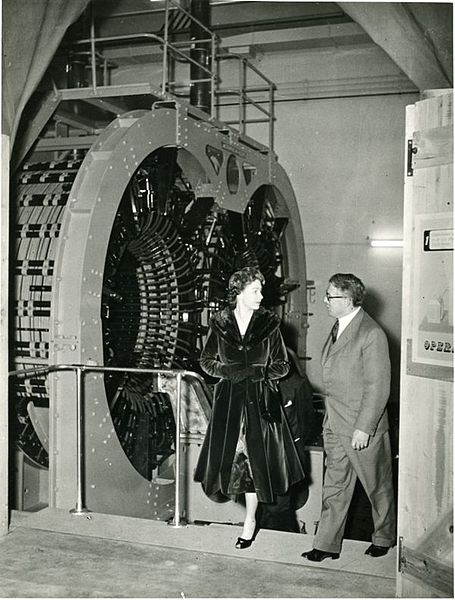
\includegraphics[width = 0.75\linewidth]{./1_Introduction/queen_at_zeta.jpg}
    \label{fig:Queen_at_ZETA}
    \caption[Queen Elizabeth II at the ZETA experiment]{Queen Elizabeth II of Canada visting ZETA during it's construction in 1957. Photograph by UKAEA}
\end{figure}%

The story of the RFP starts with the Zero Energy Thermonuclear Assembly (ZETA). Initially built as an extension of the now abandoned toroidal pinch confinement concept, ZETA was one of the leading fusion experiment of its time. Scientists at ZETA to discover the spontaneous reversal of the magnetic field associated with the most stable (quiescent) period of ZETA's plasmas \cite{Butt1966,Robinson1969}. This phenomenon was explained by J. Taylor in 1974 as a naturally result from the relaxation of the magnetic topology towards lower energy state \cite{Taylor1974}. These were the foundational documents of the RFP.

\begin{align}\label{eqn:helicity}
	K \equiv \int_{V} \vec{A} \cdot \vec{B} d\tau
\end{align}

Specifically, Taylor posited that in a toroidal plasma of finite resistivity constrained by a perfectly conducting shell, the magnetic helicity $K$ is conserved (eqn. \ref{eqn:helicity}). With this constraint, the plasma relaxes toward a state of minimum magnetic energy characterized by eqn. \ref{eqn:min_energy_condition}, where $\mu \varpropto K/ \Psi ^2$, is a constant unrelated to permeability . 

\begin{align}\label{eqn:min_energy_condition}
    \nabla \times \vec{B} = \mu \vec{B}
\end{align}

In cylindrical approximation, the solution to equation \ref{eqn:min_energy_condition} are Bessel functions (eqn. \ref{eqn:rfp_solution}) where $B_Z$ reverses in the edge if the plasma current is high compared to toroidal flux \cite{Taylor74}.

\begin{align}\label{eqn:rfp_solution}
B_z &= B_0J_0(\mu r)\\
B_\theta &= B_0 J_1(\mu r)\\
B_r & = 0
\end{align}

The magnetic topology of atypical RFP is shown in figure \ref{fig:RFP_geometry}. The relatively low $B_t$ means the RFP have several advantages over the Tokamak. In the tokamaks, powerful toroidal field coils (TF coils) are used to generate toroidal flux and keep the safety factor q above 1 in order to stabilize the plasma. This leads to limits on the toroidal plasma current depending on the the available coil generated toroidal flux. This in turns is limited by engineering constrains in terms of magnetic coil construction. The reversed field pinch avoids these constrains, and
consequently can be constructed with much simpler and cheaper TF coil arrangements, as well as being more easily reach very high current levels to take advantage of large Ohmic heating, possibly to ignition levels.

\begin{figure}[!htb]
	\centering
	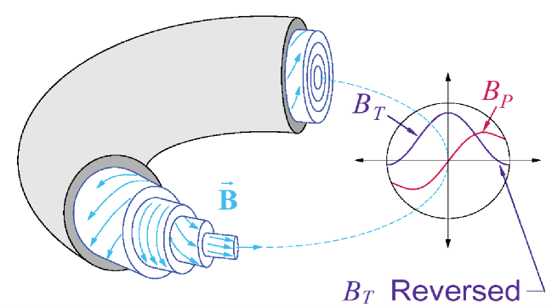
\includegraphics[width = 1.\linewidth]{./1_Introduction/RFP_mag_geometry.png}
	\caption[RFP magnetic topology]{Illustration of the RFP topology. The most distinct features of the RFP is the similar magnitudes of $B_t$ vs. $B_p$, as well as the fact that $B_p$ reverses direction near the edge.}
	\label{fig:RFP_geometry}
\end{figure}%

However, the magnetic topology also poses challenges to the RFP's confinement characteristics. Taylor noted that the relaxation of the magnetic field is made possible by the finite resistivity, but did not speculate on the 'method' of
relaxation. Experiments have shown that the relaxation occurs via resistive tearing mode instabilities which poses a challenge to RFP confinement characteristics.

\begin{figure}
	\centering
    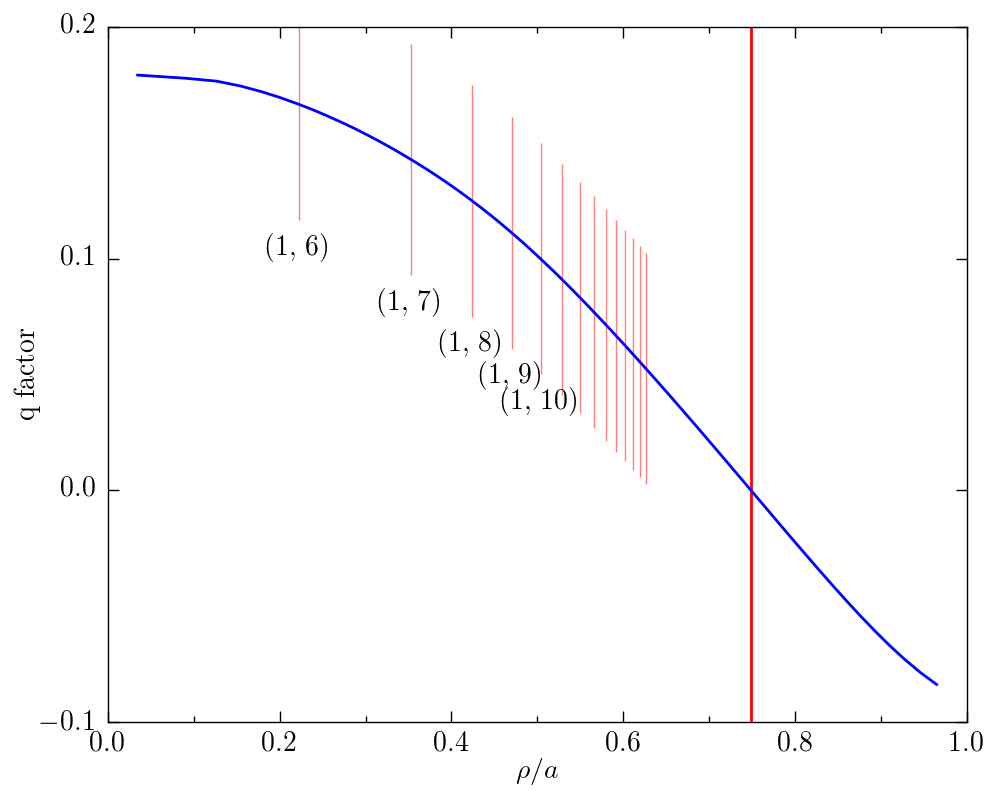
\includegraphics[width = 1.\linewidth]{./1_Introduction/PPCD_q_profile.png}
    \caption[Example RPF q profile]{q profile typical of the plasmas studied in this work. Note the closely space resonant surfaces near the reversal surface. These plasmas have a deeper reversal than standard RFP operation due to the confinement improvement techniques explored in the next chapter.}
    \label{fig:q_profile}
\end{figure}

The finite resistivity of the plasma allows for the reconnection of the magnetic field lines and the formation of magnetic islands through tearing mode instabilities. Tearing modes are unstable at magnetic resonant surfaces where the safety factor $q \equiv \frac{rB_T}{R_0B_p}$ is a rational number, ie $q = \frac{m}{n}$ where m and n are integers. The location of these unstable regions
form 'resonant' surfaces that are typically labeled by their m and n numbers. The RFP have q significantly lower than 1 everywhere, and further decreases monotonously towards the edge where it will cross 0. An example q profile is show in figure \ref{fig:q_profile}. This leads to the existence of a large number of resonant surfaces, especially close to the reversal surface. 

These closely spaced resonant surfaces and the tearing mode instabilities that they 'host' creates regions of overlapping magnetic islands that turns the magnetic field stochastic, greatly reducing the confinement characteristics. The primary drive of the tearing mode instabilities are the current density gradient\cite{Schnack1987,Ho1991}. Specifically $\nabla\lambda$ where,
\begin{align}
    \lambda &= \frac{J_{\parallel}}{B}\\
    &= \frac{\vec{J}\cdot\vec{B}}{B^2}\nonumber
\end{align}
where $J$ is current, $B$ is magnetic field, and all quantities are flux surface averages. In standard RFP operation, the $\lambda$ profile tends to peak in the core of the plasma as the result of current drive, providing free energy to core resonant tearing modes. As the current peaks, the core tearing modes grow and non-linearly couples to each other, until they are sufficiently large to trigger a violent relaxation event called a sawtooth crash. This redistributes the current profile such that toroidal current in the core decreases while the poloidal current in the edge increases\cite{Terry2004}. This effectively flattens the $\lambda$ profile and decreases the drive of the tearing instabilities. But the process repeats as the current profile peaks again in a cycle that is referred to as the sawtooth cycle. Though ion heating is observed with the sawtooth crashes\cite{Bodin1980}, they greatly decreases confinement and is undesirable for fusion development.

\section{Improving confinement with inductive current profile control}

One successful way of improving confinement on the RFP, therefore, is through the control of $J_{\parallel}$ profile. This is done inductively on MST through a process called Pulsed Parallel Current Drive (PPCD). PPCD can be thought of as 'helping' the plasma to drive parallel current in the edge region, and thereby flattening the $\lambda$ profile\cite{Sarff1995}. In particular, a series of 4 high voltage capacitor banks discharges are used to apply voltage to the toroidal field circuit. This result in a series of 4 poloidal field pulses, which raises $E_{\parallel}$ in the edge. Thus, PPCD is a transient current drive and profiles of the RFP continually evolve during this period. 

With successful applications of PPCD, sawtooth cycles are interrupted which allows a new class of dynamo events called m = 0 bursts to come to the forefront. Details regarding these m=0 bursts are discussed in chapter \ref{ch:m0}. In the meantime it suffice to say that the frequency of these m=0 bursts can be significantly reduced by reversing the applied toroidal electric field in the edge of the plasma\cite{Chapman2001}.

\begin{figure}
    \centering
    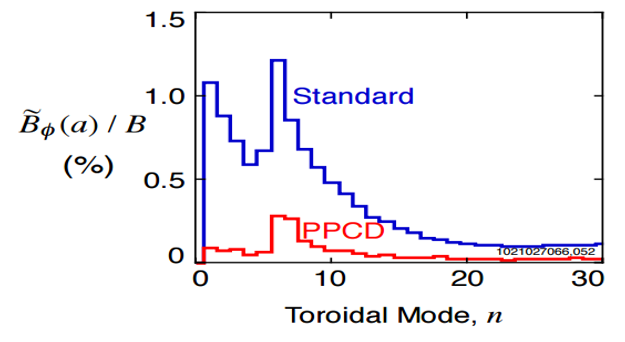
\includegraphics{./1_Introduction/ppcd_fluc.png}
    \caption[Typical tearing mode amplitude in PPCD]{Typical tearing mode amplitude in PPCD.}
    \label{fig:ppcd_fluc}
    %TODO: consider remaking this plot for my particular plasmas if time allows
\end{figure}

PPCD reduces the tearing mode fluctuation levels significantly as shown in figure \ref{fig:ppcd_fluc}, and during the period of improved confinement, $T_e$ is known to increase dramatically as compared to standard MST plasma, while $T_i$ is observed to be relatively flat, resulting in temperature differences as high as $T_e \approx 2T_i$ in the core of the plasma. At the same time, recent observations shows that drift wave turbulence, likely associated Trapped Electron Mode, continues to be present in PPCD plasma in the edge. 

Though the electron transport properties in PPCD have been studied as part of several thesis previous, the ion transport, particularly the ion thermal transport has not been studied in the same detail. This has hampered past efforts at studying anomalous heating that results from sawtooth events. Characterizing ion thermal transport dynamics in the RFP would help establish a baseline for investigation of more complex heating phenomenons, in addition to the inherent value of understanding the ion thermal transport itself, and the identification of key energy loss mechanisms.

\section{What this thesis is about: 1-D classical transport modeling}

This thesis project aims to characterize the ion thermal transport in MST during the improved confinement periods achieved through PPCD. It approaches this question by the construction of a 1-D model of thermal transport that makes predictions on ion temperature evolution from an initial condition and diagnostic measurements of plasma parameters, with exception of $T_i$ itself. The model prediction are them assessed by comparing with measurements. The model considers classical collisional mechanisms, with addition considerations for charge exchange and flow, and unlike some similar assessments previously performed, it is not an equilibrium power balance calculation (\textit{i.e.} $\partialt x \approx 0$ for relevant parameters). Instead, at it's core, it is a foreword model that have as it's core, a numerical integration of the following equation in time,
\begin{align}
    \partialt E_\text{thermal} = P_\text{e-i} + P_\text{cond} + P_\text{CX} + P_\text{flow} + P_\textit{ad hoc}
\end{align}
where the different $P$ terms denotes thermal power terms acting upon majority ion fluid, and are functions of time and $\rho_v$, the radial coordinate. This equation is revisited in more detail in section \ref{sec:transport_summary}, after the details of the terms are discussed. 

The thesis starts in chapter 2 by discussing the various physics mechanisms included in the model as well as the consideration for those that are not. Chapter 3 gets into the details of the hardware and diagnostic used to calculate the model terms, as well as considerations for the implementation and coding strategies used in the model. Chapter 4 details discoveries made working with the model analysis, including about neutrals and flow in the plasma, then discusses modeling results and comparisons to measurements, as well as the need for an \adhoc term in the edge. Chapter 5 discusses the adjacent topic of impurity heating observations during m = 0 bursts, a reconnection phenomenon that sometimes occurs during PPCD periods, following by chapter 6, a short summary of the results and directions for future work.

\begin{figure}
    \centering
    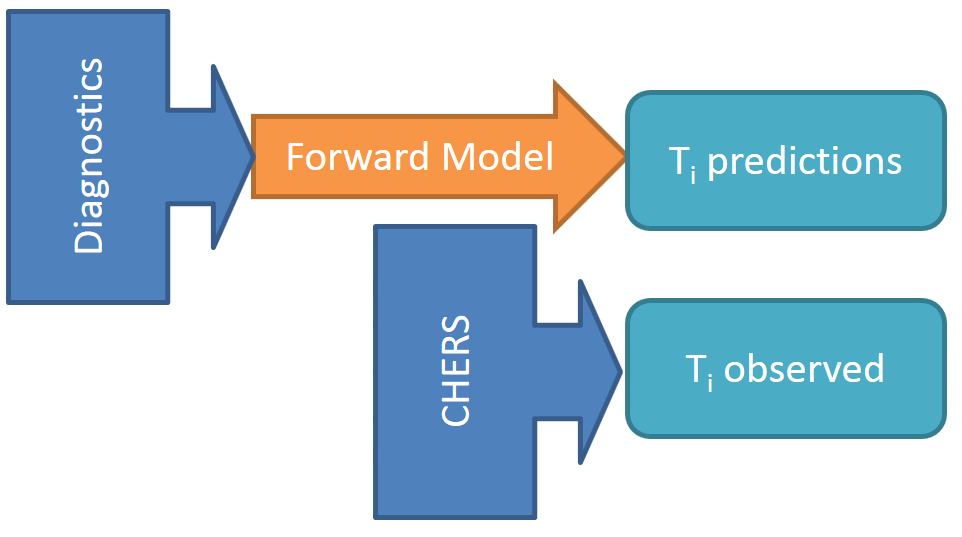
\includegraphics[width=0.75\linewidth]{./1_Introduction/exp_structure_diagram.png}
    \caption[Block diagram of experiment]{Block diagram of experiment.}
    \label{fig:ppcd_fluc}
    %TODO: consider remaking this plot for my particular plasmas if time allows
\end{figure}

\printbibliography


\end{refsection}
\begin{refsection}


\chapter{Modeling ion transport in the RFP}\label{ch:physics}

% I think you should mention that prior work on understanding on ion heating and heat transport has concentrated on understanding the mechanisms of rapid magnetic reconnection leading to rapid anomalous ion heating while also leading to rapid transport of electron heat. Cite:    % * Chapman PPCF 52, 124048 (2010)
% * Gangadhara S, Craig D, Ennis D A, Den Hartog D J, Fiksel G
%     and Prager S C 2007 Phys. Rev. Lett. 98 075001
% * Gangadhara S, Craig D, Ennis D A, Den Hartog D J, Fiksel G 
%     and Prager S C 2008 Phys. Plasmas 15 056121
% What's new here is that you are considering the ion heat transport under quiescent conditions in the best performing MST plasmas and that even in the absence of strong, rapid reconnection events there are heating mechanisms still present, particularly in the edge of the plasma. Then cite   

A full understanding of ion transport is a broad topic and difficult to tackle. Past efforts to understand transport in MST has concentrated on the sawtooth crash and it's effects on transport. The magnetic reconnection of the sawtooth events leads to rapid and anomalous ion heating as well as rapid heat loss from electrons\cite{Chapman2010}
%WORK IN PROGRESS

To make the problem more tractable, it was decided to focused on the improved confinement regime achieved through PPCD. Unlike improved confinement through Quasi-Helical State (QSH), PPCD plasmas are highly axisymmetric and have reduced stochasticity, making it ideal for a simplified 1-D model. Previous work have established preliminary 0-D and 0.5-D power balance for the ions\cite{??} which are limited in usefulness as it cannot distinguish the likely difference that exists between the core and the edge/gradient region. A 1-D model is the logical next step in investigation ion transport and anomalous heating. This chapter aims to examine the ion thermal transport physics being included in the model and some of those that are not. Starting with the relatively simple to calculate, I will briefly review thermal equlibration between electron and ions, as well as classical collisional thermal diffusion. Then I will discuss the effects of neutral particles and the particle flow on transport. The proper treatment of neutrals are important due to a combination of the fact that the other active terms are small in PPCD. Further, charge exchange neutrals are not confined by magnetic fields, giving then outside influences on a per reaction basis, as well as unintuitive behaviors. This is followed by a discussion of neoclassical and stochastic effects on heating transport and why they are not modeled by the code. At the same time, I aim to separate in the reader's mind, their effects on particle transport vs on thermal transport, and how they are ultimately treated in the final comparison with data. 

Note that this chapter has a large number of viable being introduced, and it is not always practical to note their meaning with every equation. Please refer to appendix \ref{app:term} where one would find notes on notation and terminology. 

\section{Modeled ion transport mechanisms}
This model is an attempt to catalog and characterize heating terms that are known to be active and isolate and describe the extent of what we do not know (ie. anomalous heating), and from there, investigate mechanisms that would produce the anomalous heating. In this section, I explore the known heat transport mechanisms being modeled and their general physics basis and characteristics. Some of these mechanisms also couples with particle density change, which may result in the phenomenon where the power is positive (ie, ion thermal energy increasing) but the ion temperature is decreasing. This is discussed in more detail in appendix \ref{app:term}

\subsection{Ion electron equilibration}

In a plasma where the temperature is different between two species, Coulomb collisions causes a transfer of thermal energy from the hotter to the colder. This is thermal equlibration. In PPCD plasmas, the electron confinement is significantly improved compared to standard RFP, and $T_e$ rises significantly both compared to the pre-PPCD period, to levels significantly above $T_i$. Thus, equlibration is a heating term for the ions. This is a reflection of the fact that MST is (primarily) Ohmic heated device, which is nearly entirely an electron heating mechanism. Particularly in PPCD plasmas where anomalous heating mechanisms available to ions are reduced, the thermal equalization becomes important. The equalibration power can be calculated as:
\begin{align}
    P_{ei} &= \frac{3}{2}n_i\nu^{i/e}(T_e - T_i)\\
\end{align}
where $\nu^{i/e}$ is the thermal equalibration frequency, defined:
\begin{align}
    \nu^{i/e} = 5.69\times10^{-27}\frac{(m_e m_i)^{1/2}(Z_e Z_i)^{2} n_e ln \Lambda}{(m_iT_e + m_eT_i)^{3/2}}
\end{align}
It is important to note that $\nu^{i/e}$ is not the Lorentz collision frequency but is related to the energy relaxation frequency. Due to the mass discrepancy between ions and electrons, energy transfer between the two is small per collision. Thus, the calculated equlibration heating from the even the lower temperature edge region is relatively small even though the collision frequency, in the normal sense, is relatively fast. This fact is behind the fact that in PPCD $T_e$ is 'allowed' to rise far above $T_i$. A typical profile is shown below:

\begin{figure}[!htb]
	\centering
	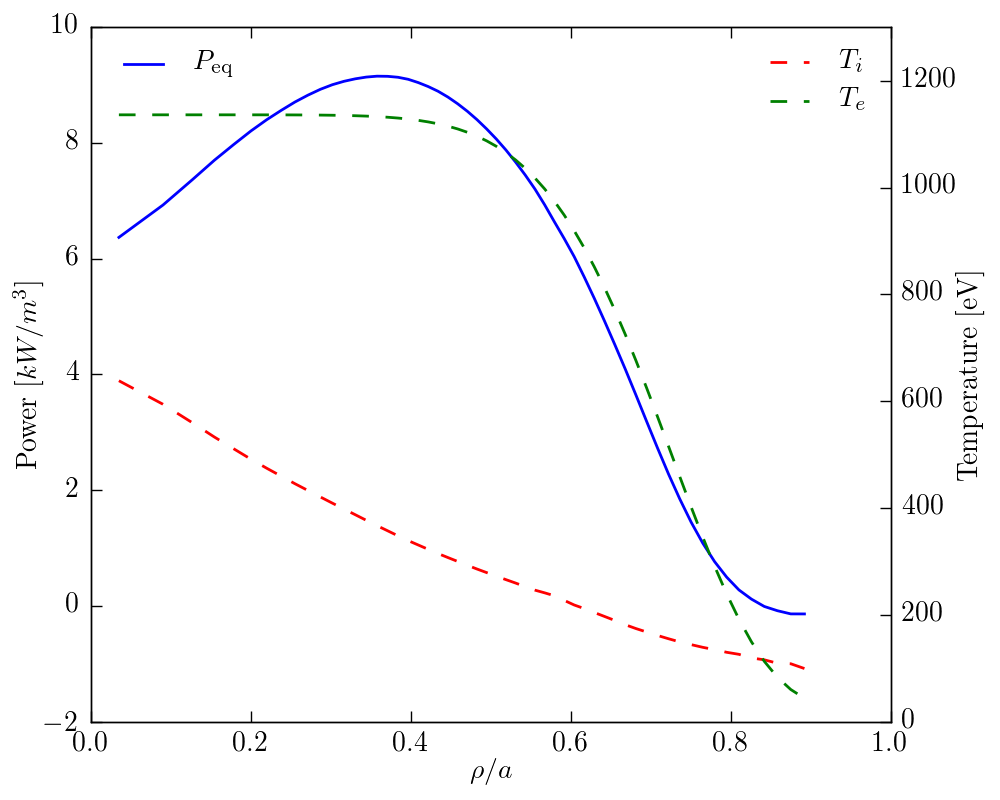
\includegraphics[width = 0.75\linewidth]{./transport_modeling/p_eq.png}
    \label{fig:P_eq}
    \caption[Example equlibration power profile.]{An example of equlibration profile in PPCD plasma conditions. The plot also show the $T_e$ and $T_i$ that forms the basis of this calculation.}
\end{figure}%

\begin{figure}[!htb]
	\centering
	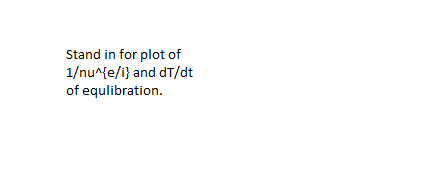
\includegraphics[width = 0.75\linewidth]{./transport_modeling/tau_eq.png}
    \label{fig:P_eq}
    \caption[Electron ion thermal equlibration time]{An example of equlibration profile in PPCD plasma conditions. The plot also show the $T_e$ and $T_i$ that forms the basis of this calculation.}
\end{figure}%

This heating term would increase slightly as the PPCD period progress, due to the increase in $T_e$ and the relative constancy of $T_i$. However, the increase in heating is smaller than what might be expected at first sight as the increase in temperature decreases the collisionality. This may indicate that Ohmic heating is not efficient for ion heating. 

\subsection{Classical thermal conduction}\label{sec:thermal_cond}

Classical thermal conduction refers to the heat diffusion due to Coulomb collisions. Note that this is not the same as the particle transport and the thermal energy associated with that movement. In an cartoonish approximation, thermal diffusion is caused by a hotter ion colliding with a colder ion on an adjacent field line during their gyro-orbits. Energy, or possibly position is exchanged, however, the center-of-mass velocity is conserved and thus no net particle flow results. The thermal conduction is thus dependent on the temperature gradient and can be calculated as\cite{Braginskii1965}:
\begin{align}
    P_{cond} &= \nabla\cdot\vec{q}_{\text{cond}} \\
    &= \frac{1}{\rho}\frac{\partial}{\partial\rho}(\rho\kappa_{\perp}\nabla T_{i})\\
    \kappa_{\perp} &= \frac{2n_ikT_i\nu_i}{m_i\omega_{ci}^2}
\end{align}

In comparison with the other terms in play, the thermal conduction term is small and can largely be ignored. It is, however, simple to calculate and still included in the model. A typical $P_{\text{cond}}$ profile is presented below. As one would expect, the term is most active in the edge where the gradient is steep and collisionality is high.

\begin{figure}[!htb]
	\centering
	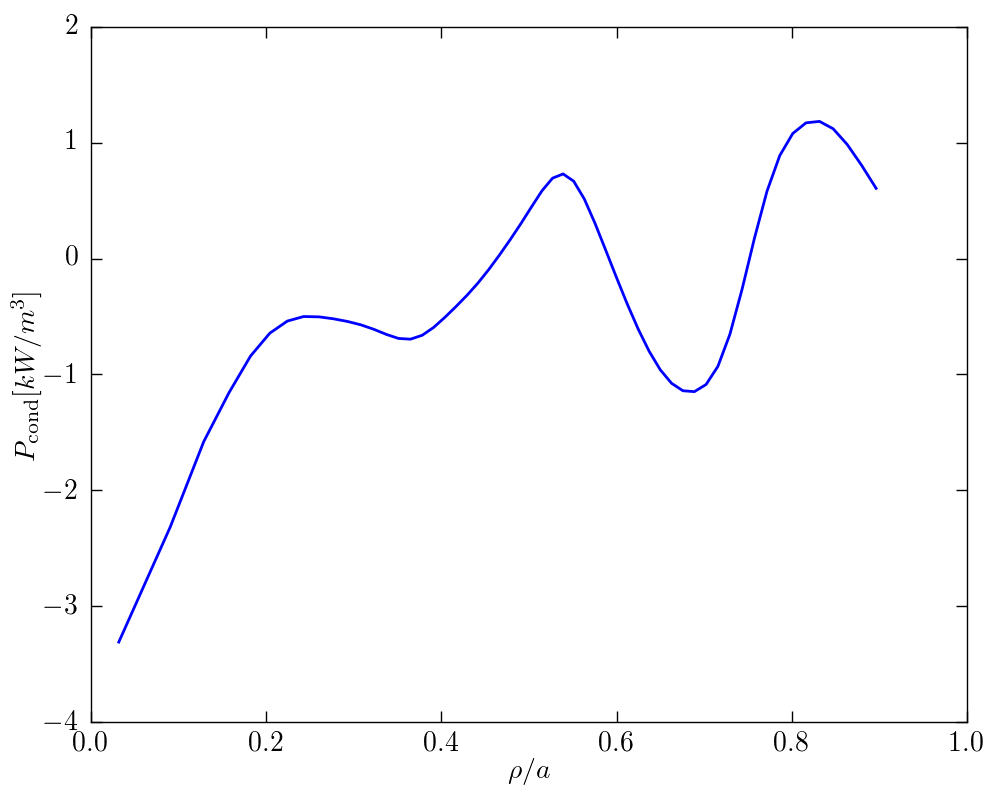
\includegraphics[width = 0.75\linewidth]{./transport_modeling/p_cond.png}
    \label{fig:P_eq}
    \caption[Thermal conduction profile]{An example of thermal conduction profile. Note the axis, this term is significantly below the equlibration term presented above, and most of the terms that I'll present later.}
    \label{fig:p_cond}
\end{figure}%

\subsection{Charge exchange and neutral transport}\label{sec:neutral_physics}

MST's thermal transport is significantly affected by the neutral population through charge exchange. Charge exchange is the process where a neutral particle, typically atomic deuterium for MST, 'gives' it's electron to an ion due to a collision. This causes the hot ion to become neutral and thus un-confined. Although the neutral fraction of the plasma is very low, charge exchange can have an out-sized effect due to the neutral essential 'by-passing' the entire magnetic confinement concept. This is especially significant in improved confinement (PPCD) plasmas where other mechanisms are reduced. The charge exchange loss can be calculated as:
\begin{align}
    P_{CX} = n_0 n_i <\sigma v>_\text{CX} (T_i - T_0)
\end{align}
where $T_i$ is the ion temperature, $T_{0}$ is the neutral temperature.

In previous estimates, the neutral fluid is assumed to be cold, therefore, exchange collisions tends to equlibrate ions with this "cold" neutral fluid. However,the mean free path of a "cold" neutral is
very short (<1cm), but edge neutrals may undergo subsequent charge exchange collisions resulting in higher temperature neutrals that can penetrate into the plasma. Consequently, neutrals in the core are mostly generated near the mid-radius and have a temperature comparable to mid-radius ions. At the same time, a charge exchange neutral created from thermal neutral in the core, if traveling through core-like conditions, has a mean free path
shorter than the minor radius, implying a fraction of such neutrals would undergo secondary ionization or charge exchange reactions. 

\begin{figure}[!htb]
	\centering
	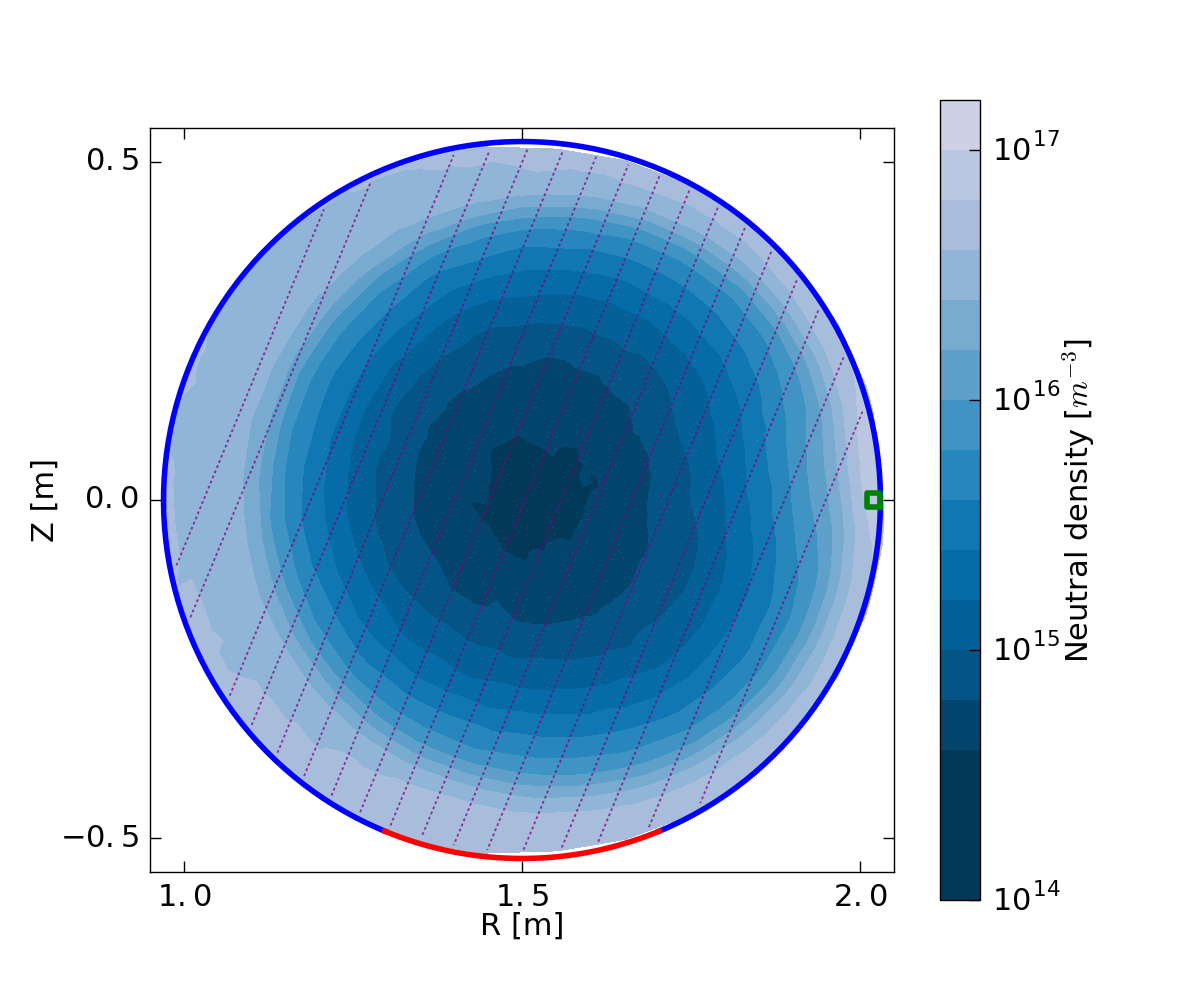
\includegraphics[width = 0.75\linewidth]{./transport_modeling/neutral_n.png}
    \label{fig:n_n_0}
    \caption[Typical neutral density profile]{A typical neutral density, as you can see, there is nearly 3 orders of magnitude drop between edge and core densities. This makes the determination of the core density difficult without modeling efforts. The analysis that produced this density profile are explained in more detail in section \ref{sec:neutral_dynamics}}
\end{figure}%

As far as terminology and conceptualization is concerned, the charge exchange 'transport' is presented as two terms in the modeling. The first is the charge exchange term itself $P_{CX}$, in which when an charge exchange reaction occurs, the difference in energy is considered lost from the ion fluid immediately. This lost energy is not entirely lost, but instead should be thought of as part of the neutral fluid's thermal energy. This thermal energy both reduces the $P_{CX}$ by reducing the temperature difference between the ion and the neutral fluid, but also may undergo subsequent electron impact ionization, by which the associate thermal energy will come back to the ion fluid. This is marked as a separate term noted as $P_{e-imp}$. It is important to note that while the electron impact brings the thermal energy 'back' to the ion fluid, it does not (typically) cause heating as the process is also a particle source term that (typically) is adding a cooler ion to the fluid. The consequences of mechanisms that contributes both particle and heat are discussed more directly in Appendix \ref{app_sec:power_terms}.

From a diagnostic point of view, the neutral density is not a straight forward quantity to measure. The neutral density drops precipitously towards the core of the plasma where the temperature is high. Measurements of neutral emissions, in MST's case the deuterium Balmer-alpha line emission, only reflects the edge neutral density as that's where the emission is coming from. The emission from the core is so low such that it is buried in the noise and fluctuations of the edge emission. Therefore, physics-based equilibrium modeling is needed to construct self-consistent core neutral profiles that produce the observed $D_{\alpha}$ emissions. Temperature would be even more difficult to measure as it's not accessible with typical spectroscopic methods. Recently on the HIT-SI3 experiment, researchers have been able to use a two-photon Laser Induced Florescence diagnostic to directly measure the density of temperature of deuterium neutrals\cite{Elliott2016}. However, such a diagnostic is not available for MST and would likely be unable to measure the low neutral density expected in MST's core. 

Instead, Monte Carlo modeling are used to solve the issues detailed above. Monte Carlo modeling uses representative particle which are drawn from a distribution. Their location and velocity is tracked, and relevant physical interactions and reaction are simulated with appropriate physics based probability distributions. The 'fate' of any given particle is fairly random is not particularly illustrative, but the simulation uses a large quantity of test particles for the simulation such that an adequate number and distribution is reached in the resulting quantities of interest. For this work, the particular quantity of interest is not only the neutral density and temperature, but also the two power terms described above( $P_{\text{CX}}$ and $P_{\text{e-imp}}$) which are tallied through the simulation directly. The simulation code used to achieved this is DEGAS2 developed at PPPL\cite{Stotler}, and the details of it's implementation as part of the model are detailed in section \ref{sec:DEGAS2}. The result from the neutral simulation regarding the charge exchange loss and electron impact ionization is complex and will be presented more fully in section \ref{sec:neutral_results} after the implementation of DEGAS2 have been described. 

\subsection{Particle flow, compression, and decompression}\label{sec:flow_effects}

When an ion moves, it carries its thermal energy with it. In this section I will speak generally regarding flow, but in the modeling work only the radial flow are considered as the symmetry assumptions implies no meaningful effects from toroidal and poloidal flow. The particle continuity equation can be written as:
\begin{align}
    \partialt n + S_{tot} = -\nabla\cdot(n\vec{V})
\end{align}
where $S_{tot}$ is the total source term. Extending the continuity equation to the thermal energy carried by the particles, and ignore the source term by focusing on the effect of the particle flow, we get:
\begin{align}\label{eqn:thermal_continuity}
    \partialt nT = -\nabla\cdot(nT\vec{V})
\end{align}
In an compressible fluid, however, there is the potential of compression work by external sources, so the equation becomes:
\begin{align}
    \frac{3}{2}\partialt nT &= -\frac{3}{2}\nabla\cdot(nT\vec{V}) - nT\nabla\cdot\vec{V}\\
    &= P_{\text{flow}}\nonumber
\end{align}
where the right side term is the \emph{compressional work} term, and the left side term is the \emph{flow conservation} term. For convenience of reference in the rest of this work, we define $P_{\text{comp work}} \equiv - nT\nabla\cdot\vec{V} $, and $P_{\text{flow cons}} \equiv -\frac{3}{2}\nabla\cdot(nT\vec{V})$.


\subsubsection{A discussion on which velocity is proper in calculation thermodynamic compressional work}

The compressional work term needs a more detailed examination from the fact that not all net decompression would invoke the work term. This makes it important the 'correct' velocity is used to calculate the work term. To begin, consider the difference between adiabatic expansion and Joules free expansion. In adiabatic expansion, an gas in an fully insulated chamber expanded against a 'piston' and does work on it. The net power on the gas is thus $P_{\text{work}} = - PdV$ where $P$ is pressure and $V$ is volume. Joule free expansion, is where there is two adjacent chambers, one of which is filled with a gas with finite temperature and pressure, and the other is in perfect vacuum. The two chambers are perfectly insulated. At a $t=0$ the wall between the two chambers are broken and gas from the first chamber is allowed to flow to the second until the pressure equlibrates. In this process, the expansion does no work, and not net energy is lost, it merely moved to be spread over a larger space. 

To examine the implications on plasma, we can start with a thought experiment. Imagine a  slab plasma adjacent to a perfect vacuum confined by a static magnetic field at equilibrium. The plasma have finite temperature with no transport mechanisms active except for what is about to be specified. The plasma is not perfectly confined, and a small flux of particles are being lost to the vacuum. In this situation, the only energy lost is that carried by the particle flux, without a work term. As a result, the temperature (energy per particle) of this plasma would not change. If the $- nT\nabla\cdot\vec{V}$ work term was to be applied in this situation, then the temperature of the remaining plasma would cool, which would conflict with the understanding of microscopic mechanics of plasma. This situation would be analogous to the Joules free expansion mentioned above, with the 'wall' in the joules free expansion case replaced with an imperfectly confining magnetic field. By a similar analogy, plasma compression via the movement of a perfectly confining magnetic flux surface can be compared to a compressing piston. It's useful to note that there is no free compression. If compression occurs, then \emph{something} has done work, and it's a matter of finding what. This is also why free expansion is considered an irreversible process, as there is no equivalent reversing process.

In real PPCD plasmas, however, these two mechanisms are not so easily separated. During the early phase of PPCD, the reversal surface is observed to move inwards, as does the $n_e$ gradient region. As will be discussed in section \ref{sec:eb_pinch}, there is an inward pinch likely related to an $\vec{E}\times\vec{B}$ drift. However, in the outer half of the plasma the net particle flow is outwards across flux surfaces due to particle transport mechanisms outside of the consideration of this thesis. This, in the thermodynamic analogy, would be akin to a leaky piston moving inwards, but the net particle velocity being outwards. The velocity use to calculate $P_{\text{flow cons}}$ should be the net velocity, as the the ions will carry their energy with them whatever the 'reason' of their movement. However, the velocity used in the work term should be the velocity associated with the mechanism by which the work is done. In this case, the \ecb drift and the movement of the flux surface associated. The implementation and consequences of this, as well as the determination of the \ecb flux and it's association with compression is discussed in much more detail in section \ref{sec:eb_pinch}.

\section{Unmodeled terms and mechanisms}

\subsection{Neoclassical effects}
\begin{figure}[!htb]
	\centering
	\includegraphics[width = 0.75\linewidth]{./transport_modeling/banana_width.png}
    \caption[Banana width and ion trapped fraction in PPCD]{Banana width and ion trapped fraction in high current PPCD. This also qualitatively applies to nearly all RFP plasmas. The primary 'cause' of this is the low $B_t$ that RFPs use to confine the plasma.}
    \label{fig:banana_width}
\end{figure}%
Neoclassical effects are, in approximation, those that arises due to the toriodal nature of the magnetic confinement devices. In short, due to the nature of Ampere's law, $B_t$ on the inboard side is higher than the low field side, and drops as $~1/R$. This fact is important enough in the Tokamak world that the inboard side is typically referred to as the high field side, and the outboard side being the low field side. As a given field-line travels poloidally around the plasma volume, particles see varying $|\vec{B}|$ and effectively experiences a magnetic mirror. The portion of particle with in sufficient $B_{\parallel}$ to complete the journey around poloidally are referred to as trapped. They are reflected by the mirror effect and 'attempts' to retrace it's steps. But $\nabla B$ and curvature drifts give the poloidal path of the particle a certain width, giving it a crescent shape. This is called the banana orbit, and the width the banana width. For the Tokamak geometry, the existence of the banana orbit enhances the collisional transport experienced at low collisionality regimes since a collision may move a particle a banana width from it's previous orbit average location instead of a gyro-radius. This effect goes away as the collisionality increase as the particles are no longer able to complete banana orbits before collisions alters their path. Further, the collisional transport is typically not \emph{directly} effected by neoclassical considerations. While the banana width is larger than the gyro-radius in Tokamak geometry, that is not typically the case for RFPs including the MST. The average banana width only exceeds the gyro-radius near the core, where the trapped fraction is small. In the low collisionality Pfirsch-Schluter regime, the neoclassical diffusion coefficient is to a first approximation $D_{P-S} \approx \frac{q^2}{\epsilon^{3/2}}D_{\text{classical}}$

\begin{figure}[!htb]
	\centering
	\includegraphics[width = 0.75\linewidth]{./transport_modeling/neo_class_ratio.png}
    \caption[$\frac{q^2}{\epsilon^{3/2}}$ in PPCD]{A plot of $\frac{q^2}{\epsilon^{3/2}}$. It is under 0.2 for the entire plasma, thus the neoclassical transport is below the classical diffusive transport for entire volume, and could be safely ignored.}
\end{figure}%

The trapped particle populating will also affect the plasma stability, turbulence, and thus effect the transport properties indirectly. For example, the neoclassical correction to the Spitzer resistivity is important for the electron thermal transport, and trapped-electron mode turbulence is also known and measured for PPCD plasmas. These are not with in the scope of this thesis. However, they are not so much ignored but Incorporated indirectly. The electron temperature is measured and used as an input to the model, so it effectively accounts all electron physics at or slower than the cadence of measurement. The effect of any induced particle transport is indirectly incorporated through the particle continuity equation, and the determination of net particle flux, discussed in section \ref{sec:eb_pinch}

\subsection{Stochastic effects}\label{sec:stochastic_effects}
No discussion of transport in the RFP is complete without a discussion of the effects of stochasticity. However, the full effects of stochasticity is not known to an analytically extent. In their well known paper, Rechester and Rosenbluth\cite{Rechester1978} detailed a way to compute thermal diffusion due to stochasticity. However, previous work on electron thermal transport in MST finds that it poorly describes the observations made \cite{Reusch2011}. To more accurately understand the effect of stochasticity, thesis-es worth of complex simulation modeling work needs to be done. Further, stochasticity is not static, but inextricably linked with fluctuations and turbulence. In the case of ions, stochasticity is proposed as a heating mechanism associated with sawtooth events\cite{Fiksel2009}. Being that stochasticity is both reduced in the PPCD plasma, and that it is likely associate with the anomalous heating that I aim to isolate and investigate, I take the approach of categorizing the stochastic effects on heat transport as a part of the anomalous heating. An quantification and localization of the anomalous heating is instructive in the discussion and investigation into stochastic mechanisms, and this will be discussed in more detail in section \ref{sec:anomalous_heating}.

It is important to note that similar to neoclassical effects on particle transport, the stochastic effects on \emph{particle transport} is indirectly included via the continuity equation, as the density observations are treated as an input parameter. Whereas the stochastic effects on \emph{thermal transport} is treated as anomalous.

\section{Summary of ion thermal transport in the RFP}

In this chapter I have laid out the ion thermal transport physics incorporated into the model. Starting with the simple, classical thermal equlibration between electron and ions, and the classical collisional thermal diffusion, both of which are well known and easy to calculate. The transport effects of the neutral fluid and particle flows are more complex, and as you will see, forms a significant part of the work of this thesis work. The proper treatment of the neutrals and especially the fact that they have a temperature is important to quantifying their effects, and in the result section I will demonstrate that the $P_{CX}$ can exhibit behaviors that are not intuitive, especially within the $Q = -n\chi\nabla T$ framework where one seeks to quantify transport with a calculated $\chi$ value. 

A numerical model is built to predict 1-D ion temperature profile by calculating these terms. The model implementation will be discussed in detail in the next chapter, along with the diagnostics used. However, at it's core, the model numerically integrates the following differential equation,
\begin{align}
    \partialt E_\text{thermal} = P_\text{e-i} + P_\text{cond} + P_\text{CX} + P_\text{flow} + P_\textit{ad hoc}
\end{align}
In the simplest form, the model is a numerical integration of this equation in time, arriving at temperature predictions. The various terms being integrated at calculated at each step with the appropriate diagnostic input and equilibrium reconstruction. The end goal being a comparison of the model prediction with measurement of $T_i$ provided via CHERS. Having explored the physics being modeling in this chapter, I will go into details about the implementation in the next.  


\printbibliography%[title={Section bibliography}]
\end{refsection}


\begin{refsection}
\chapter{Implementation of ion transport model for PPCD plasmas in MST}\label{ch:implementation}

 Moving on from the discussion of transport physics, this chapter describes the implementation of the model in hardware and code. 
 %% Reworded this intro sentence a bit. Please check to see that it covers what you want to say -- MDN 
 %While sizable and important, this is likely one of the least interesting chapters in this thesis. There are no results presented here. (Unnecessary -- MDN)
 %--
 % ok -X
 The first half of the chapter deals with the diagnostics relevant to this research, their capabilities, and how they are used in the modeling. Then I will discuss the modeling methods and considerations of it's implementation.
 % These last two sentences could be much more specific by indicating that the work you are doing is related to ion heat confinement which, for the plasmas densities under study, involves understanding the evolution of the ion temperature over several ms. As such, the relevant time scale is the one on which the equilbrium magnetic pressure varies. The confinement time is 10-15 msec, but since the electrons are heating up during the discharge, the equilibrium evolves during this time. Therefore, although the small-scale dynamics responsible for transport involve much faster fluctuation time scales, the evolution of the equilibrium is well-characterized on the 1 msec (or 500 mircosecond) timescale. All the dynamics faster than this timescale are considered part of the transport physics and parameterized by advection and diffusion coefficients.
 %--
 %I edited the text to address this in more detail in the relevant section. I intend this part to be a cursory signpost as to the structure, and get into the details later. -X
 At it's core, this modeling work is a compromise between making it simpler through approximations so that it could be better understood and completed in a reasonable time, but still preserving enough details and grounding in data so that it produces insightful and believable results. In someways, this chapter describes and justifies those compromises. 

%===========
%====MST====
\section{A summary of MST and it's diagnostics}\label{sec:MST}
Let's begin with the plasma experiment itself. The Madison Symmetric Torus is a reversed field pinch experiment located in Madison, WI. It was constructed in the 1980s, achieving first plasma in 1988\cite{Dexter1991}. It was designed as a proof of concept device to demonstrate the RFP fusion\cite{Najmabadi1999}, and a number of advanced diagnostics were designed and fielded on the MST as part of this role. The MST is capable of a wide range of plasma conditions and configurations, and improved confinement through current profile control was achieved and refined in the late 1990s\cite{Sarff1995, Chapman2002}. This method, referred to as Pulse Parallel Current Drive (PPCD) is a transient process that greatly reduces the tearing mode fluctuations that leads to heat transport by stochastization of the magnetic field in the standard RFP plasma. To help achieve consistent PPCD plasmas at high currents, the walls are well conditioned, no probes are inserted, and gas puff fueling is carefully timed to precede the PPCD period. These plasmas are too hot for probe measurements, but instead, a variety of noninvasive advanced diagnostics provide information about the core plasma including interferometry, Thomson scattering measurements, and visible light emission measurements. An array of magnetic pickup coils in the walls provide boundary magnetic measurements. 

\begin{figure}[!htb]
	\centering
	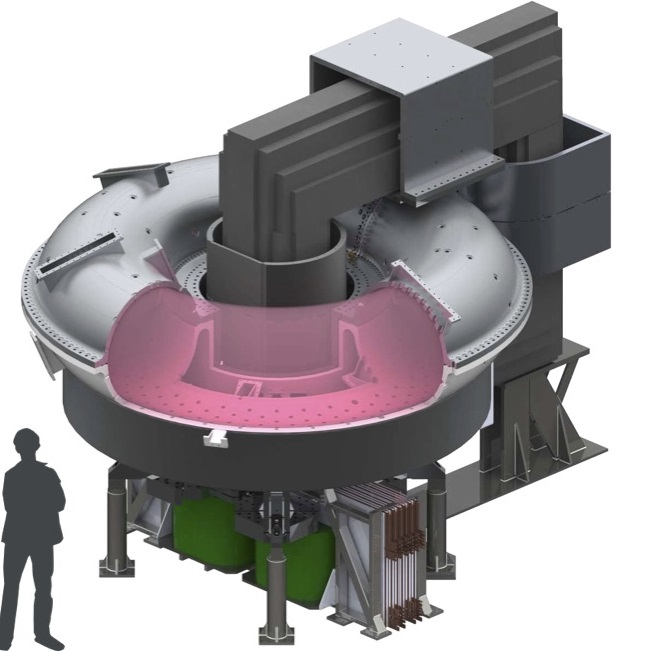
\includegraphics{./implementation/MST_model_diagram}
	\label{fig:MST_diagram}
	\caption[Diagram of MST]{Diagram of MST. Note the close fitting shell, as well as the holes on the bottom of the vessel that lead to the pumping manifold. Te pumping duct location will become relevant in section \ref{sec:neutral_source_geometry}.}
\end{figure}

\begin{table}[]
    \centering
    \begin{tabular}{||c|c|c||}
        Parameter & MST range & experiment range\\
        \hline
        Major radius ($R$)& 1.5 [m] & -same- \\
        Minor radius ($r$)& 0.52 [m] & -same- \\
        Plasma Current ($I_p$) & 50 ~ 500 [kA] & 480 -500 [kA] \\
        Magnetic Field ($B_t(0)$) & $\leq 0.6$ [T] & $~0.5$/ [T] \\
        Electron Density ($n_e$) & $0.5 - 3 \times 10^{19}$ [$m^{-3}$] & ~$0.7 \times 10^{19}$ [$m^{-3}$]\\
        Electron Temperature* ($T_e$) & $0.05 \sim 1.8$ [keV] & $0.9 \sim 1.5$ [keV] \\
        
    \end{tabular}
    \caption[MST parameters]{Basic parameters of MST. The experiment range refers to the parameters of the high current improved confinement plasmas considered as part of this work. }
    \label{tab:my_label}
\end{table}


%\begin{figure}[!htb]
%	\centering
%	\includegraphics{./implementation/MST_diags.PNG}
%	\label{fig:MST_diagnostic_diagram}
%	\caption[Diagram of diagnostic locations]{A diagram of the MST diagnostics. For PPCD, the toroidal separation of the diagnostic is typically not very important due to the good asymmetry displayed by the plasma. However, for the m=0 burst studies detailed in chapter \ref{ch:m0}, it becomes more relevant. }
%\end{figure}

Ion transport is dependent on a large number of plasma parameters even when only classical effects are considered. Hence, a range of MST's diagnostics are used. The rest of this section aims to give a summary of the principal of operation for the key diagnostics as well as the analysis techniques used to interpret %process (MDN)
the raw diagnostic data. 

%============
%===FIR===
\subsection{Far Infrared Interferometer and Polarimeter}
The Far InfraRed (FIR) interferometer-polarimeter is a laser diagnostic that employs two different physics principles to measure electron density as well as parallel magnetic field strength. While neither measurement directly informs ion transport, they are critical plasma parameters that are needed to calculate the various terms % which terms?
in the model. I will start by giving a short introduction of the two separate physics principles of the interferometer and then that of the parameter. Then I will describe the FIR hardware as available on MST, and finally, I will describe the analysis and incorporation of raw diagnostic data. 

The FIR interferometer relies on the fact that the index of refraction of the plasma is dependent upon the density of the plasma. In short, one laser beam is passed through the plasma, and then compared with a reference beam that passed through air. The relative phase lag is measured by the interferometer and information about the plasma density is extracted. 

To understand this process in more detail, we can begin with a Fourier representation of the electric field of a generic EM wave:
\begin{align}\label{eqn:fir_wave}
    \vec{E}(\vec{x}, t) &= \frac{1}{(2\pi)^4}\int\vec{E}(\vec{k},\omega)e^{i(\vec{k}\cdot\vec{x}-\omega t)}d^3\vec{k}d\omega 
\end{align}
where $\vec{k}$ is the wave vector, and $\omega$ is the angular frequency. The magnetic field component $\vec{B}(\vec{x},t)$ is similarly described.

In a plasma, an EM wave has to further satisfy the wave equation, as well as Ohm's law, which combines into the following:
\begin{align}
    (\vec{k}\vec{k} - k^2\xtensor{\textbf{1}} + \frac{\omega^2}{c^2}\xtensor{\epsilon})\cdot\vec{B} = 0
\end{align}
where $\xtensor{\epsilon} = (1+\frac{i}{\omega\epsilon_0})$ is the isotropic dielectric constant. Taking the cold plasma approximation of $\xtensor{\epsilon}$ and simplifying the result yields the Appleton-Hartree formula\cite{hutchinson_2002},
%%%Also, you use the first-order approximation lower down, so best to solve the relation to first order here.
\begin{align}
    N^2 &= 1 - \frac{X(1-X)}{1-X-\frac{1}{2}Y^2 \sin^2\theta\pm [(\frac{1}{2}Y^2\sin^2\theta)^2 + (1-X)^2Y^2\cos^2\theta]^{\frac{1}{2}}}
\end{align}
where $N$ is the index of refraction, $X = \frac{\omega_p^2}{\omega^2}$ and $Y = \frac{\Omega}{\omega}$. Considering that the cyclotron frequency $\Omega$ is small compared to the FIR laser frequency $\omega$, then $Y \rightarrow 0$. Taking the zeroth-order approximation\cite{Hutchinson_2002},
\begin{align}
N^2 \approx 1 - \frac{\omega_p^2}{\omega^2}
\end{align}
which is only dependent on $n_e$. Under these conditions, measuring the phase difference between a beam that travels through the plasma and a reference beam traveling through the air will give phase difference
\begin{align}
    \Delta\phi &= \int(k_0 - k_{\text{plasma}})dl \nonumber\\
    &= \frac{\omega}{c}\int(N - 1)dl \nonumber \\
    &= 2.814\times10^{-15}\lambda\int n_e dz 
    &\text{\ [For MST conditions]}
\end{align}
The parameter takes advantage of the 1st order approximation of $N^2$,
\begin{align}
    N^2 = 1 - X \pm XY cos \theta
\end{align}
where the addition refers to the ordinary mode and the subtraction refers to the extraordinary mode. The two modes approximately correspond with right and left handed circularized polarization. Given the differing index of refraction for the two circular polarizations, a phase difference results, leading to an effective rotation of initial polarization referred to as Faraday rotation. The rotation angle is given by,
\begin{align}
    \alpha &= \frac{\Delta \phi}{2}\nonumber\\
    &= \frac{1}{2}(N_+ - N_-)\frac{\omega}{c}z \\
    &\approx \frac{e^2 \lambda^2}{8\pi m^2_e c^3 \epsilon_0}\int n_e \vec{B}\cdot d\vec{l} \nonumber \\
    &= 2.62\times10^{-13}\lambda^2\int n_e{\vec{l}}\vec{B}\cdot d\vec{l} &\text{[For MST conditions]}
\end{align}

\begin{figure}[!htb]
	\centering
	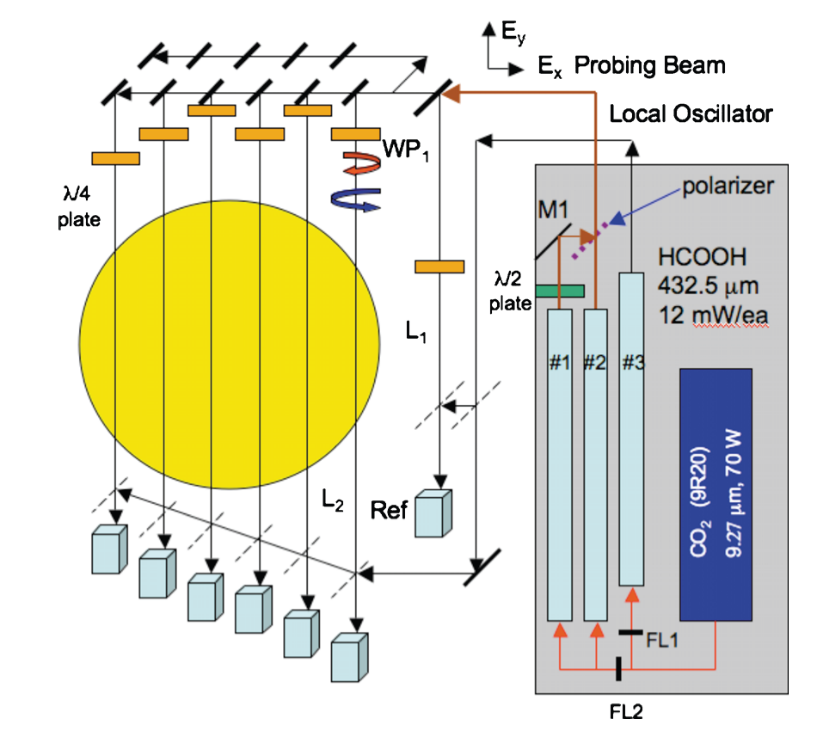
\includegraphics[width = 0.9\linewidth]{./implementation/fir_optics_diagram.PNG}
	\caption[Diagram of FIR optical paths]{Diagram of FIR system optical paths. Lasers marked \#1 and \#2 are orthogonally polarized for polarimetry measurements, and laser \#3 is used as the `local oscillator' necessary for heterodyne phase detection for the interferometry measurements. (Reproduced from E. Parke, et al.\cite{Parke2016})}
    \label{fig:fir_optics_diagram} 
\end{figure}

MST's FIR system consist of a CO$_2$ laser pumping three formic acid cavities in a heterodyne system. The three formic acid cavities are pumped using the same CO$_2$ laser in order to reduce the effects of power fluctuation on the output beam since all three beams are proportional to the pump power. The CO$_2$ pumping laser is a commercially available model with a tunable laser cavity allowing it to be tuned to the FIR pumping frequency. The formic acid laser cavities are custom built and can be tuned independently via motor mounted mirrors. The formic acid lasers convert the ~$10\mu m$ photons from the CO$_2$ laser to ~$432.5\mu m$ (~700GHz) for the probing beams. To facilitate heterodyne detection of phase, the formic acid lasers are further tuned to relative frequencies on the order of 1 MHz. The optical system splits the probing beam into 11 independent measurement chords, as well as separate reference and 'local oscillator' beams paths using thin wire mesh beam splitters. Figure \ref{fig:fir_optics_diagram} provides an illustration of the optical setup. The laser beams, after completing their designated path, are measured with recently installed planar-diode mixers at 6 Mhz. These mixers have high sensitivity and reduced noise floor allowing fluctuation measurements of up to 250 kHz for polarimetry and 600 kHz for interferometry\cite{Parke2016}. 
\begin{figure}[!htb]
	\centering
	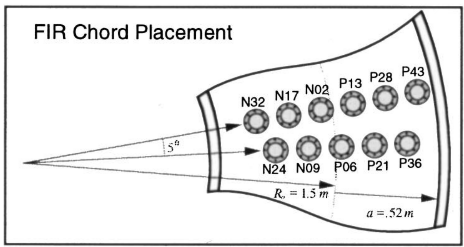
\includegraphics[width = 0.75\linewidth]{./implementation/fir_chords.PNG}

	\caption[Diagram of FIR chord offset]{Diagram of FIR system's 11 viewing chords separated into 2 sets, 5\textdegree\ apart. (Reproduced from N. Lanier, et al.\cite{Lanier2001}}	
	\label{fig:fir_chords}
\end{figure}

The 11 measurement chords are further separated into two sets, about $5\degree$ toroidally separated from each other (see figure \ref{fig:fir_chords}). This has been taken advantages of to make toroidal fluctuation measurements, but for the purpose of the PPCD plasmas investigated in this work, only their radial locations are considered. 

It is pertinent to note that the electron density profile is not determined from a simple inversion of FIR interferometry measurements, but rather incorporated as constraints with other diagnostics measurements in a Grad-Shafranov equilibrium calculation \cite{Anderson2001} as discussed in more detail in section \ref{sec:MSTfit}.

%==D_alpha==
\subsection{The $D_{\alpha}$ array}\label{sec:dalpha_array}

Neutral particle density profiles are determined by modelling the neutral particle dynamics from particle sources and sinks which are constrained by the measurement of deuterium Balmer-alpha (or $D_{\alpha}$) emissions arising from the $n=3$ to $n=2$ transition. $D_{\alpha}$ emission occurs when a deuterium atom is excited to a higher state, usually through electron impact excitation or charge exchange. The associated radiance can be calculated as,
\begin{align}
    R &= \int_C \frac{\Delta \Omega(\vec{r})}{4\pi}\gamma_{D_{alpha}}(\vec{r}) dl\\
    \gamma_{D_{alpha}} &= \frac{A_{32}}{ A_{32} + A_{31} }\left( n_0 n_e <\sigma v>_{\text{excitation}} + n_0 n_i <\sigma v>_{\text{CX}} \right)
\end{align}
% You call this quantity "the rate of photon generation," but a check of the units shows that it has units of m^-3/s. I suspect that this is the number of photons produced per volume. The usual radiometric quantity to report here is the "radiance" which has units of Watts/(m^2 Sr). This is the amount of radiant energy emitted from a surface per solid angle per time. It may make sense to write this quantity out in terms of the line-integrated emission coefficient (units of W/(m^3 Sr)) since this is what you are measuring and forward-modelling in DEGAS2.
%--
%Changed, although what DEGAS2 does is much more complicated than this integral as it uses sub-chords and calculating percent contribution of a finite volume and so on. The complications is partly why I chose originally to present the photon generation per volume per time calculation. --Xing
where $n_0$ is the neutral density, and $<\sigma v>$ are the distribution averaged reaction rates for electron impact excitation and charge exchange into the neutral deuterium $n=3$ excited state and $A_{32}$ and $A_{31}$ are the Einstein coefficients for spontaneous emission. Given $n_e$, $n_i$, and $n_0$ the neutral emission is easy to calculate, but it varies over $3$ orders of magnitude across the plasma diameter with very little emission arising from the hot core. Accurately determining the neutral density in the core requires careful calculations of the neutral dynamics which are discussed in detail in section \ref{sec:DEGAS2}.


\begin{figure}[!htb]
	\centering
	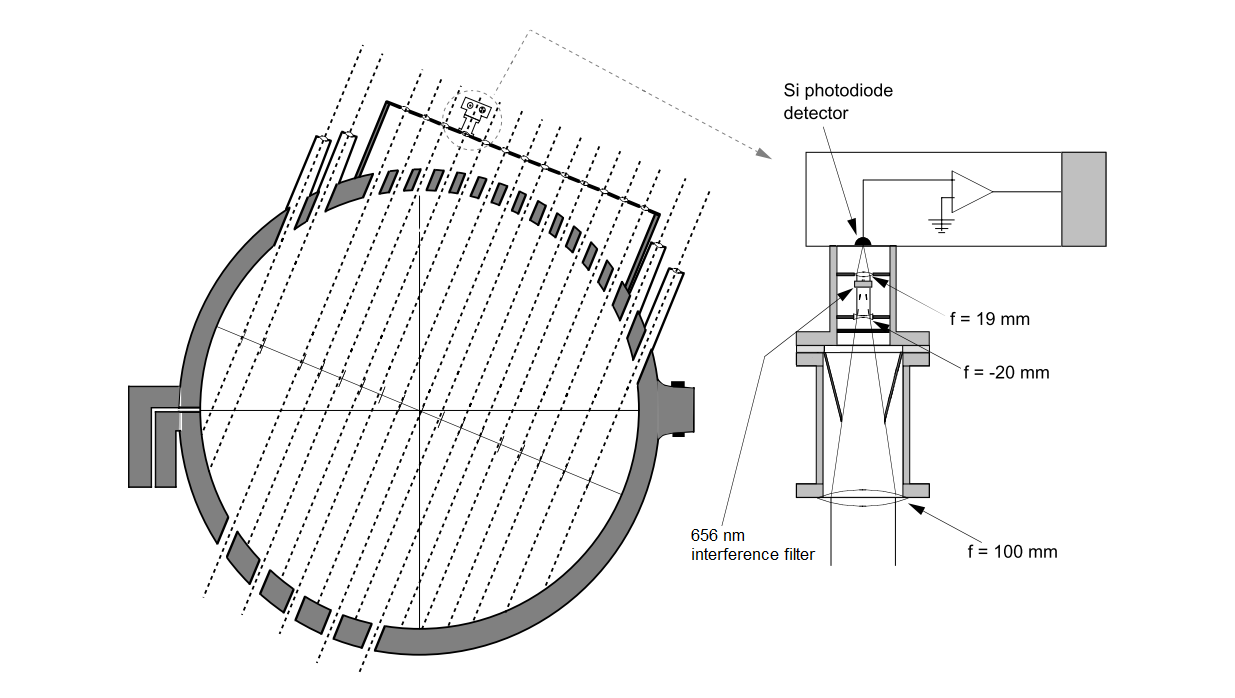
\includegraphics[width = 0.9\linewidth]{./implementation/d_alpha_detector.PNG}
	\caption[$D_{\alpha}$ detectors]{Diagram $D_{\alpha}$ detectors and available viewing chords. The detectors consist of focusing optics, a silicon photo-diode, and a trans-amplifier circuit. In some detectors there is also a pin-hole aperture used to reduce the intensity of incident light on the detector. Five of the viewing cords have matching ports on the other side, but they are not used for this work. (Reproduced with modifications from J. Anderson\cite{Anderson2001})}
	\label{fig:D_alpha_diagram}
\end{figure}

MST uses 13 silicon photo-diode detectors to observe the 656nm $D_\alpha$ line.  The detector array (referred to as the $D_{\alpha}$ array) is located at the $210 \degree$ toroidal boxport. The boxport has 17 available lines of sight, hence we are limited by the avaliable detectors. The detectors consist of filtered silicon photo diodes with a built-in current-to-voltage transimpedance amplifier. Figure \ref{fig:D_alpha_diagram} shows the physical assembly of the detectors.

\begin{figure}[!htb]
	\centering
	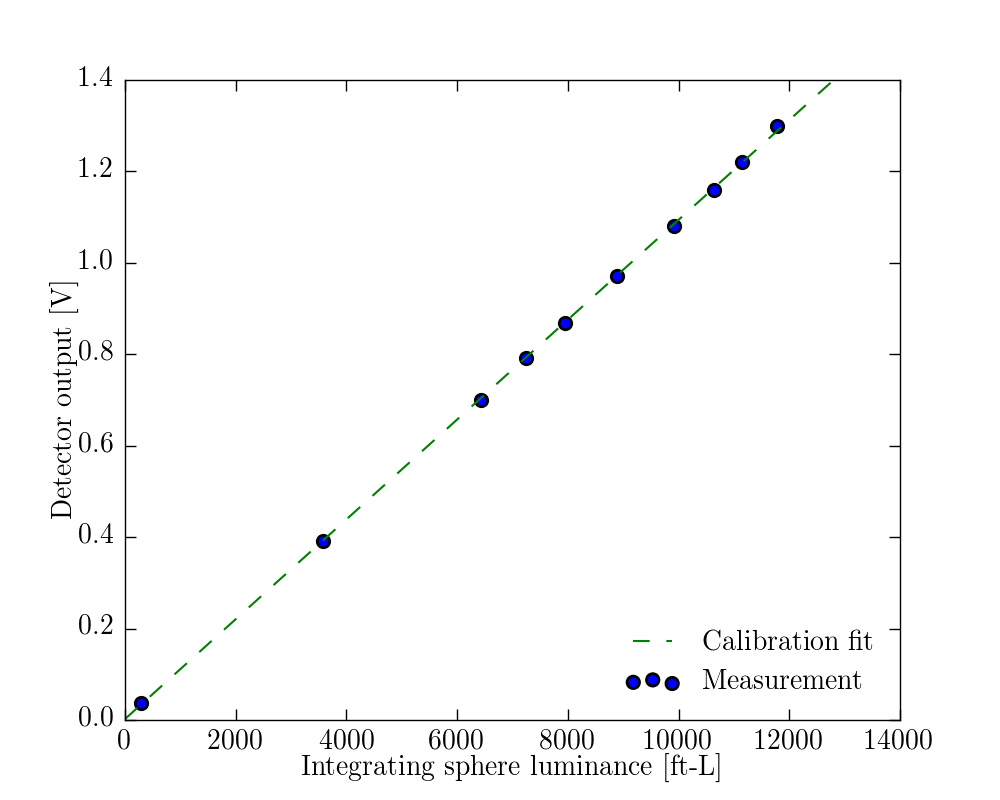
\includegraphics[width = 0.9\linewidth]{./implementation/diagnostics/l_vs_v.png}
	\caption[Example $D_{\alpha}$ calibration]{Example voltage vs luminance calibration for $D_{\alpha}$ detectors. This in particular is from detector \#32's calibration from Aug. 2015.}
	\label{fig:l_vs_v}
\end{figure}

The detectors are calibrated using a commercially available Tungsten strip-lamp with integrating sphere which has been calibrated for radiance measurements. An optical assembly identical to that on MST is used to couple light from the integrating sphere to the detector. Since the optical geometry is reproduced, the geometrical effects quantified by the {\'e}tendu $A\Delta\Omega$ are held to be constant between calibration and machine. However, the transfer function is much wider than the $H_{\alpha}$ emission line, and thus needs to be taken into account. Namely the voltage measured in calibration is
\begin{align}
    V_{\text{cal}} &= c A \Delta\Omega \int^{\infty}_{0}f(\lambda)R_\lambda(\lambda)\ d\lambda\\
    &\equiv c'R
\end{align}
where $c$ and $c'$ are calibration factors, $f(\lambda)$ is the transfer function of filter, and $R_\lambda$ is the spectral radiance of the integrating sphere. With $c'$ thus defined, it can be easily calculated from measured pairs of output voltage {\em vs} luminance slope from,
\begin{align}
    c' &= \frac{V_{\text{cal}}}{R}\\
    &= \frac{\Delta V}{\Delta L}\left(\frac{L}{R}\right)_{\lambda}
\end{align}
where $\frac{\Delta V}{\Delta L}$ is the measured voltage vs. luminance slope (see Figure \ref{fig:l_vs_v}), and $(\frac{L}{R})_{\lambda}$ is the luminance to spectral radiance conversion factor provided by NIST-certified calibration of the light source. To apply to measurements, however, we have to further consider that the voltage due to measurement of plasma emission is
\begin{align}
    V_{\text{meas}} &= c A\Delta\Omega\int^{\infty}_0\int_{C} f(\lambda)\epsilon(\lambda,l)\ dld\lambda
\end{align}
where C is the view path, l is the distance along the line-of-sight, and $\epsilon$ is the spectral emissivity. Since the plasma emission is a discrete emission line and the calibrated light source is a broad-spectrum source, we cannot equate the integration over spectral wavelength between the calibration and plasma measurements. Thus, an additional factor is needed. Approximating the spectral emissivity as a delta function, {\em i.e.} $\epsilon\approx I_{D_{\alpha}}(l)\delta(\lambda - \lambda_{D_{\alpha}})$ where $I_{D_\alpha}$ is the emissivity, the measured voltage becomes
\begin{align}
    V_{\text{meas}} &= c A\Delta\Omega f(\lambda_{D_{\alpha}}) \int_{C}I_{D_{\alpha}}(l)\ dl \nonumber\\
    &= c' \frac{f(\lambda_{D_{\alpha}})}{\int_0^{\infty}f(\lambda)d\lambda}\int_C I_{\dal}(l)\ dl \\
    &\equiv c' c_{\text{trans}}\int_C I_{\dal}(l)\ dl 
\end{align}
where in addition of the calibration factor $c'$ defined previously, the transfer function normalization factor $c_{\text{trans}} \equiv \frac{f(\lambda_{D_{\alpha}})}{\int_0^{\infty}f(\lambda)d\lambda}$ is also need for the proper calculation of the line emission intensity. This latter factor $c_{\text{trans}}$ was precisely measured using a high-resolution Ocean Optics HR2000+ spectrometer as the transfer function of the filters showed noticeable variations\cite{Eilerman}, but it is not regularly re-calibrated as it would require disassembly of the detectors. The radiance calibration of $c'$ using the integrating sphere is performed once a year during the data taking period for this work. More details of the hardware and calibration process can be found in Anderson's Ph.D. thesis\cite{Anderson2001} (Chapter 2) and Eilerman's Ph.D. thesis\cite{Eilerman} (Appendix A).


\subsection{The Thomson Scattering Diagnostic}

The Thomson Scattering (TS) diagnostic is a laser-based optical diagnostic which operates via the eponymous Thomson scattering process. On MST, it is setup to provide $T_e$ measurement, though the physics of the Thomson scattering process is in theory able to provide both temperature and density information about either electrons or ions. Thomson scattering itself can be understood as the limit of Compton scattering of photons on free charged particles at the limit of low photon energy, in this case, free electrons in the plasma. In short, the free electron will scatter incident photons to a new direction while preserving frequency. But individual electrons travels at various speeds and directions and will thus encounter variously blue and red shifted incident photons from the laser, causing the scattered output to experience line broadening analogous to Doppler broadening. In particular, the TS diagnostic takes advantage of incoherence (or non-collective) Thomson scattering in the plasma.  In this case, the wavelength of the incident photons are much smaller than the Debye length of the plasma, thus the plasma will not respond collectively to the light, but instead electrons respond approximately individually. The mechanics of Thomson scattering is best explained in the classical wave-based picture. The incident E-M wave accelerates free electrons in a oscillatory fashion, and as an oscillating charge, the electron radiates E-M waves in all directions with the same frequency with an intensity pattern that varies with the incident angle. In a plasma context, a powerful laser is used to provide the incident light at a specific frequency, and the scattered light is observed. However, the scattered light from a plasma is not the work of a particular electron, but made up from many individual scattering events off of many electrons. The electrons have a distribution of velocities in the direction of the incident beam, and as mentioned above, scatters the incident beam over a distribution of wavelengths. Thus, the intensity of the scattered light from a plasma is a function of scattering angle, electron density, as well as electron temperature. This intensity function is further modified due to relativistic effects important for hot plasmas ($>1$ keV). 
 
The spectral intensity $S(\epsilon, \theta, \alpha)$ (the directed scattered power per solid angle per normalized  wavelength shift $\epsilon$) due to scattering by a Maxwellian distribution of electrons are first calculated by Zhuravlev and Petrov\cite{Zhuravlev1979} and expanded upon by Seldon\cite{Seldon1980} for routine analysis as follows:
\begin{align}
    S(\epsilon, \theta, \alpha) &= \frac{c(\alpha)}{A(\epsilon, \theta)}e^{-2\alpha B(\epsilon,\theta)} \label{eq:Sheldon}\\
    &\text{where:}\nonumber\\
    A (\epsilon, \theta) &= (1+\epsilon)^2\sqrt{1(1- \cos\theta)(1+\epsilon) + \epsilon^2} \nonumber\\
    B (\epsilon, \theta) &= \sqrt{1 + \frac{\epsilon^2}{2(1-\cos\theta)(1+\epsilon)}} - 1 \nonumber\\
    c (\alpha) &= \sqrt{\frac{\alpha}{\pi}}(1 - \frac{15}{16}\alpha^{-1} + \frac{345}{512}\alpha^{-2} + \ldots) &\text{for } \alpha \gg 1 \nonumber
\end{align}
and $\alpha \equiv \frac{1}{2}\frac{m_ec^2}{kT_e}$, $\epsilon = \frac{\lambda_s}{\lambda_i}$ is the normalized wavelength shift, and $\theta$ is the scatter angle. This analytical calculation does not account for depolarization effects, but observations have shown that for the characteristic parameters of MST, the depolarization effects can be safely ignored\cite{Seldon1982}. 

\begin{figure}[!htb]
	\centering
	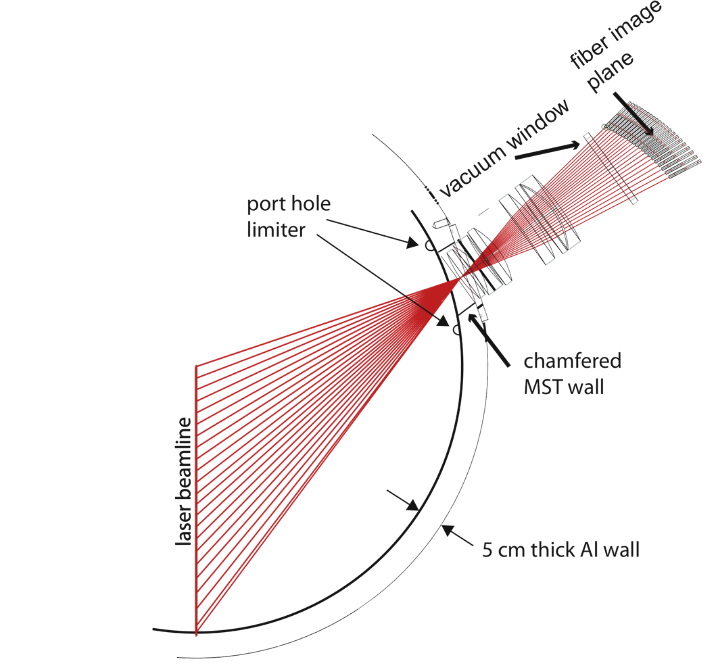
\includegraphics[width = 0.9\linewidth]{./implementation/diagnostics/ts_optics_diagram.png}
	\label{fig:ts_optics_diagram}
	\caption[Diagram of Thomson scattering optics and sight lines]{Diagram of Thomson scattering optics and sight lines. The scattering angle in equation \ref{eq:Sheldon} are dictated by angle made by the red view paths and the laser beam line. (Reproduced from J. Reusch.\cite{Reusch2011})}
\end{figure}

In MST, the TS diagnostic has 21 sight-lines. The scattering angle for a particular sight-line is fixed by the geometry of the viewing optics and ranges from $\sim 108\degree$ to $\sim 143\degree$. The wavelength dependence is observed via an array of polychromators equipped with avalanche photo-diodes digitized at 100MHz to help separate the scattered laser light from the background (digitized both before and after the laser pulse). The temperature $T_e$ is found via least \chisq\ fitting of these observations. The temperature measurements are localized by the intersection of the laser beam path and the viewing geometry, allowing direct $T_e$ profile measurements without relying on inversion techniques. The main limiting factor of TS diagnostics are the fact very little of the incident beam power is scattered (ie. the cross section is very small), and thus it relies on a very powerful pulsed laser (pulse energies $\sim$ Joule) to provide the incident beam. Such lasers are often limited in their repetition rate due to the technical difficulties with heat in the lasing medium, thereby limiting the ability to diagnose fast phenomenon. MST's TS system is powered by two laser ``backends.'' The older ``work-horse'' system is based on a pair of off-the-shelf Q-switching Nd:YAG lasers operating at 1064nm. A series of upgrades have been made to the Pockel cell drivers (that are responsible for Q-switching) and power supplies that significantly increase the repetition rate achieved to up to $\sim 1$~kHz per laser over $\sim 15$~ms of active time\cite{DenHartog2010}. In standard operation, the two lasers' timing are staggered in such a way to achieve effectively a 2~kHz pulse rate. This is the mode used to take the data related to this research, as it focuses more on the slower time scale effects the electron $T_e$ have on the ions. The effective TS frequency of 2~kHz affects the rate at which the plasma kinetic profiles are updated and sets the evolution timescale of the model. This issue will be addressed in more detail in section \ref{sec:time_blocks_and_steps}. For studies of faster plasma phenomenon, the Spectron lasers can also be operated in a pulse-burst mode\cite{DenHartog2010} where bursts very fast pulses are produced and repeated. A typical repetition rate in this mode produces 8 pulses at 25~kHz, and these bursts themselves repeats at 1~kHz. The TS system also has an alternative custom-built laser system commonly called the Fast Thomson system despite the fact that the `regular' TS system is already very fast. The Fast Thomson system can be operated at a repetition rate of up to 333~kHz for 3-4 pulses, or 100~kHz for 44 pulses\cite{Young2015}, giving it exceptional capabilities to resolve fast $T_e$ dynamics. It is, however, not relevant this this work. 

A detailed overview of MST's TS system can be found in the thesis of J. Reusch\cite{Reusch2011}, and an recent comprehensive treatment of TS theory is available by Prunty\cite{Prunty2014}.


\subsection{Ion Doppler and charge exchange recombination spectroscopy}\label{sec:ids}

Naturally occurring ion line emission in the plasma due to electron impact excitation and charge exchange with recycled neutral deuterium, is shifted in wavelength by ion velocity due to the Doppler effect and broadened due to the the thermal velocity distribution of the plasma ions. The broadening occurs since a portion of the observed line emission is red-shifted due to ions having velocity away from the observer and an portion is similarly blue-shifted. A net flow velocity in the plasma causes a net wavelength shift. Spectrally resolved measurements of this line emission can be observed using a spectrometer to determine the emitting ion population's density, velocity, and temperature.

\subsubsection{Physics principles of IDS}
The emission lines used to make theses observations can come from one of three reactions: electron impact excitation, charge exchange recombination, or radiative recombination. For the range of plasma temperature and density achieved in MST, %and in fusion physics in general, (This is not true for a detached diverter for example)
the radiative recombination is a negligible contribution. Typical line emission from MST consist primarily of the result of electron impact excitation and neutral deuterium charge exchange reactions with impurities. The impurities themselves are either atmospheric contaminants (like oxygen) or sourced from limiter sublimation (carbon) and wall sputtering (aluminum). Since this line emission is naturally occurring in the plasma, only a spectrometer and appropriate viewing optics are necessary to observe the emission to obtain information about the plasma. But ion Doppler spectroscopy using naturally-emitted line emission integrates light emitted from the entire plasma volume along the line of sight which is typically not uniform. This means the measurements are not localized except by the emission shells that form for partially-ionized ions in the temperature gradient regions of the plasma. Interpreting this emission requires detailed calculations of ion charge state which depends on the electron temperature and density as well as the neutral deuterium density and it can be a challenge to interpret measurements made. 

Charge exchange recombination spectroscopy (CHERS, or CER) is a special case of Doppler spectroscopy where a neutral beam is used to stimulate charge exchange emission along its path, allowing the spectrometer to make localized measurements where the beam and line of sight intersects. The Doppler shift due to the line-of-sight velocity of an emitting ion is 
\begin{align}
    \Delta\lambda = \lambda_0 \frac{v}{c}.
\end{align}
If we assume a Maxwellian distribution of emitting ions, then the lineshape of the spectral radiance is 
%altered from the $R(\lambda) = I_0\delta(\lambda_0)$ to 
% Technically, there is always some broadening, no matter how small. Even for very cold ions in atomic traps there is broadening due to quantum mechanical uncertainty effects referred to as "natural broadening."
%--
%Got it. -Xing
\begin{align}
    R(\lambda | v, T, I_0) &= \frac{I_0}{\sigma_\text{th} \sqrt{2\pi}}I_0 e^{\frac{-(\lambda-\lambda_c)}{2\sigma_\text{th}^2}}\\
    &\text{where:}\\
    I_0 &= n_{\text{imp}}n_s \left< \sigma v \right>^* &\text{is the total intensity}\\
    \sigma_\text{th} &= \frac{\lambda_0}{c}\sqrt{\frac{kT_\text{imp}}{m_{\text{imp}}}} &\text{is the thermal broadening, and}\\
    \lambda_c &= \lambda_0(1+\frac{\left< v_\text{imp} \right>}{c}) &\text{is the velocity shifted wavelength.}
\end{align}
Additionally, $n_s$ is the density and $\left<\sigma v\right>$ is the effective reaction rate (with branching fraction modification) of the emission generating reaction, $T_\text{imp}$, $<v_\text{imp}$, and $m_\text{imp}$ are the impurity temperature, velocity, and mass. This equation only considers thermal broadening of the line emission. One advantage that can be seen from this formula is the fact that the 3 plasma parameters of interest can be separated easily for analysis. For example, this thesis uses Doppler spectroscopy to look at impurity temperature, thus absolute calibration of wavelength is unimportant for this work as it effective folds into the $\lambda_c$ parameter. In general, the temperature corresponds to width, velocity to total shift, and density to the integrated radiance. 

Modelling charge exchange requires a bit of special consideration regarding both the isolation of the charge exchange emission, as well as the effect of fine structure broadening. To start, the charge exchange emission observed is contaminated by the same emission line excited through electron impact, referred to as background emission. To extract the local plasma information from the charge exchange emissions, the spectrometer also needs a 'reference' sight-line that looks at (effectively) the same plasma but in the absence of the beam. On MST this is done by having a second parallel sight-line offset about 2~cm toroidally. This way, the background emission can be fitted to a spectrum model and then incorporated into the combined charge exchange and background model for the measurements' sight-line. The second consideration has to do with fine structure of the emission line itself. Ultimately, line emission is the result of a bound electron dropping from one energy state to another and emitting a photon of energy equal to the difference of the energy levels. The energy states associated with primary quantum number $n$ consist of sub-levels due to the interaction of the electron orbital angular momentum with the spin angular momentum. The quantization of the angular momentum introduces the other quantum numbers, $l$, and $s$. Each of the energy sub-levels is also Doppler broadened effectively turning the line emission spectrum into the sum of many Gaussians, known as fine structure. The sub-levels associated with the spin number $s$, is due to Zeeman splitting, and the energy effect is small due to the relatively low magnetic field, and is not significant for the broadening calculations. The angular quantum number $l$ and the energy sub-levels associated have a significant effect on emissions, and charge exchange emissions especially.  Then, it is important to know the relative wave lengths and amplitudes of these component Gaussian emissions. But these can be difficult to calculate analytically as the probability of populating a certain fine structure level is complex and has many dependencies. These calculations have been performed elsewhere\cite{Isler1994}, this thesis instead relies on the Atomic Data and Analysis Structure (ADAS) database for the relative population of the fine structure states\cite{Summers2004}. 

\begin{figure}[!htb]
	\centering
    \begin{subfigure}[t]{0.5\textwidth}
        \centering
        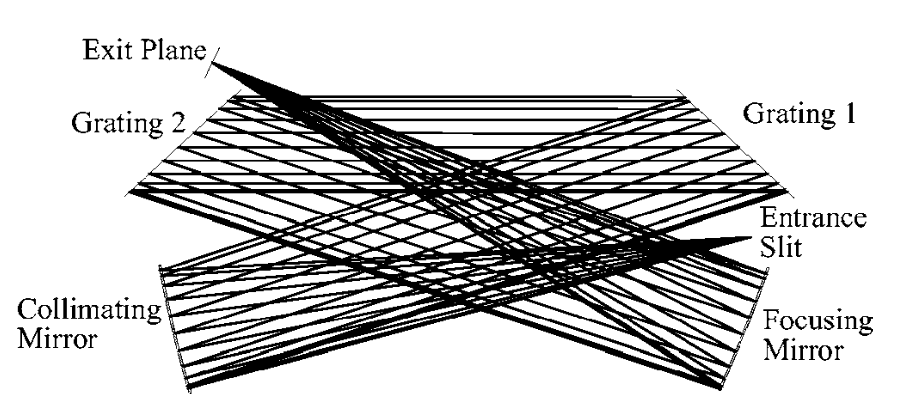
\includegraphics[width = \textwidth]{implementation/diagnostics/idsii_trace.png}
        \caption{Optical layout of IDS-II via ZEMAX}
    \end{subfigure}%
    ~ 
    \begin{subfigure}[t]{0.5\textwidth}
        \centering
        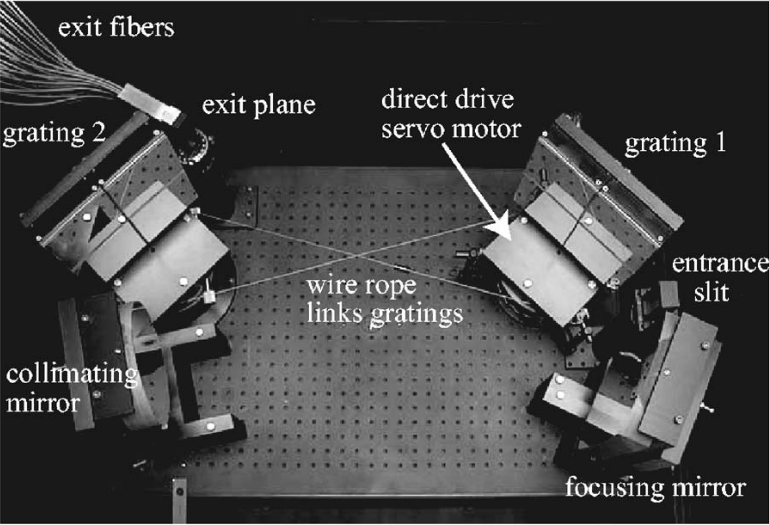
\includegraphics[width = \textwidth]{implementation/diagnostics/idsii_photo.png}
        \caption{Photograph of IDS-II layout}
    \end{subfigure}
	\caption[IDS-II optical layout]{IDS-II optical layout. Reproduced from Craig et al. \cite{Craig}}
	\label{fig:IDS-II}
\end{figure}

\subsubsection{Doppler spectroscopy hardware on MST}
On MST, ion Doppler spectroscopy is performed using the IDS-II (ion Doppler spectrometer, mkII). It is a custom built, high throughput spectrometer optimized for the 343~nm C~VI line, but it could be used for any viable emission line between 200~nm and 480~nm. This spectrometer can simultaneously measure emission from light collected along two optical views, either for the measurement and the reference views used for Charge exchange recombination spectroscopy, or two passive Doppler spectroscopy locations simultaneously. It uses a double grating Czerney-Turner design to achieve a high resolving power ($\lambda/\Delta\lambda \sim 5600$) while each of the gratings are actually a mosaic of 4 gratings, giving an large total area in order to achieve the high {\'e}tendu of 0.40 mm$^2$sr per view(see figure \ref{fig:IDS-II}). It uses a series of photo-multiplier tubes (PMTs) to measure the spectral radiance, allowing the system to achieve an effective data rate of up to 100~kHz in high current plasmas\cite{Craig}. Recent improvements improvements to the frequency response of the transimpedance-amplifiers have allowed fluctuation measurements up to 400~kHz\cite{Nishizawa2016}.


\begin{table}[h!]
    \centering
    \begin{tabular}{||c|c|c||}
        Chord \# & r/a & $\rho_v/a$\\
        \hline 
        1 & -0.91 & -0.92 \\
        2 & -0.76 & -0.80 \\
        3 & -0.58 & -0.64 \\
        4 & -0.41 & -0.48 \\
        5 & -0.24 & -0.32 \\
        6 & -0.07 & -0.15 \\
        7 & 0.11 & 0.03 \\
        8 & 0.28 & 0.20 \\
        9 & 0.45 & 0.37 \\
        10 & 0.62 & 0.55 \\
        11 & 0.80 & 0.75
        
    \end{tabular}
    \caption[IDS-II view chord locations]{IDS-II poloidal viewing chord locations. The $\rho/a$ refers to average magnetic flux surface location in axisymetric plasmas.}
    \label{tab:ids_chord_loc}
\end{table}

The IDS-II system has 11 poloidal viewing chords available, listed in table \ref{tab:ids_chord_loc}. It also has toroidal views available, but they are not used for this project since over the time scales studied the ion temperature is isotropic. 

A diagnostic neutral beam (DNB) is used to inject neutral particles to make localized CHERS measurements. The 'diagnostic' in it's name refer to the fact that the beam current is small such that it does not effectively perturb the plasma being observed, in comparison with heating and fueling beams that are designed to increase the temperature and density of the plasma. The DNB on MST is a nominally 50 ~keV, 4~A hydrogen neutral beam with a pulse length of 20~ms\cite{Feng2016}. The beam energy is optimized for the C$^{6+}$ charge exchange emissions which has a peak reaction rate at 45-50~keV. The beam has recently undergone a refit and the beam composition is measured to be about 75\% at full energy, 20\% at half energy and 5\% at a third energy.\cite{Feng2016}

\subsubsection{Line fitting and ensemble analysis}

This work uses the CHERS data obtained in two different modes and a brief discussion of the line fitting and ensembling techniques is needed to place them in context. The raw signals from the PMTs are digitized at 1MHz, but as discussed above, the spectrometer is designed for data-rates up to 100kHz; the difference is account for in the analysis algorithm. A linearized fluctuation analysis technique alternative to the one described here has been developed to analyze fluctuations up to 400kHz\cite{Nishizawa2017}, however this work focuses on the slower dynamics of the quai-equilibrium values and does not use this alternative. The default method starts by converting the 1MHz data into intensity through gain calibration values, then they are summed into time bins at the desired data frequency (1kHz to 100kHz are common), and subsequently, its photon-counting uncertainty is calculated from calibration (described in detail in T. Nishizawa's thesis\cite{Nishizawa2018}). Afterwards, a piece of code calculates the intensity that each PMT channel 'should' measure at a given temperature, velocity, and amplitude, but also accounting for fine structure and instrumental transfer function. A \chisq value is calculated from this model and the actual measurement, and a nonlinear optimization function is used to find the parameters at which the \chisq\ is minimized. If data analyzed is from two passive IDS views, they are fitted independently the same way. However, if a CHERS measurement is being analyzed, then the passive view (the reference) is analyzed as above, and the active view analysis incorporates this result. It does this by adding the passive contribution to the modeled intensity used to calculate the \chisq\ for the active view. Note that the fine structure for the passive emission and the active can be different as they are difference processes, but the instrumental transfer function are dependent on the view not the process. With this addition, the \chisq\ for the active channel is minimized and the analysis complete.

%%Hey Mark, this section below is going to change significantly, possibly disappear. 
Ensembling of data across multiple shots are used to improve the uncertainty of the measurements. The uncertainty for a particular fit is calculated using the co-variance of the \chisq as a function of the fitting parameters. In effect evaluating the 'width' of the \chisq well in each dimension. If the plasma conditions are perfectly repeatable within the ensembled shots, then the uncertainty of the ensemble can be calculated as the uncertainty of the mean, ie. $\sigma_{\text{ens}} = \frac{\Sigma \sigma}{\sqrt{N}}$. However, the shot to shot variation is not insignificant and the total uncertainty presented is $\sigma_{\text{ens}} = \sqrt{ (\frac{\Sigma \sigma}{\sqrt{N}})^2 + \sigma_{\text{shot to shot}}^2}$, and the shot to shot variation is characterized by the standard deviation of the average ion temperature during the PPCD period of each shot in the ensemble.

This method of uncertainty estimation is appropriate for the relatively slow 10kHz fits used for the model comparison work. However, the m = 0 burst analysis presented in chapter \ref{ch:m0} uses fast 50kHz fits, ensembled over m = 0 burst events. The shorter integration time used for the faster fitting means that each fits are noisy enough that sometimes the \chisq 'well' is poorly formed. Also, the burst to burst variation can be large and changes over the burst period. Hence, the uncertainty on the bursts are presented using the upper and lower values that bounds a 67.8\% of the points in the ensemble (\textit{i.e.} 1 sigma). This is chosen instead of the standard deviation value during the burst itself, the distribution of temperature values of a particular ensembled 'bin' tends to be skewed. 


%==section on modeling methods==
\section{Modeling Methods and assumptions}
In addition to the diagnostic inputs, there are various details of how the model is put together that serves to inform the discussion of the results. These topics include data selection and ensembling, equilibrium reconstruction, and similar modeling considerations, as well as the particulars of the initial conditions and boundary conditions. 
%%% The above statement doesn't really say much. Hopefully you are providing the right level of detail throughout all of your writing :) -- MDN
%----
%Noted, removed statement. -X

\subsection{Shot selection criteria and ensembling of diagnostic inputs}

The modeling work revolves around the ion transport in well-behaved PPCD periods. Data from the PPCD periods included in the ensemble are selected according to the following criteria:
\begin{itemize}
\item periods with little or no burst activity as determined from magnetic fluctuations and poloidal gap voltage measurements; 
\item early onset of enhanced electron confinement (12~msec or earlier) determined by a systematic rise in soft x-ray emission;
\item density and current approximately in range of the rest of the shots used ($n \approx 0.7 \times 10^{19} /m^3$ and $I_p \approx 480 - 500kA $) at their peak during the PPCD period;
% Specify the density and current ranges used to select shots. Is the initial density 5 \times 10^18 m^{-3} \pm 10^18 for instance? 
%----
%Clarified -X
\item reliable operation of the interferometer and Thomson Scattering diagnostics.
\end{itemize}
The ensemble of ion temperature measurements are drawn from CHERS data from a larger set of shots. The spectrometer gives single-point measurements and building up an ensemble of data to reconstruct the evolution of the ion temperature profiles requires many more shots. These shots are chosen by the same criteria as listed above, but the ensemble includes days where the FIR interferometer and Thomson Scattering diagnostics are unavailable.


\subsection{Equilibrium reconstruction through MSTfit}\label{sec:MSTfit}

% To which code are you referring here? It's not quite clear in the context of the Chapter.

% You also need an introduction to what is entailed in an "equilibrium reconstruction," and what is MSTfit. You are assuming that all of the relevant ion heat transport processes operate on the radial transport time scale. Transport along field lines (and within flux surfaces) operate by ions streaming at the thermal speed along a field line. This process is considered fast enough to equilibrate the ion distribution function within a flux surface. The question then becomes, what is the geometry of the magnetic flux surfaces and what is the temperature and density on each of the nested flux surfaces. Since the ions are equilibrated quickly within flux surfaces, the only remaining pressure gradient is in the radial direction. Write down the radial pressure balance equation, assume that the magnetic field and current density can be written in terms of flux coordinates, and then you have the Grad-Shafranov equation. MSTfit solves the Grad-Shafranov equation constrained by the available data from the diagnostics described above. Your ion heat transport model makes use of iterative solutions of the Grad-Shafranov equation to determine changes in the ion heating and cooling mechanisms over transport time scales.
%----
%Noted, Currently correcting. -Xing
As discussed in the previous chapter, the 1-D model relies on the fact that the transport within flux surfaces are well equilibrated on the time scale of interest, and relatively well formed compared to standard RFP plasmas. Plasma parameters, with exceptions of neutral calculations, are thus treated as flux surface quantities in a cylindrical approximation. The determination of the quasi-equilibrium magnetic geometry is done by a process referred to as equilibrium reconstruction through the MSTfit code. Given a set of magnetic, density and temperature measurements, MSTfit uses a non-linear solver to find the best fit 2-D solution to the Grad Shafranov equation:
\begin{align}
    J_(\phi) &= \frac{2\pi F F'}{\mu_0 R} + 2\pi Rp'
\end{align}
where $F = RB_{\phi}$ and $p$ is the pressure, assumed to be isotropic. The reconstruction code further assumes a symmetric plasma, which is well suited for PPCD. In doing so, the FIR measurements of density and internal magnetic field, as well as Thomson Scattering measurements of $T_e$ are used as part of the constrain data. The details of how this is achieved can be found in J. Anderson's thesis \cite{Anderson2001} and paper \cite{Anderson2004}. The result of this process is a set of flux surfaces with associated temperature and density, as well as associated magnetic field.  Because of this, the electron density measurement is not of an independent inversion of line integrated measurement, but a part of the non linear fit; same applies to magnetic field and electron temperature. 

The transport model takes advantage of this existing code base by reading these information as input. To cover the entire period of interest, as series of MSTfit reconstructions are produced. In order to conduct ensemble analysis, the input diagnostic data is ensembled across the list of shots and then the series of reconstruction is produced for the code. Each of theses fits corresponds to what I term time blocks, the larger time scale of model propagation usedfor the input of plasma parameters. The actual propagation of the model occurs over two time scales. I distinguish the two with the names of time \textit{blocks} (the larger, slower steps) and time \textit{steps} (the smaller, faster propagation steps). 


\subsection{Time blocks and time steps}\label{sec:time_blocks_and_steps}

The model is associated with two pertinent time step sizes. The model code is flexible in what size these steps sizes are for a particular analysis, but for the analysis in this work they are set at ~ 0.5ms and 1$\mu s$ respectively. The slower timescale already mentioned above is the one use for updating the magnetic equilibrium and associated input plasma parameters via MSTfit as well as neutral calculations via DEGAS2 simulations. The PPCD quasi-equilibrium being considered are very stable and slow evolving. The electron temperature confinement time has been previously evaluated to be ~10ms\cite{Chapman2001} and ion confinement is expected to be similar or better, where as the transient nature of PPCD causes the $T_e$ to approximately double in 10ms, setting the effective time scale. Fast dynamics such as turbulence are only relevant to the physics scope of the model in time averaged sense. Hence the ~0.5ms update timescale is sufficient to capture the relevant changes in plasma parameter. Reduction of time block size would involves trades offs with resource requirements, such as needing faster TS data collections rate and thus less overall coverage, as well as more DEGAS2 simulations that significantly impact model run time. As the results in chapter \ref{ch:results} bears out, the power terms being considered for the model, as well as measured $T_i$ also evolves slowly compared to the time block size.

The model calculations are done at a faster timescale that I call time steps. This is set at $1\mu s$ in consideration for numerical error in finite time step propagation. As mentioned in section \ref{sec:transport_summary}, the mathematical core of the model is an numerical integration in time. A rectangle-rule integration is used to simplify the various power term calculations, but it has a relatively high numerical error. The error bound by rectangle-rule integration has an upper bound of 
\begin{align}
    \text{Error} &\leq \sum_{i = 0}^{N} \frac{f'(t_i)\Delta t^2}{2} \leq \frac{N}{2}\text{Max}(f')\Delta t^2 = \text{Error}^*
\end{align}
where t refers to time. With a setting of $\Delta t = 1\mu s$, the percentage error bound,
\begin{align}
    \text{Error}^*_P = \frac{\text{Error}^*(\int f(t))}{\int f(t)}
\end{align}
where $f(t)$ refers to the $\partialt E_{\text{thermal}}$ function as defined in section \ref{sec:transport_summary}, comes to $\approx 0.1\%$. This is due to the low rate of change in the energy function as compared to step size. Of course the verification is performed after the analysis, but conceivably the time step does not need to be so small. 




%The most basic is what I term a time \textit{step}, this is set arbitrarily %%% I would caution against saying that the shortest time step you chose was arbitrary. I think that this time step serves as an interpolation 
%at 1$\mu$s which is much faster than the time scale of the physics under investigation. The transport model terms themselves are calculated (or in the case of the neutral modeling discussed in the next sections, interpolated) per time step, and can smoothly evolve in time. The fine timescale is sufficient to minimize the error and instability associate with finite element (time, in this case) approximation.

%%% Each of these reasons are really only superficial to your analysis. Indeed, you are limited by the rate at which Thomson scattering data are acquired and the frequency with which you perform equilibrium reconstructions. The plasma doesn't care about these limitations, however. The more fundamental question is how quickly does the magnetic equilibrium and the temperature and density profiles evolve? There is already existing work showing that the electron energy confinement time in standard RFP plasmas is about 1 msec and in PPCD plasmas is about 10 msec. Since we expect the ions to be better confined than the electrons, we expect the ion heat transort term to change no faster than the electron transport. Therefore transport losses should be adequatly modeled using a time block of 0.5 msec. Each of the source and sink terms in the ion energy balance equation are expected to evolve on a timescale no faster than this as well since we are eliminating data from any discharges that have burst activity which introduces rapid heating on a shorter timescale (about 100 microseconds). After justifying how fast to expect the different source and sink terms to vary, you can then justify the data acquisition rate for the different diagnostic measurements used for the ion heat transport model and the time step over which to evolve the model.

%The first is that MSTfit, in it's standard configuration, takes data inputs from a 0.25ms window for it's equilibrium reconstruction. Since the input data is an ensemble of shots, it is conceivable to run MSTfit calculations with a smaller window more often, it is not a particularly urgent concern as the model is aimed to capture faster time scale physics, and the PPCD plasmas themselves do not contain physics that would show themselves in a somewhat faster tempo of equilibrium reconstruction. The more important constraint on the time block size is the data-rate of the Thomson Scattering diagnostic at 2kHz. $T_e$ is an important input that helps MSTfit determine the pressure term in equilibrium reconstruction. If the TS measurement is unavailable, MSTfit uses a mock $T_e$ profile based on plasma current, but it is insufficient for high current PPCD plasmas. If a mixture of MSTfit reconstructions, some with and some without TS measurement of $T_e$ is used for the model, then an unacceptable amount of 'wobble' in the reconstructed flux surfaces would occur as the model goes from a TS based reconstruction to a TS free reconstruction. Similarly, as the interpretation of both the FIR interferometry and polarimetry measurement is aided by the flux surface reconstruction, it does not make sense to try to incorporate those at a higher frequency either. Again, the result of simple inversions of line integrated FIR measurements is sufficiently different from those aided by equilibrium reconstruction that it would detract from the model. Finally, the DEGAS2 neutral simulation (section \ref{sec:DEGAS2}) also depends on the $T_e$ profile significantly. Thus, then only diagnostic that meaningfully independent of TS's timescale is the charge exchange measurement of $T_i$, which serves as a comparison to the model's predictions. However, despite the fact that diagnostic inputs are made available to the model via MSTfit every time block, they are spline interpolated onto the smaller time steps to avoid sudden jumps in profiles.

\subsection{Monte-Carlo neutral simulation through DEGAS2}\label{sec:DEGAS2}

As mentioned in section \ref{sec:dalpha_array}, the neutral dynamics are more difficult to ascertain than the physics of the $\dal$ emissions would suggest. This is because the neutral density drops very significantly towards the core of the plasma such that it contributes a negligible portion of the $\dal$ emission observed. Simple inversions are not able to determine the core neutral density effectively, especially for PPCD plasmas where the neutral density and resulting $\dal$ emission levels are significantly lower than in standard plasmas. At the same time, although the low neutral density results in insignificant light emission, this does not mean that it can be ignored. Even though the neutral density is a tiny fraction of $n_e$ ($~1\times 10^{-4} to 1\times 10^{-5}$), the charge exchange reaction of this low density gas with ions in the hot core is an important heat transport channel. To asses the neutral dynamics and how it effects the ion thermal transport, a Monte-Carlo simulation is needed. A Monte Carlo neutral simulation initializes a large number of test particles and tracks their behavior though the plasma in physics-based probabilistic calculations. Net characteristics of the neutral population can then be tallied though the net behavior of all the test particles. Monte Carlo simulation are the standard for neutral dynamic calculations since the neutral mean free path is too large to justify a fluid approximation. Additionally, the neutral population does not necessarily satisfy the same symmetries as the charged particle populations (poloidally-symmetric flux surfaces for example). Unfortunately, Monte Carlo simulations are costly in terms of computing power, and are the calculations that set the pace for the model calculation time. 

The Monte Carlo simulation code used for this work is DEGAS2 developed at PPPL\cite{Stotler}. It is a 2-D simulation that takes 2-D $T$ and $n$ profiles as input and tracks and tallies charge exchange, ionization, recombination, and molecular disassociation reactions, as well as associated particle and heat flow of test particles. For this work, it is setup with 3 source terms at the edge of the plasma (details on their geometry are presented in section \ref{sec:neutral_source_geometry}) and synthetic $\dal$ emission detectors to predict measurements made by the $\dal$ array on MST. The detailed physics of sputtering, recycling, and sublimation underlying the neutral source from the different wall and limiter materials are outside of the scope of this work. The simulations are run such that neutral molecules enter the plasma at a defined rate and geometrical extent, they evolve into different charged and neutral species according to the appropriate rate coefficients, the neutral and charged particle populations are tallied, and the radiance observed by the synthetic detectors is predicted. The neutral source rates are used by the broader model as fitting parameters used to achieve a fit between the predicted $\dal$ emission and the observed data. Conveniently, DEGAS2 tallies quantities of interest such as charge exchange ion loss (a neutral source), particle source rates, and energy associated with ionization directly, which means the model takes the 2-D output of these value and incorporates them via flux surface averaging. While the neutral profiles are \textit{not} flux surface quantities, the ion population travelling around the flux surface will experience the averaged effects from the neutrals, justifying the  assumption of toroidal symmetry.

DEGAS2 simulations are run for each time block (defined in the section previous) as a compromise between both due to  it's computational cost, as well as the availability of $T_e$ measurements, a very important input parameter. This arrangement has one problem, however, and that is model self-consistency. To run DEGAS2 simulations, the $T_i$ profile is needed, but for the ion heat transport model to calculate $T_i$, it needs the outputs from the DEGAS2 simulation. To alleviate this issue, the predictor and corrector method is used.

\subsection{Pseudo-self-consistency, and predictor and corrector methods}\label{sec:predictor_and_corrector}

In addition to the problem of self consistency, it would be advantageous to take into account the time variation of the neutral density profile $n_0$ and source and sink terms (like $P_{CX}$) that vary during a time block rather than modeling their values as suddenly jumping at time block boundaries. This is a concern for adequate physical accuracy both for the direct interactions between the deuterium ions and neutrals and also for the impurity charge state ratio calculations which depend on $n_0$. The impurity charge state affects density and pinch flow calculation which in turns impacts the heating terms, all of which are calculated on a time step basis. A sudden jump in the modeled neutral density profile causes unrealistic time variation of these terms at the time block boundaries. Hence then need to interpolate the power terms for each time step within a time block.

To address these issues the code uses a simple predictor-corrector implementation to propagate transport terms. This method uses the previous time point information as an approximation to 'predict' the following time step, and then uses the 'prediction' to redo part of the calculations and thus correct the values. In general, the predictor corrector method, when applied to explicit methods, can be understood mathematically as the following:

% Why not just write down the predictor-corrector equations for T_i rather than introducing the dummy variable y? Also, I think that this method is called the Euler-Trapezoidal method as you've written it. If the equation for the time derivative of y depended on spatial derivatives of y then it would be called the Crank-Nicolson method. You should note that it is a second-order-accurate numerical method. This should help in determining how short a time block should be.
%--------------
%TO MARK: see below for additions and details on predictor-corrector implementation. I feels like the two time scales bars it from being Euler-Trapezoidal or C-N as the time step propagation is itself just simple Euler. The explanation is hopefully clear, but the notation may be confusing, especially that i and e denotes species. Let me know if it is clear to you. -X
\begin{align}
    y^*(t_{i+1}) &= \Delta t\frac{\partial y}{\partial t}(t_i, y(t_i)) + y(t_i)\\
    y(t_{i+1}) &= \frac{\Delta t}{2} \left(\frac{\partial y}{\partial t}(t_i, y(t_i)) + \frac{\partial y}{\partial t}(t_{i+1}, y^*(t_{i+1})) \right) + y(t_i)
\end{align}
where $\Delta t$ is the time step size, $\frac{\partial y}{\partial t}$ is a known function, and the asterisk denotes estimation. For the purpose of my model, y would represent the $T_i$. The particular implementation with in the model is somewhat convoluted as the model has two time scales and the predictor corrector calculations are not applied to the fundamental stepsize of the model but to the time blocks. We define j as the time step index, and J as the time block index, and further, use the notation that $j_{J}$ represents the j index such that $t_{j_{J} = t_{J}}$ (\textit{i.e.} the time point represented by time step if index $j_{J}$ is the same as the time block of index $J$). Due to the ratio between the time step and time block size, $j_{J+1} = j+500$ and $j_0 = 0$. To simplify the explanation, the other (non charge exchange) power terms which are calculated for each step and not block and do not have self consistency issue introduced by the two time scales, are grouped together in notation as $P_{\text{other}}$ . In order to propagate the model from index $j_J$ to index $j_{J+1}$ (\textit{i.e.} a time block), first the charge exchange term is calculated at the beginning step:

\begin{align}
    P_{\text{CX},{j_J}} = \text{DEGAS2}(n_{i,j_J},T_{i,j_J}, n_{e,j_J}, T_{e,j_J})
\end{align}
Then the model is propagated assuming that $P_{\text{CX}}$ stays constant between index $j_J$ to index $j_{J+1}$ (\textit{i.e. }$ = P_{\text{CX}, j_J}$), because the $P_{\text{CX}, j_{J+1}}$ cannot be calculated with known information. With that, we can 'predict' $T^*_{i,j_{J+1}}$ with:
\begin{align}
    E^*_{j+1} & = \frac{3}{2}n_{i,j_1}kT_{i,j+1}^*\\
    & = P_{\text{other}, j} + P_{\text{CX}, j_J}\\
    \text{for } &j_J \leq j \leq j_{J+1}
\end{align}
with the predictor's result for $T*_{i, j_{J+1}}$, $P_{\text{CX}, j_{J+1}}$ can be calculated via DEGAS:
\begin{align}
    P_{\text{CX},{j_{J+1}}} = \text{DEGAS2}(n_{i,j_{J+1}},T*_{i,j_{J+1}}, n_{e,j_{J+1}}, T_{e,j_{J+1}})\label{eqn:P_cx_pred}
\end{align}
note that with the exception of $T_i$, the other values are diagnostic inputs and are known quantities in the context of the model and thus are not 'predicted' or 'corrected'. This also applies to $P_{\text{other}}$. Now with $P_{\text{CX}, j_{J+1}}$ calculated, next step is to prepare the 'corrector' by splining $P_{\text{CX}, j}$ for the block:
\begin{align}
    P_{\text{CX}, j} &= \text{linear interpolation}(P_{\text{CX},{j_J}}, P_{\text{CX}, j_{J+1}}, (j_{J+1} - j_J) )\\
    &= P_{\text{CX},{j_J}} + (j - j_J)(\frac{P_{\text{CX}, j_{J+1}} - P_{\text{CX},{j_J}}}{j_{J+1} - j_J})
\end{align}
with this calculated, the model propagate the steps from $j_J$ to $_{J+1}$ again for a second pass, with the splined $P_{\text{CX}}$:
\begin{align}
    E_{j+1} & = P_{\text{other}, j} + P_{\text{CX}, j}\\
    \text{for } &j_J \leq j \leq j_{J+1}
\end{align}
Where upon the block is complete and the code moves on to the next block. Further, $P_{\text{CX},{j_{J+1}}}$ has already been calculated (in equation \ref{eqn:P_cx_pred}) and can be used to start the next block. By taking this expedience, DEGAS2 is only ever run with $T_i^*$ (the 'predicted' temperature) as the input, and in theory, additional accuracy could in theory be gained by rerunning DEGAS2 after the $T_i$ calculations are redone, and circle around the 'corrector' loop again. However, this only very marginally improves the calculation as $T_i$ changes very slowly even compared to time block size, and DEGAS2 calculations are generally more sensitive to $T_e$, which is an external input to the model and does not suffer from the same prediction issues. The primary aim of applying this method is to better approximate the $P_\text{CX}$ and $\partialt n_i$ terms which are important for the model results presented in chapter \ref{ch:results}.
% This paragraph would be more readable if the predictor-corrector equation you actually use for T_i would be written above including the dependencies on n_0, P_CX, n_0^*, P_CX^*, and T_i^*.
%----
%TO MARK: See above elaboration on what the code is doing. -X
\subsection{Other considerations}

The model evolves the ion temperature according to the physics described, but to do that it is initialized with $T_i$ from CHERS measurement. However the CHERS measurement chords needs to be interpolated for use on the finer radial grid of the model. 
% You should write out the analytical form for the "alpha model" and perhaps show a plot of the fitted Ti profile for both an alpha model and a spline interpolation.
%----
%I noted the analytical form. The plot is in the works. -AX
A simple profile function for plasma quantities is the 'alpha model':
\begin{align}
    T(\rho) &= T_0(1 - \rho^\alpha)^\beta + T_{\text{edge}}
\end{align}
where $\alpha$ and $\beta$ are fitting parameters. However, it does not fit the measured $T_i$ profile well (see figure \ref{fig:init_ti}). Instead, a free-knot-spline fit is used. Additional constraints are included to make the initial profile more physical. 
\begin{figure}
	\centering
	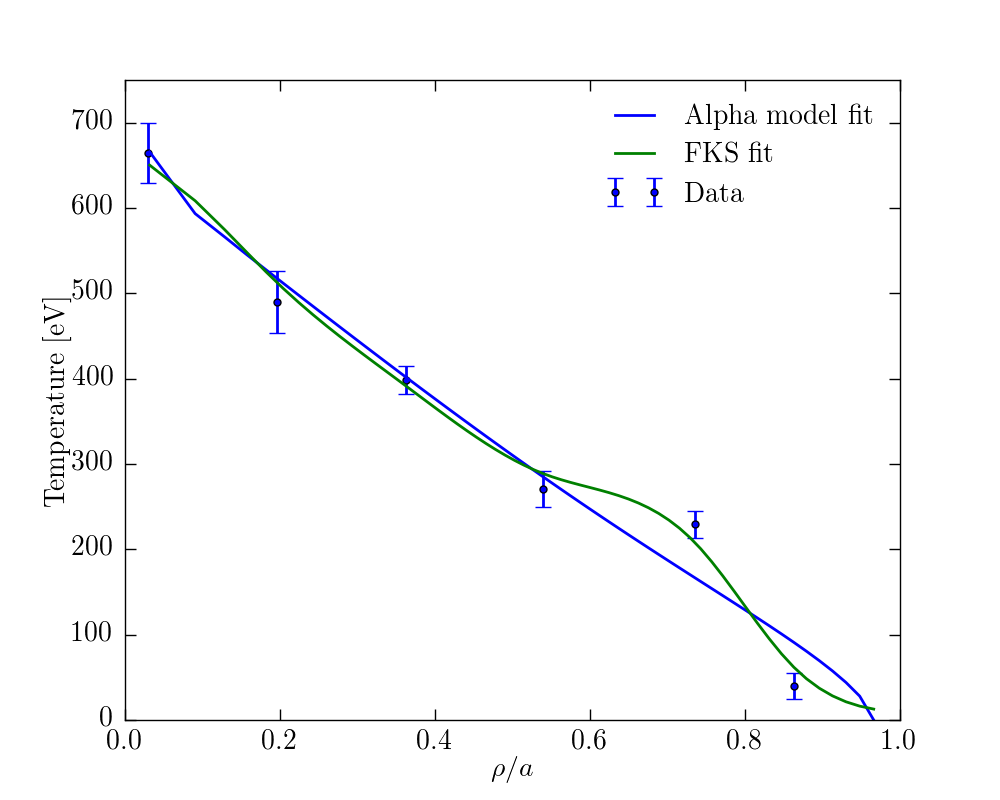
\includegraphics[width = 1.\linewidth]{./implementation/init_ti.png}
	\caption{$T_i$ initial condition and fit.}\label{fig:init_ti}
\end{figure}
% Are you creating this mirrored data in order to provide a Neumann boundary condition of zero derivative at the boundaries?
%----
%TO MARK: yes, I clarified below.
First, the data being fit are mirrored at $\rho_v < 0$ and $\rho_v > a$. This is done to impose Neumann boundary condition, which in turns is important to prevent the edge $T_i$ fit returning a negative region, and is further needed to make sure the very core point (inside the core most measurement) do not get fit to a very high temperature with a gradient. Further, two additional data points added to the CHERS measurements, one is the boundary condition of $T_i(a) = 10eV$, a standard approximation, and the other is the passive IDS measurement of the C-III (C$^{2+}$) emission line in 500kA PPCD plasmas. There are some uncertainty in the location that it corresponds to, and for the purpose of the model this data point is located at $\rho_v = 0.46$, as determined from collisional-radiative modeling of similar plasmas\cite{Nishizawa2018,Barbui2014}. These points are added to the CHERS measurement to arrive at the initial condition because the CHERS measurements by themselves do not adequately sample the ion temperature gradient at the edge.

The boundary condition of the model is largely inherited from the MSTfit reconstruction code \cite{Anderson2001} as it pertains to the input. It is useful to point out that $T_i$ at the edge most location is held constant, and the thermal energy transported to this point is considered lost from the plasma. This is necessary as the MSTfit's boundary condition imposes $n = 0$ at this point, and a temperature cannot be realistically be applied. Similarly, in calculating radial derivatives, the last radial point is ignored and the derivative extrapolated.

Further, quasi-neutrality is imposed on the model. This is to be expected, but it does broach the subject of the role of the impurities in the model. The model does not actively model impurity transport or charge-state evolution; this would be a large extension of the scope of the majority heat transport modelling. However, they are not ignored either. As will be discussed in greater detail in section \ref{sec:eb_pinch}, the radial particle velocity is needed for calculating the flow related terms, and determining the origin of the core density rise. This is calculated by using the particle continuity equation, which in turns depends on the source term and the density change. However, only the electron density is available through measurement, and as the impurities also provide an electron source through ionization, they're effect on the particle continuity equation must be determined. As such, the impurity levels (including carbon, oxygen, boron, and aluminum) are taken from M. Nornberg's work \cite{Nornberg2018}, and added to the model as constant densities with evolving charge state balance. The quasi-neutrality calculation thus includes the impurity contribution, though it is found that their contribution to $\partialt n_e$ is not especially significant in explaining the observed core density increase during PPCD (see section \ref{sec:eb_pinch}).

%\subsection{Basic plasma assumptions}

%\subsection{Role of impurities}


%summary section?

\printbibliography
\end{refsection}
\begin{refsection}


\chapter{Results: Ion Thermal Transport in MST's PPCD plasmas}\label{ch:results}



This chapter describes the main body of results and discoveries made during this modeling effort. Overall, this transport model based on classical effects can adequately describe the temperature evolution in the core, but needs an extra \textit{ad hoc} heating term localized in the edge to explain the edge ion temperature measurements. This chapter will get to this result in three steps. First is a discussion of the neutral dynamics, including the charge exchange and impact ionization rates, in PPCD plasmas. Some unintuitive effects on core neutral dynamics from adding an \textit{ad hoc} heating term in the edge are illustrated. This is followed by a discussion of the inward pinch needed to account for density evolution, how it is correlated with the \ecb flux, its context as part of the net radial flow, and how it affects the thermal transport. Finally, I discuss the comparison between model and data, with and without an \textit{ad hoc} term in the edge. The chosen profile of this anomalous heating term is explained and motivated by proposed physical mechanisms. 


\section{Neutral dynamics in improved confinement MST plasmas}\label{sec:neutral_results}

The neutral dynamics are perhaps the most important factor in ion thermal transport in MST. As explained in previous sections in detail, the neutral dynamics can be difficult to measure directly, and physics-based modeling is needed. The inadequacy of inversion techniques and the need for physics simulation regarding neutrals has already been identified \cite{Eilerman2012}. There have been previous attempts to model the neutrals in MST using a Monte-Carlo simulation code called NENE, based on the principals set out by Hughes \textit{et al.} \cite{Hughes1978}. %Citation for NENE is here: https://doi-org.ezproxy.library.wisc.edu/10.1016/0021-9991(78)90045-1
NENE is similar to the DEGAS2 code that is used for this modeling work.
%How is NENE different from DEGAS2? What did it get wrong? Was it missing important physical processes in the neutral modelling? If so, which ones? Is there a justification for adding a 50eV neutral source in NENE given what you discussed earlier in terms of hot neutrals generated from charge exchange with plasma ions? -- MDN
%Clearified a bit more. --Xing
However, comparatively NENE did poorly for PPCD plasmas, and needed an \textit{ad hoc} 50eV uniform neutral source to improve the quality of fit\cite{Eilerman}. DEGAS2 improves upon NENE by offering a more complete set of physics interactions being simulated, especially around molecular dynamics such as molecular ionization, disassociation, and charge exchange, and well as better accounting of multi-step interactions that adds an effective $n_e$ dependence to impact ionization rate coefficients\cite{Stotler,Janev1984}. Further, the implementation of NENE on MST did not produce neutral temperature information, or the thermal effects of impact ionization, the importance of which becomes clear later in the section. The general setup of the neutral simulation within the model has been laid out previously in section \ref{sec:DEGAS2}, but before the density and temperature results can be discussed, we need to have a short detour to talk about fitting quality and the source geometry used to obtain the fits.

\begin{figure}
	\centering
	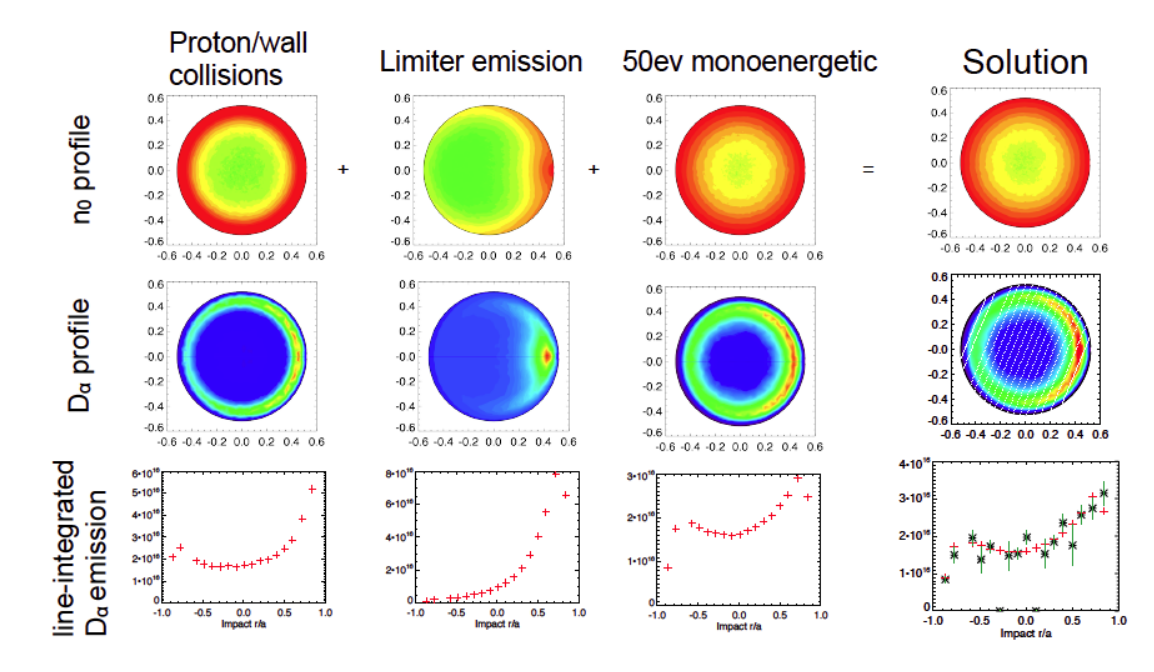
\includegraphics[width = 1.\linewidth]{ion_transport_results/nene_example.png}
	\caption[Example of NENE neutral output]{Example of NENE neutral output, the difference between this and the DEGAS2 results are examined in this section. (Reproduced from S. Eilerman's Thesis \cite{Eilerman})}\label{fig:nene_example}
\end{figure}

\subsection{Neutral source geometry, and fitting of observations}\label{sec:neutral_source_geometry}

In an ideal situation the neutral source rates would be known through direct observation and be modelled using the complete 3D geometry of the vacuum vessel. But as a practical matter, neutral recycling is complex and not within the scope of this work. Instead, a 2D neutral simulation is run with several independent neutral source profiles assuming toroidal symmetry. Each particle source has a defined geometry and rate. An instance of neutral analysis is simulated implementing each particle source independently, and then the rates are linearly fit to the observed $\dal$ emission levels (discussed in detail in section \ref{sec:DEGAS2}). Increasing the number of independent 'sources' via subdividing the wall geometry would give more fitting parameters, but the fitting problem becomes under constrained by the emission measurements, and the computational time needed increases unnecessarily. This work uses a three-source geometry as follows (illustrated in figure \ref{fig:DEGAS2_sources_and_density}):
\begin{figure}
	\centering
	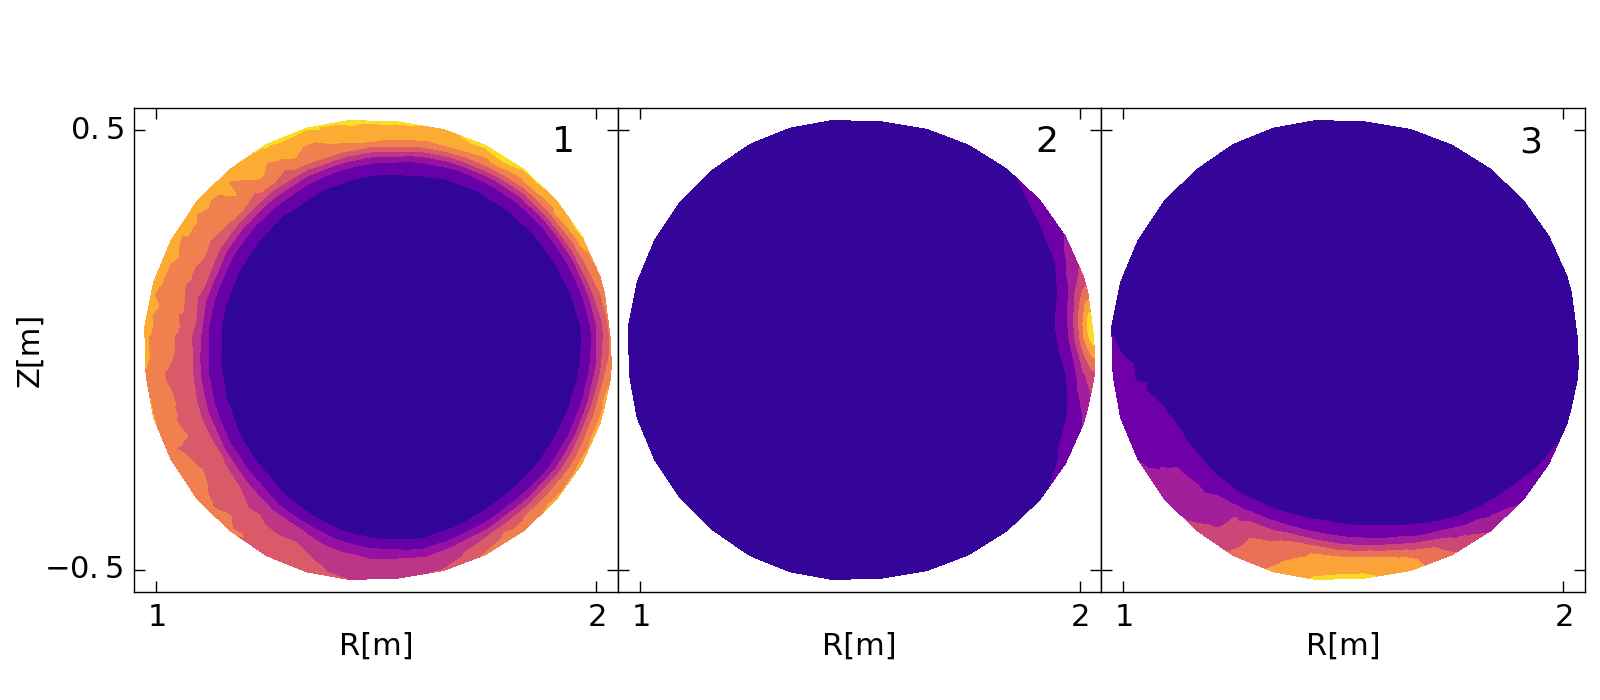
\includegraphics[width = 1.\linewidth]{ion_transport_results/source_comp.png}
	\caption[DEGAS2 source contributions]{Geometry of the normalized neutral density for the 3 sources used in DEGAS2. 1: 'Wall' source, 2:Limiter source, and 3: 'Duct' source. Details in text. It is interesting to point out that in the contribution from the 'uniform' source, there can be clearly observed the effect of the Shafronov shift on the neutral density. \textit{ie.} the neutral density 'hole' is correspondingly shifted to reflect the shift in the ionization region. This phenomenon is not seen in NENE results of the same source (figure \ref{fig:nene_example}), and it is unclear why. Though likely related to self-consistency issues in implementation.}\label{fig:DEGAS2_sources_contrib}
\end{figure}
\begin{enumerate}
    \item A poloidally uniform source representing the walls of MST, with the exception of the area detailed in the following source. 
    \item A poloidally localized source corresponding to the location of the outboard limiter. The outboard limiter (typically) defines the LCFS on MST and is known to be a major source of recycling as well as impurities.  
    \item A poloidally localized source corresponding to the bottom 45\textdegree of the wall. This is the location of the pumping duct and gas injection valves of MST. 
\end{enumerate}
The contributions from each source (to density, for example) are treated as linearly independent. This is due to the fact that neutral-neutral collisions are very rare compared with neutral-ion and neutral-electron collisions at typical parameters. Typical contributions from each source are shown in figure \ref{fig:DEGAS2_sources_contrib}. This project began by considering only the first two sources, with the second extending uniformly around the circumference of the vessel poloidal cross section. However, it is found that in some instances the first two source terms could not be used to explain measurements from the $D_\alpha$ array. In particular, the intensity on the central view chords would be systematically under-predicted by the code. By hypothesizing that the neutral population may have a vertical asymmetry due to preferential sources and sinks in the lower region of the vessel. This is the location of the pumping duct and all of the fueling gas injection valves. If this region has a different effective source rate than 'the rest of the wall', the code is then able to give a better fit to the observations. (see figure \ref{fig:DEGAS2_source_comp})%, and \ref{fig:DEGAS2_typical_fit}). Additionally, it is useful to point out that

\begin{figure}
	\centering
	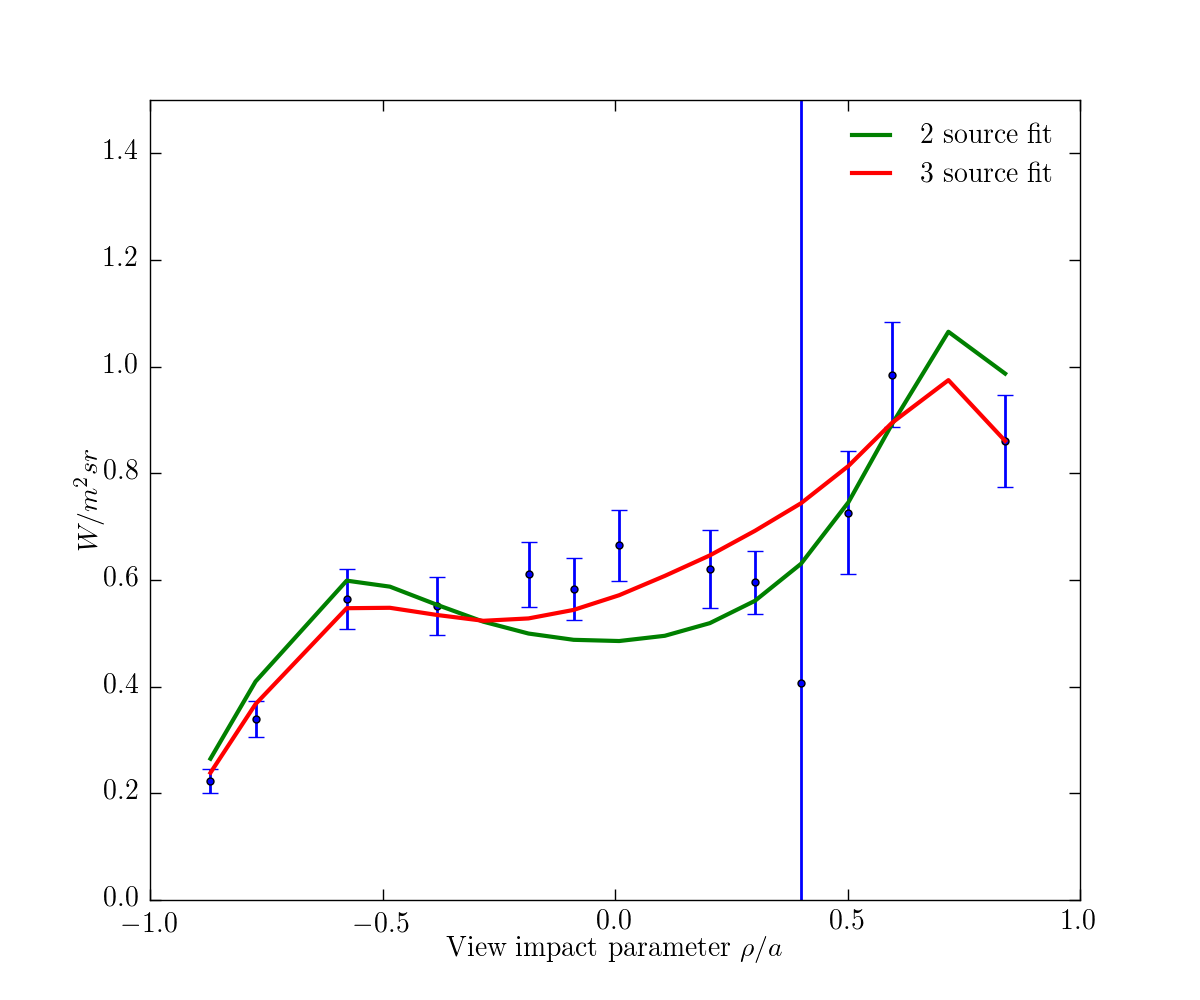
\includegraphics{ion_transport_results/source_comparison.png}
	\caption[Comparison between 2 source and 3 source fit for DEGAS2]{Comparison between 2 source and 3 source fit for DEGAS2.}\label{fig:DEGAS2_source_comp}
\end{figure}

\begin{figure}
    \centering
    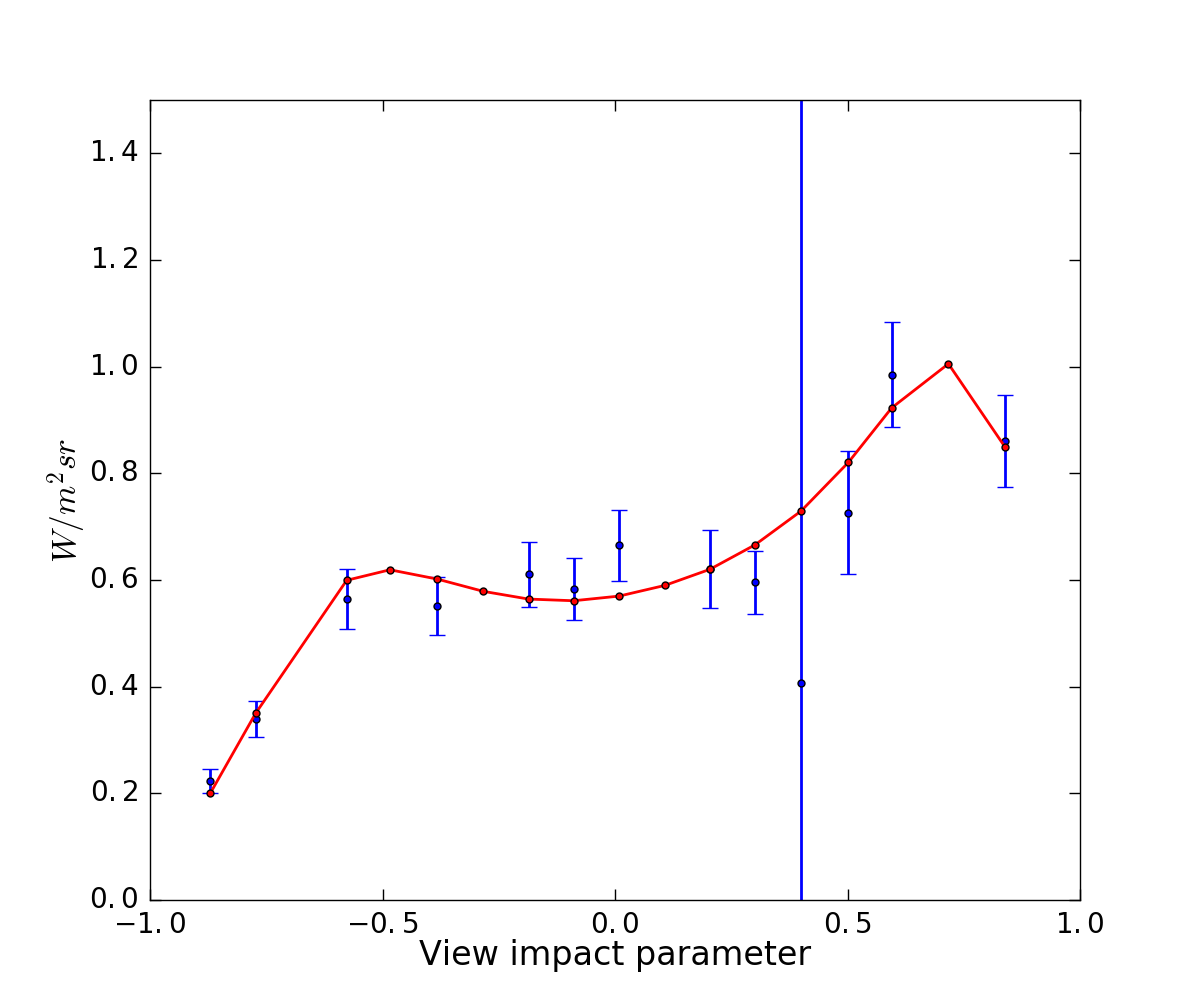
\includegraphics{ion_transport_results/DEGAS2_typical_fit.png}
    \caption{A typical DEGAS2 fit of ensembled $\dal$ signal.}
    \label{fig:DEGAS2_typical_fit}
\end{figure}

\subsection{Neutral density in PPCD}

\begin{figure}
    \centering
    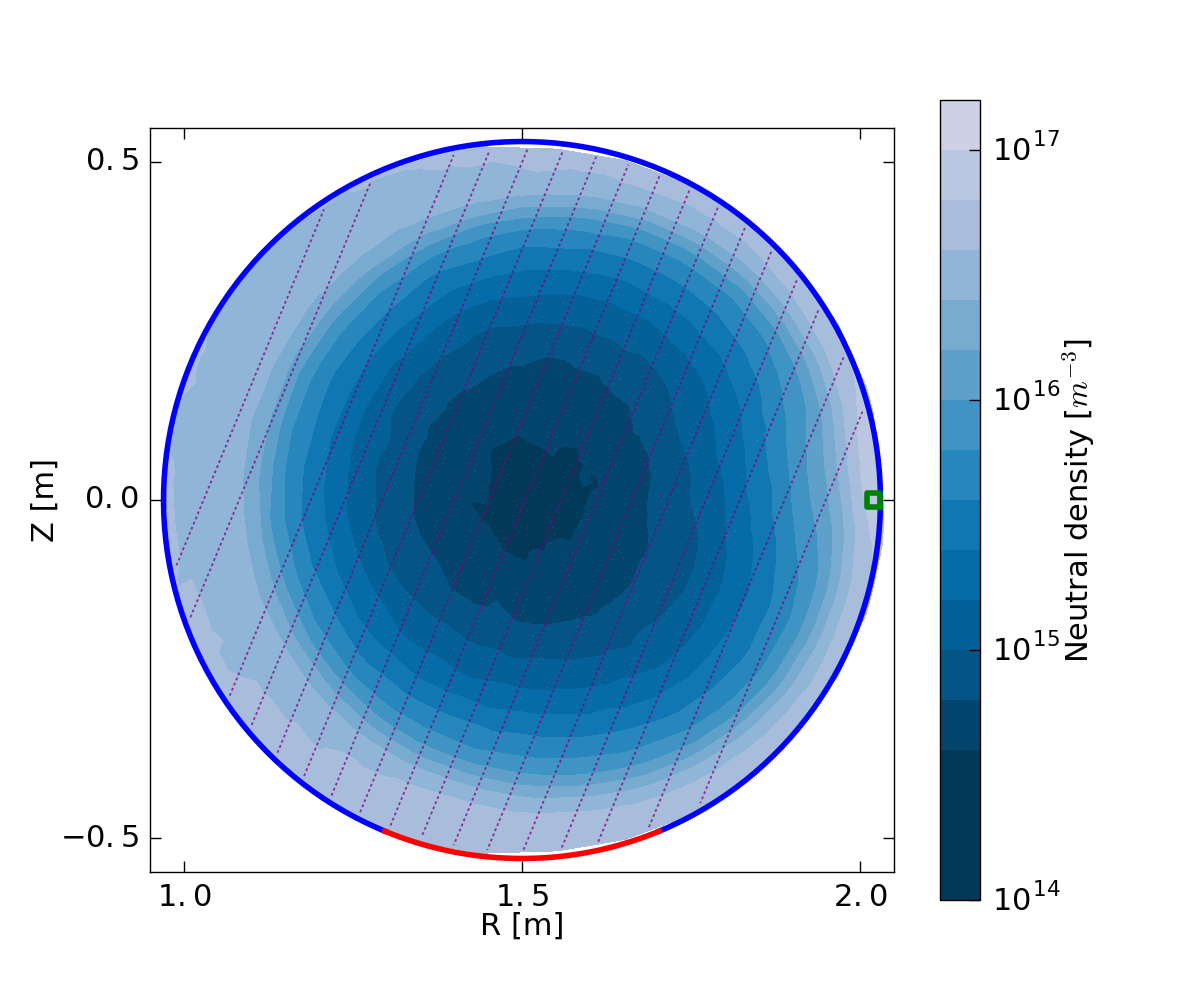
\includegraphics{ion_transport_results/DEGAS2_density2d.png}
    \caption[Neutral density via DEGAS2]{Neutral density via DEGAS2 simulation, with the geometry of the three sources overlayed. Using the numbering presented in section \ref{sec:neutral_source_geometry}: source 1 is in blue, source 2 is in green, and source 3 is in red. The dashed lines represent the location of the available views.}
    \label{fig:DEGAS2_sources_and_density}
\end{figure}

\begin{figure}
    \centering
    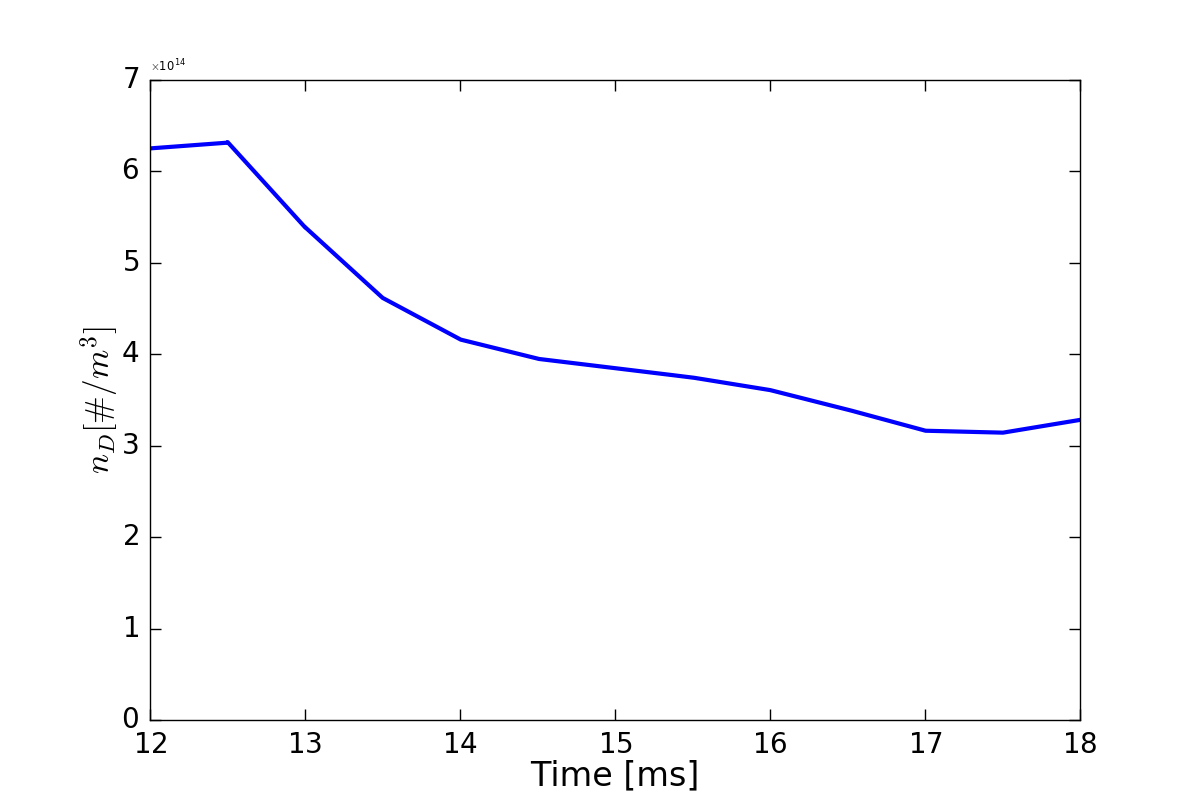
\includegraphics[width=0.8\linewidth]{ion_transport_results/neutral_vs_time.png}
    \caption[Core neutral density over time]{Core neutral density over the time span of the PPCD period. This result is from the ensemble of good PPCD shots analyzed.}
    \label{fig:neutral_vs_time}
\end{figure}

Unsurprisingly, the neutral density is edge dominated and decreases by about 2.5 orders of magnitudes as one 'travels' towards the core. The details can be seen in figure \ref{fig:DEGAS2_sources_and_density} and \ref{fig:DEGAS2_1d}. The edge neutral density is comparable with previous estimates, but the core density is about 1/4 of previous calculations using the NENE code~\cite{Eilerman2010}. % This comparison of the NENE and DEGAS2 code predictions for neutral density profiles that best fit observed neutral emission measurements doesn't really explain which model is more believable. Aside from the ad-hoc 50eV source, what are the differences between the two codes? 
%Added more on the improvement DEGAS2 makes in first paragraph of section. -Xing
Though when NENE is run for my particular shot ensemble, it returns results lower than that presented, and the core density from DEGAS2 is ~ 55\% of NENE. As pointed out above, the DEGAS2 fit have the advantage of not relying on an \textit{ad hoc} 50eV neutral source to achieve the fit, and the neutral density more self consistently show the effect of the Shafronov shift (see also figure \ref{fig:DEGAS2_sources_contrib}). 
Further, the neutral density in PPCD is not entirely constant; the early part of PPCD sees the neutral density decreasing until around 16.5ms when it stabilizes until the end of PPCD (figure \ref{fig:neutral_vs_time}. This neutral density estimates is also in line with that from s. Kumar's measurement of Al charge state fractions in the core. The charge state fraction of Al$^{11+}$ to Al$^{13+}$ is very sensitive to neutral density as the charge exchange process keep the Al$^{13+}$ population down. DEGAS2's estimate of core neutral density. The DEGAS2 neutral density is still too might to match that needed by J. Waksman to explain the NBI heating effects observed. However, this is perhaps not a good direct comparison as his work are on well optimized low current (200kA) PPCD, which, other than the problem of differing plasma current as my parameters, is inherently difficult for $\dal$ observations to constrain neutral density as the emission measurements begin to approach noise levels of the detector. 

\begin{figure}
    \centering
    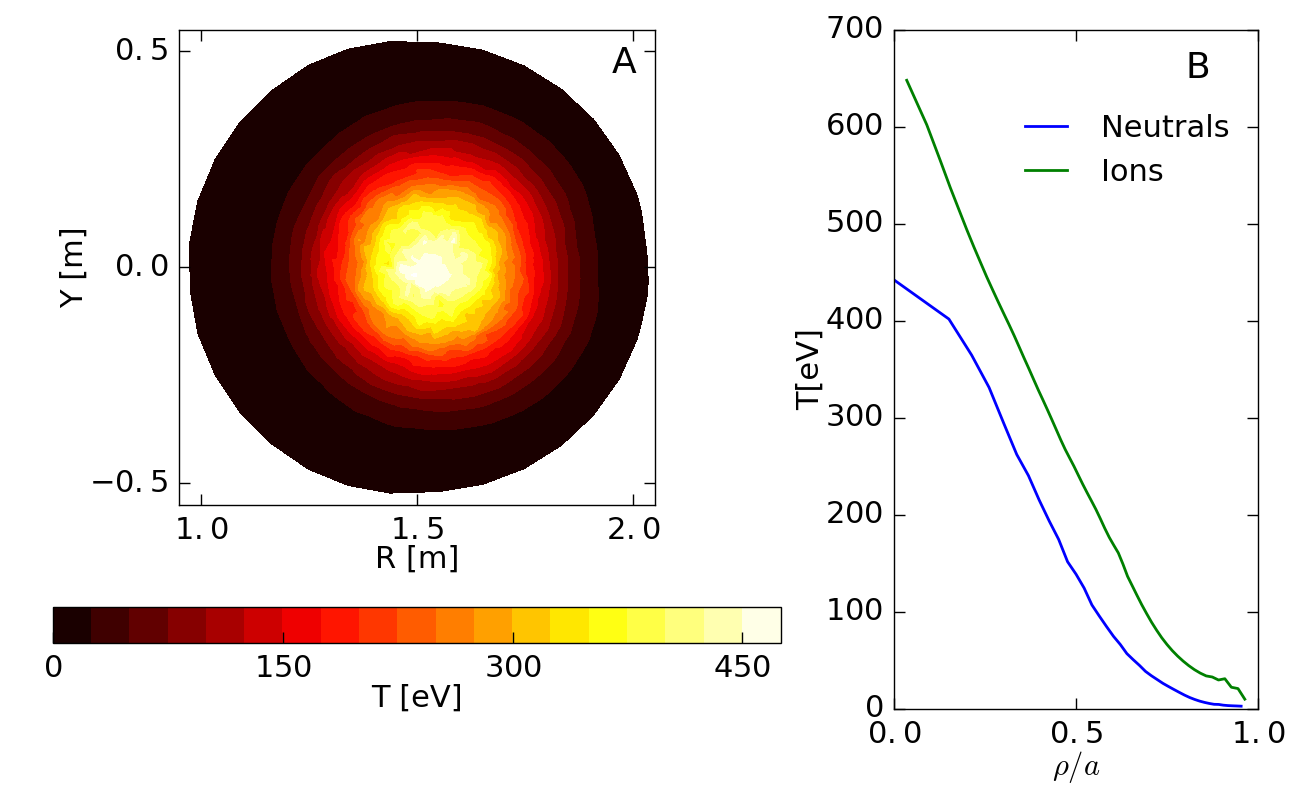
\includegraphics[width=\linewidth]{ion_transport_results/DEGAS2_temperature2d.png}
    \caption[Neutral temperature via DEGAS2]{Neutral temperature via DEGAS2 simulation. A) The 2-d temperature results. B) The flux surface averaged results, with $T_i$ for comparison.}
    \label{fig:DEGAS2_temperature}
\end{figure}

Another notable improvement of the understanding of the neutral dynamics is the neutral temperature information provided by DEGAS2. Though it may not be immediately obvious, but a high $T_{\text{neutral}}$ is needed for the neutrals to penetrate into the plasma volume. The mean free path of a 'room temperature' neutral is very short in MST parameters, and neutrals created by charge exchange reactions, and a small amount of Frank-Condon neutrals from energetic disassociation of D$_2$ would dominate the neutrals interior to the plasma. This is reflected by the DEGAS2 results (figure \ref{fig:DEGAS2_temperature}). Notably, the neutral temperature is a significant fraction of the ion temperature, meaning that only a fraction of the ion's thermal energy is effectively lost in a charge exchange reaction.

\subsection{Charge exchange, impact ionization, and ion source rate}

\begin{figure}
    \centering
    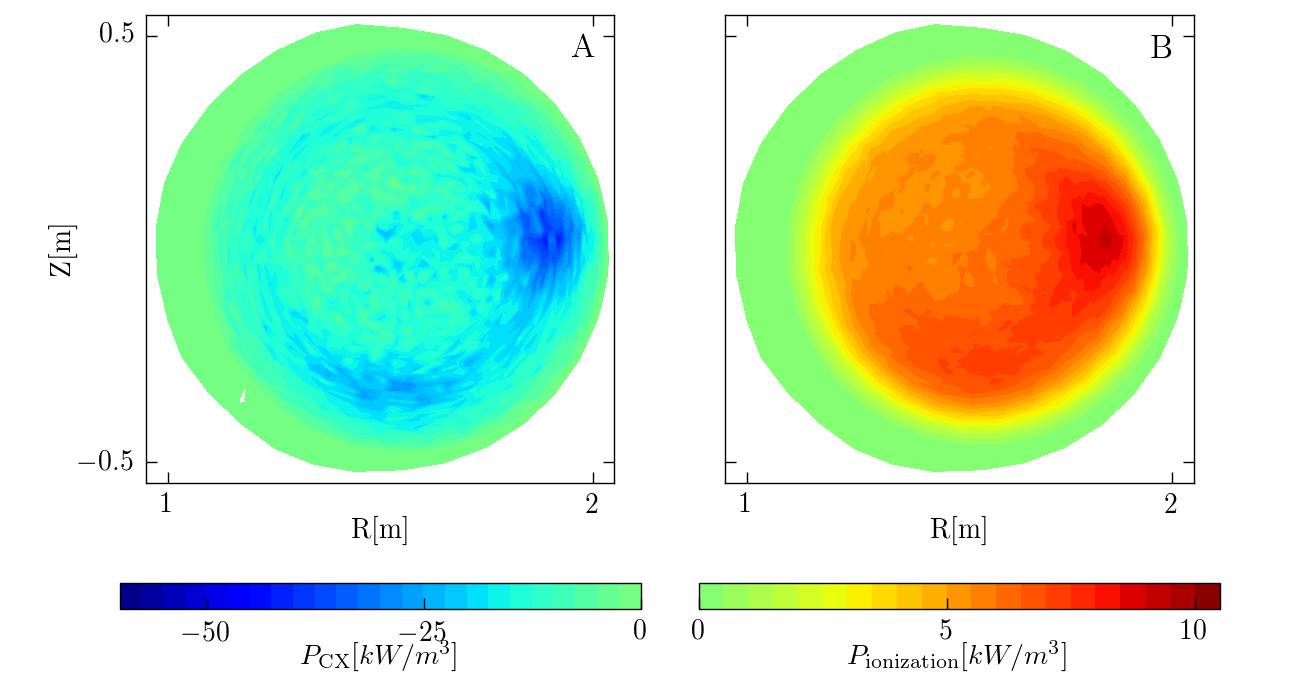
\includegraphics[width=\linewidth]{ion_transport_results/DEGAS2_power_terms_2d.png}
    \caption{DEGAS2 2D  A) charge exchange and B) impact ionization terms. Note the difference in the color bar range. Less obviously, the up/down asymmetry is also present in this plot. This result is from ensembled PPCD shots at 15ms.}
    \label{fig:DEGAS2_power_2d}
\end{figure}

\begin{figure}
    \centering
    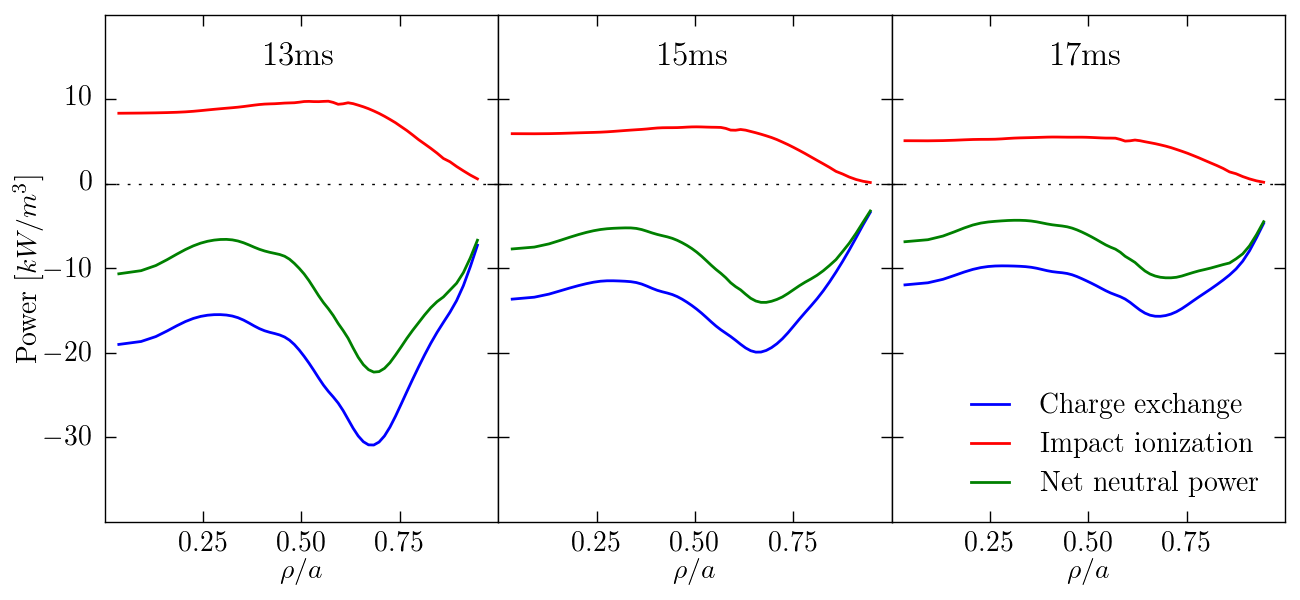
\includegraphics{ion_transport_results/DEGAS2_power_terms_1d.png}
    \caption{1-D neutral power terms at 13ms, 15ms, and 17ms. The 'net neutral power' refers to the sum of the two terms, as electron impact ionization is a process that recovers some thermal energy from the neutrals fluid.}
    %This plot should include 'net charge exchange loss'
    \label{fig:DEGAS2_power_1d}
\end{figure}


The charge exchange loss rate displays an hollow profile that is significantly skewed outboard, like the ion density. However, the poloidal transit time are small on the RFP and neutral effect on the majority ion fluid is still considered on a flux surface averaged basis despite significant asymmetry. On a practical basis, this hollow profile is the creation of the declining neutral density towards the core, and the increasing majority density as well as temperature difference. The trend of declining neutral density also translates to the charge exchange loss as expected. The electron impact heating is an interesting to consider as it represents a partial 'recovery' of the thermal energy lost in charge exchange (details in section \ref{sec:neutral_physics}). However, as the neutral's temperature is below that of majority ion, this actually results in temperature decrease. In general, I use 'heating' to describe thermal energy input into the ion fluid which does not necessarily increase the temperature. 

\begin{figure}
    \centering
    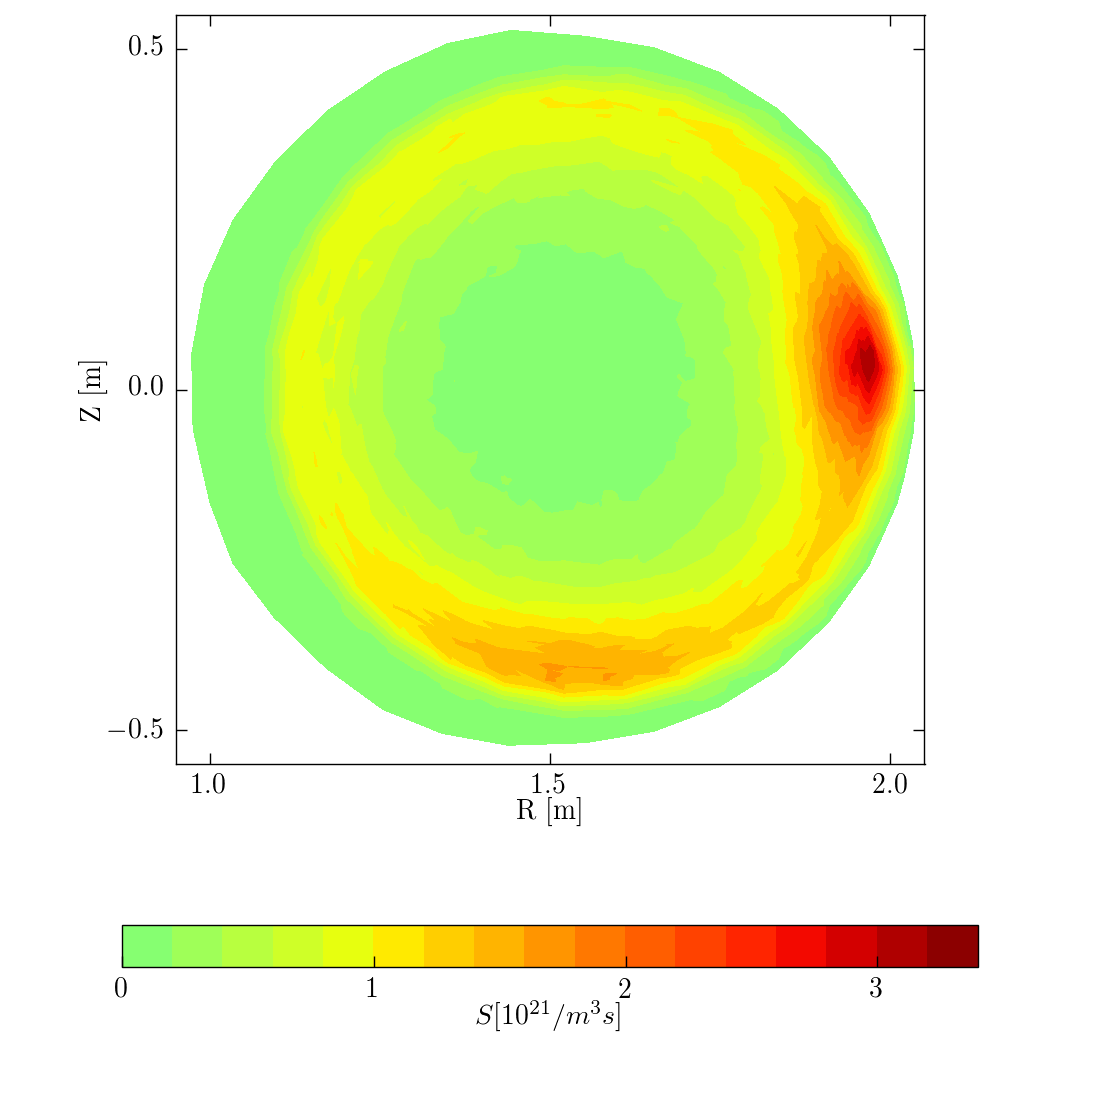
\includegraphics{ion_transport_results/source_2d.png}
    \caption{DEGAS2 ion source rate results.}
    \label{fig:DEGAS2_source_rate}
\end{figure}

The ion source rate also displays the same characteristics as the power terms. However, it is significantly more hollowed out since it does not depend on the difference in ion and neutral temperature, which is higher in the core. This means that the ion source rate is not sufficient to explain the density rise in the core. The consequence of this is to hint at an inward pinch mechanism to be explained in more detail in section \ref{sec:eb_pinch}

%\subsection{Unintuitive model response of \textit{ad hoc} heating in the edge}
%\begin{figure}
%    \centering
%    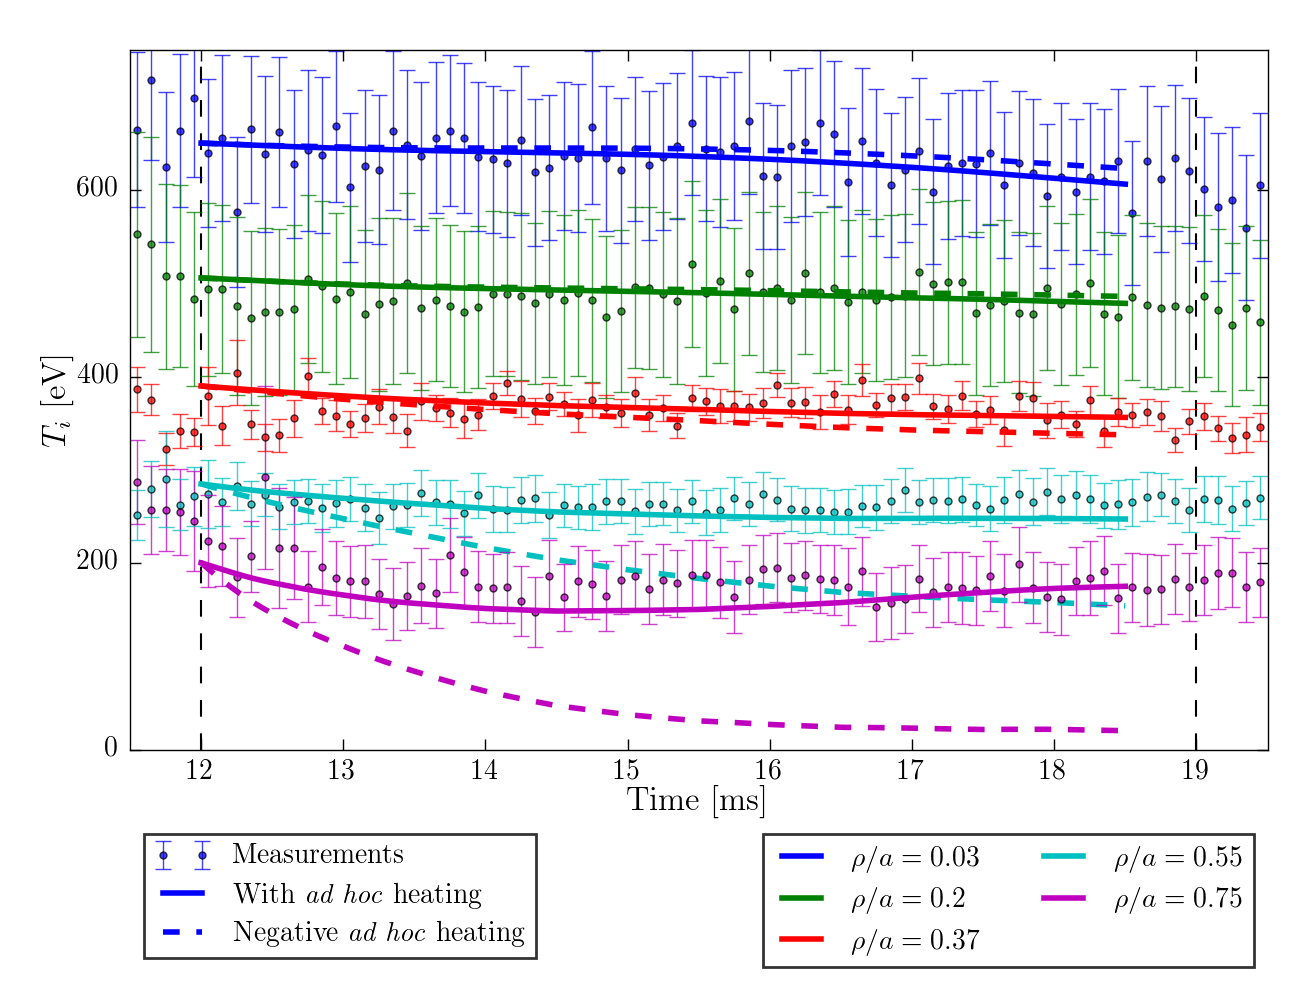
\includegraphics[width=\linewidth]{ion_transport_results/unintuitive_response.png}
%    \caption{The effect of having a low ion temperature edge on charge exchange}
%    \label{fig:unintuitive_cx_response}
%\end{figure}

%During the adjustment process for the model, it became clear that ion heating in the edge have an effect on the charge exchange loss in the core through it's effect on ion temperature. Suppose you have an edge region where the ion temperature is only a few eVs, but the electrons are on the order of 50 to 100 eV. In this region, electron impact ionization of neutrals would dominate charge exchange, and any neutral particle entering the plasma would more likely be ionized before undergoing charge exchange, thus decreasing the neutral penetration. The decreased penetration would in turns result in a more hollowed out neutral density, as well as charge exchange loss and ion source rate. This situation was created in the model from a mistake in the calculation in the flow effects in the edge, and when \textit{ad hoc} heating is applied this erroneous model to bring it inline with the observed temperature without changing how the rest of the model is calculated, the core temperature is predicted to be lower. However, this effect seems most significant when the edge ion temperature drops to ~10eV or lower for a significant radius. When the mistake was corrected, the model predicted edge ion temperature of ~50eV at $\rho_v/a \approx 0.75$ without \textit{ad hoc} heating terms, and increasing it to the observed ~175eV using \textit{ad hoc} heating only dropped the core temperature very slightly.


\section{Pinch in the Reverse Field Pinch}\label{sec:eb_pinch}
%\section{Observations of inward pinch flow associated with $\vec{E}\times\vec{B}$ drift and it's effect on ion thermal transport}

%In previous power balance work, the heat lost to particle flow is one of the largest terms\cite{Fiksel2006}. Calculating $P_{flow}$ involves estimating the ion particle flux.  However, no diagnostic measurements of $n_i$ in MST is available, therefore, $n_i$ is inferred indirectly through the evolution of $n_e$ combined with previous work on characterizing the impurity content in PPCD\cite{Kumar2012,Nornberg2018IncorporatingCharge}.

%...

%Given that the  calculated electron source rates are insufficient to account for the density rise, another possibility is an inward particle flux. The particle flux ($\Gamma_{obs}$) needed to satisfy the continuity equation (\ref{eqn:cont}) is then calculated. However, we seek to confirm the theoretical plausibility of an inward pinch by considering the evolution of the magnetic equilibrium.

%There is currently no diagnostic that measures the poloidal and toroidal $\vec{E}$, which is needed to constrain the radial $\Gamma_{\vec{E}\times\vec{B}}$. Instead, the slow time-scale E field is estimated using the evolution of reconstructed B field from edge flux coil and FIR polarimetry data. The radial flux, $\Gamma_{\rho} = n_e\frac{(\Vec{E}\times\Vec{B})_{\rho}}{B^2}$, is constrained by $E_{pol}$ and $E_{tor}$. The MSTfit equilibrium reconstruction outputs reconstructed flux values and flux surfaces in 2D which enables the calculation of $E_{pol}$ and $E_{tor}$. In particular $E_{pol}$ can be calculated through:

%\begin{align}
%   E_{pol}(\rho_v) & = -\frac{1}{\rho_v}\int_{0}^{\rho_v}\rho_v' \frac{dB_{tor}}{dt} d\rho_v'
%\end{align}

%where it is taken as a boundary condition that the $E_{pol}$ is zero at the magnetic axis.

%where $\rho_v$ is the flux surface averaged minor radius.

%Calculating $E_{tor}$ is slightly more complicated, as it is a function of major radius and not $\rho$. On MST, there is a poloidal gap (a cut in the vessel in the poloidal plane) in the conducting wall and the voltage measured across the gap ($V_{PG}$) is a reflection of the inductively driven toriodal E field. To incorporate into the 1-D approximation, $E_{tor}(R, Z=0)$ along the Z = 0 plane is determined as a function of major radius (R) through:

%\begin{align}
%\oint_S \vec{E}\cdot d\vec{l} &= -\iint \frac{\partial}{\partial t}\vec{B}\cdot d\vec{s}\\
%E_{tor}(R) 2\pi R &= -\int_0^{2\pi}\int_{R_{in}}^{R}R'\frac{\partial B_{pol}}{\partial t} d\phi'dR' - V_{PG}\\
%E_{tor}(R) &= -\frac{1}{R}\int_{R_{in}}^{R}R'\frac{\partial B_{pol}}{\partial t} dR' - \frac{V_{PG}}{2\pi R}\label{eqn:E_tor}
%\end{align}
%where $R$ refers to the major radius, and $R_{in}$ is the major radius at the inboard wall.

%Since the $ \frac{dB}{dt} $ term cannot be evaluated directly, sequential MSTfit reconstructions, 0.5ms apart are used to provide $ B_{pol} $ and $ B_{tor} $ information from which a numerical derivative is calculated. The results show $E_{tor}$ to be relatively stable in the core, but changes direction in the edge as time progresses. This reversal correlates with current drive being exhausted in the edge. Note this is not related to the edge $\vec{B}$ reversal that gives the RFP it's name. From $E_{pol}$ and $E_{tor}$, the radial particle flux is calculated as: 

%\begin{equation}
%\Gamma_{\vec{E} \times \vec{B}} = n_{e} \frac{E_{pol}B_{tor} - E_{tor}B_{pol}}{B^2}
%\end{equation}

%and this is compared to $\Gamma_{obs}$ previously calculated from Eqn. \ref{eqn:cont} and shown in Fig. \ref{fig:flux_compare}. From the core to about the mid radius, the estimated $\Gamma_{\vec{E} \times \vec{B}}$ tracks the flux needed to account for density change well. However, further into the edge, there is residual flow outwards since the neutral ionization rates are faster than density growth, thus particle loss is need to balance the continuity equation. This is likely caused by transport mechanisms such as turbulence due to drift wave activity\cite{Duff2018ObservationPlasmas,Williams2017TurbulencePinch,NishizawaPRLSubmitted}. Importantly, the $ E_{tor} $ reversal during the PPCD period causes the estimated $ \Gamma_{\vec{E} \times \vec{B}} $ flow to cease. This echoes MHD calculations by J. Reynolds that found the $ E \times B $ flow would cease as the axial E field is reduced and reversed\cite{ReynoldsThesis}.

%Using $\Gamma_{obs}$, the flow contribution to heat balance is calculated using Eqn.\ref{eqn:flux_terms} and found to be the largest term in the core of the plasma (Fig. \ref{fig:dedt_plot}). Breaking it down further, the notable observation is that the compression heating is larger than the equlibration heating and is the largest heating term in the core. The conservation term is larger, but does not cause temperature to rise as it represents the thermal energy carried by the particle inflow. The temperature in the core is predicted to rise slightly while in the gradient region it would decrease as the colder ions flow in.
As mentioned in the previous section, the ionization rates in the core are insufficient to account for the electron density increase observed. Additionally, the impurity contribution to the electron density rise is small in order of magnitude compared with what is 'needed'. This presents a dilemma for the model since quasi-neutrality dictates that the ion density rise with that of electron, but if a source for this 'extra' density is to be assumed, then the temperature of this ion source is also to be assumed. From a ion thermal modeling point of view, allowing an arbitrary temperature to be associated with an anomalous density term is problematic as it can be a large thermal term compared to the other mechanisms, and allowing it to be adjusted at will on the researcher's (my) whim weakens the validity of the model. It would be much preferable for the mechanism to be discovered instead being assumed. 

\begin{figure}
    \centering
    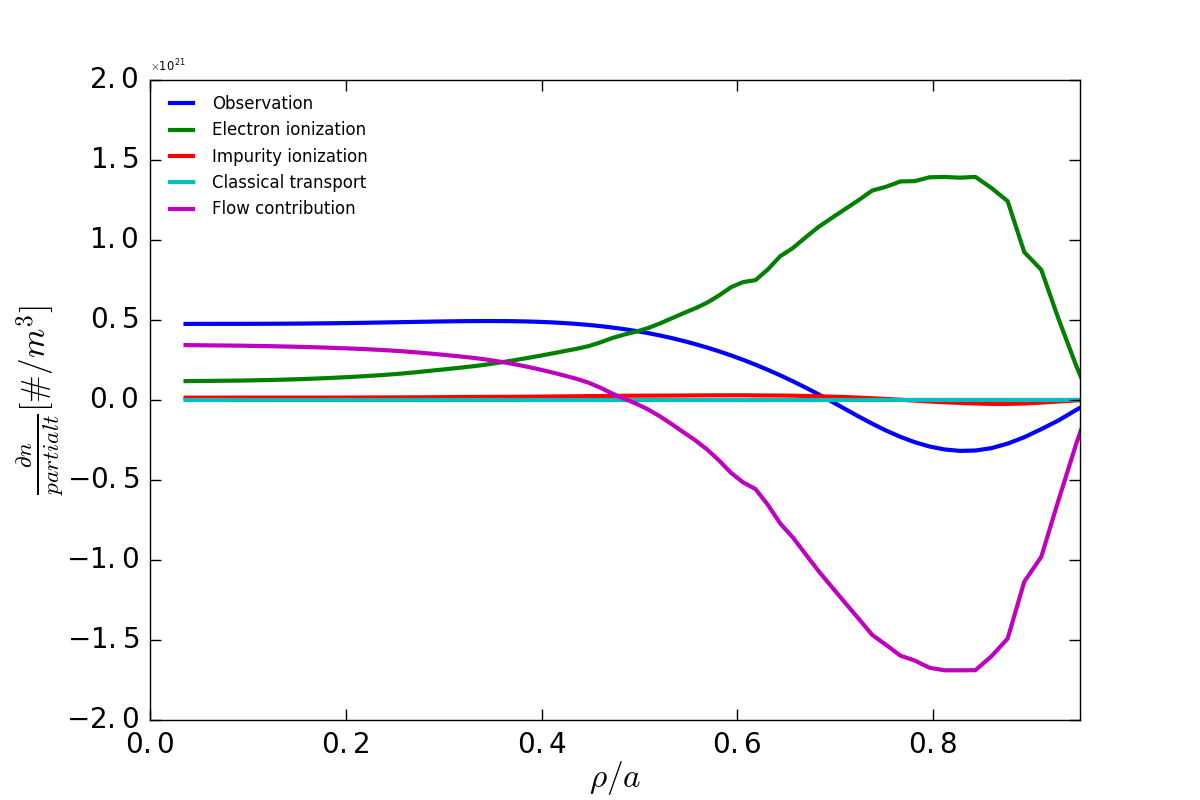
\includegraphics{ion_transport_results/density_balance.png}
    \caption{$\partialt n_e$ in MST and their sources. This particular plot presents the ensembled analysis at 14ms.}
    \label{fig:density_balance}
    %%TODO, need larger legend text.
\end{figure}

The first step is realizing that source rate mechanisms are limited. Ionization of deuterium and impurities accounts for all the available sources of electrons. However, particle flow has not been explored to the same degree. In J. Reynolds's thesis on simulating the effect of PPCD using the numerical MHD code NIMROD \cite{Reynolds2007}, he observes the simulation undergoing an inward pinch flow across the simulated plasma volume (see figure \ref{fig:NIMROD_pinch}). He also refers to previous simulation studies on PPCD-like conditions showing inward pinch\cite{StuffThatReynoldCited}. More empirical on MST, PPCD drive the plasma into deep reversal and the reversal surface moves inwards during this process. Previous measurements of electron density using FIR also show the gradient region moving inwards (figure \ref{fig:Ne_gradient_pinch}), hinting at a pinch. After all, it is in the name of the configuration.

\begin{figure}
    \centering
    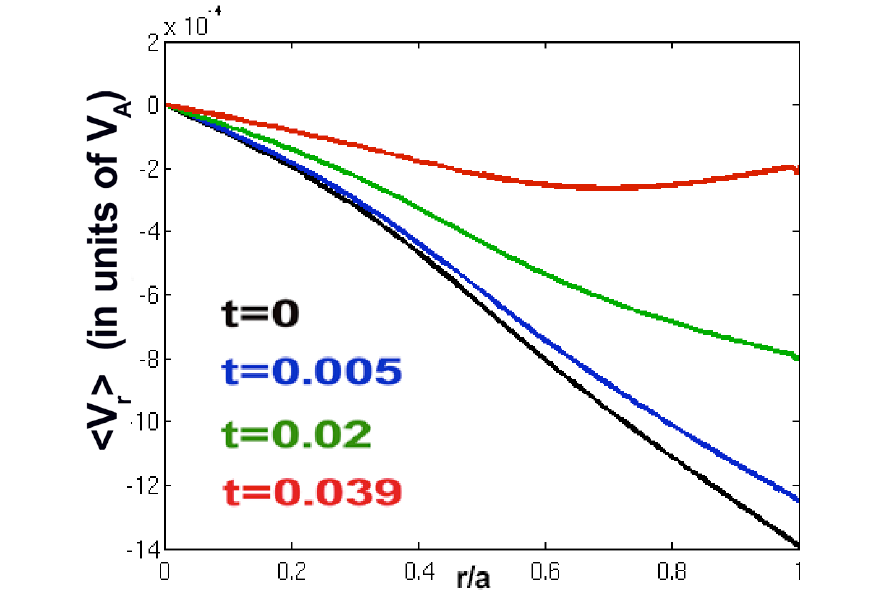
\includegraphics{ion_transport_results/reynold_pinch.png}
    \caption{Pinch velocity from J. Reynolds' simulations. Note that the simulation volume ends at the reversal surface and the Lunquist number of the simulation is lower than actual plasma conditions. (Reproduced from J. Reynolds\cite{ReynoldsThesis}). }
    \label{fig:NIMROD_pinch}
\end{figure}


Working with the hypothesis that the unaccounted for core density rise is due to a pinch flow, I use the continuity equation (equation \ref{eqn:continuity}) to calculate the particle flux needed to balance out the observations. This forms a basis for comparison with the hypothesized mechanism, \ecb drift.

\subsection{Estimating radial \ecb drift}

MST have limited ability to diagnose $\vec{E}$ field in high current plasmas. Thus the $\vec{E}$ needs to be estimated from indirectly from the $\partialt\vec{B}$ according to the Maxwell equations. The $\vec{B}$ field are calculated by the equilibrium reconstruction code MSTfit using inputs from the gap voltage measurements, edge pick up coils, and FIR polarimeter measurements. Sequential MSTfit equilibrium reconstruction are used to estimated $\partialt\vec{B}$. From there $E_{pol}$ can be calculated through:
\begin{align}
   E_{pol}(\rho_v) & = -\frac{1}{\rho_v}\int_{0}^{\rho_v}\rho_v' \frac{dB_{tor}}{dt} d\rho_v'
\end{align}
where it is taken as a boundary condition that the $E_{pol}$ is zero at the magnetic axis.

The calculation of $E_{tor}$ is slightly more complicated, as it is a function of major radius and not $\rho_v$. The voltage measurement ($V_{PG}$) across the poloidal gap on MST (a cut in the vacuum vessel along its intersection with the poloidal plane) is a reflection of the toriodal E field at the wall and serves as the boundary condition for the integration. $E_{tor}(R, Z=0)$ along the Z = 0 plane is determined as a function of major radius (R) through:
\begin{align}
\oint_S \vec{E}\cdot d\vec{l} &= -\iint \frac{\partial}{\partial t}\vec{B}\cdot d\vec{s}\\
E_{tor}(R) 2\pi R &= -\int_0^{2\pi}\int_{R_{in}}^{R}R'\frac{\partial B_{pol}}{\partial t} d\phi'dR' - V_{PG}\\
E_{tor}(R) &= -\frac{1}{R}\int_{R_{in}}^{R}R'\frac{\partial B_{pol}}{\partial t} dR' - \frac{V_{PG}}{2\pi R}\label{eqn:E_tor}
\end{align}
where $R$ refers to the major radius, and $R_{in}$ is the major radius at the inboard wall. To incorporate into the 1-D approximation, the inboard and outboard $E_{tor}$ is averaged according to their flux surface subsequently. From these, we can calculate the radial \ecb flux,
\begin{align}
    \Gamma_{\vec{E} \times \vec{B}} &= n_e v_{\mecb} \nonumber \\
    &= n_{e} \frac{E_{pol}B_{tor} - E_{tor}B_{pol}}{B^2}
\end{align}
The result of this calculation is shown in figure \ref{fig:eb_v}. This can be compared with the observed flux calculated from the continuity equation (figure \ref{fig:eb_v}). The result show that \ecb is a good explanation for the inwards flow needed to balance out the observations. Hence, the $\partialt n_e$ rise in the core can now be accounted for in such a way that the associated ion temperature is no longer arbitrary, since \ecb flow is ambipolar.

\begin{figure}
    \centering
    \includegraphics{ion_transport_results/eb_v.png}
    \caption[Calculated \ecb pinch velocity]{Calculated \ecb pinch velocity. The velocity is plotted to the reversal surface. Compares well with MHD simulations results in figure \ref{fig:NIMROD_pinch} qualitatively. }
    \label{fig:eb_v}
\end{figure}
\begin{figure}
    \centering
    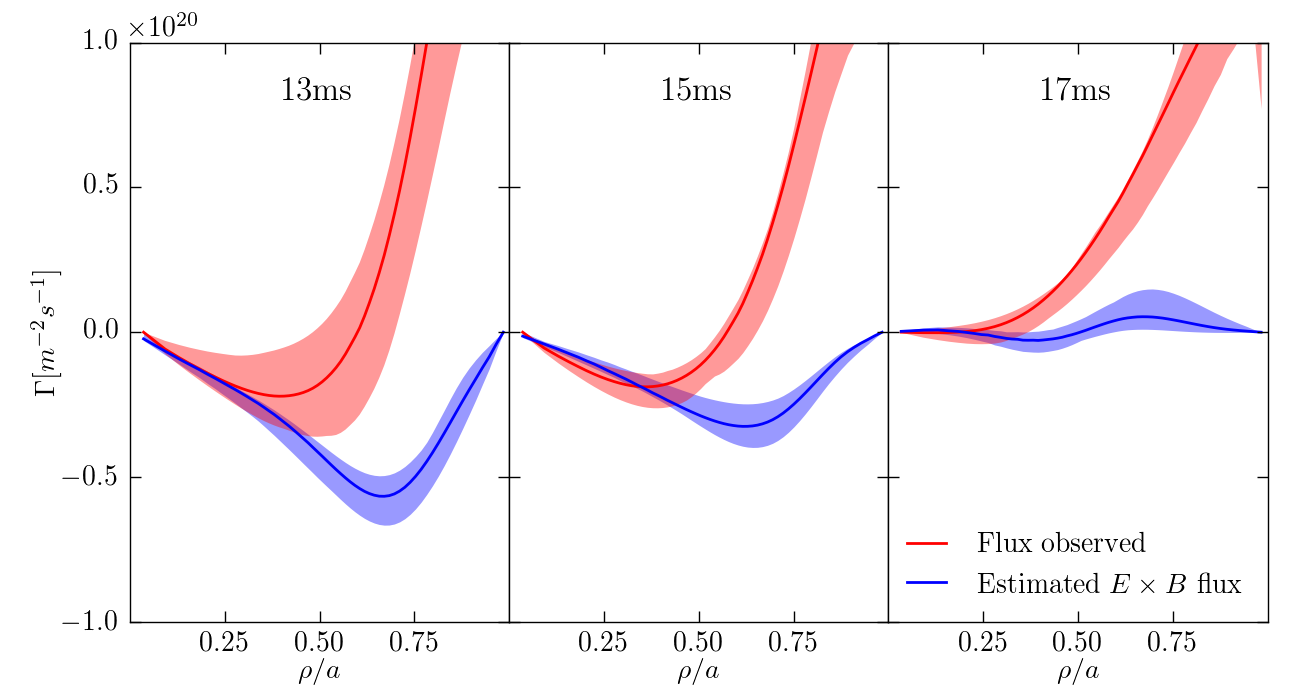
\includegraphics{ion_transport_results/flux_comp.png}
    \caption[\ecb flux compared to measured flux]{\ecb flux compared to the observed flux. 'Observed' flux is that implied by the continuity equation though $\partialt n$ and source rate observations. The two match until the mid-radius. The outer areas of the plasma is dominated by an outward anomalous particle flux. The outward flux at the edge is consistent with previous estimates\cite{TakashisSource}. }
    \label{fig:eb_v}
\end{figure}

\subsection{Flow effects on thermal transport}

The effects of the flow can be calculated via the method laid out in section \ref{sec:flow_effects}. It is useful reiterate the two components of the flow effect. One has to do with the conservation of the energy being carried by the ions. This term brings energy into the core, but generally will result in cooling, whereas it brings energy out of the edge (loss to wall), but is general increasing temperature as they are 'replaced' by ions flowing out from mid-radius. The other term is the compressional work by the \ecb drift in varying fields. This is calculated from the estimated drift velocity, and is a mostly positive term, and since it doesn't not have density effects, it represents a temperature increase. The details of these two terms are presented in figure \ref{fig:flow_power_terms}. 

\begin{figure}
    \centering
    \includegraphics{ion_transport_results/flow_power_terms.png}
    \caption[Power terms resulting from radial ion flow]{Power terms resulting from radial ion flow.}
    \label{fig:flow_power_terms}
\end{figure}

\section{Model comparison with measurements: anomalous heating in the edge.}\label{sec:results_results}
\begin{figure}
    \centering
    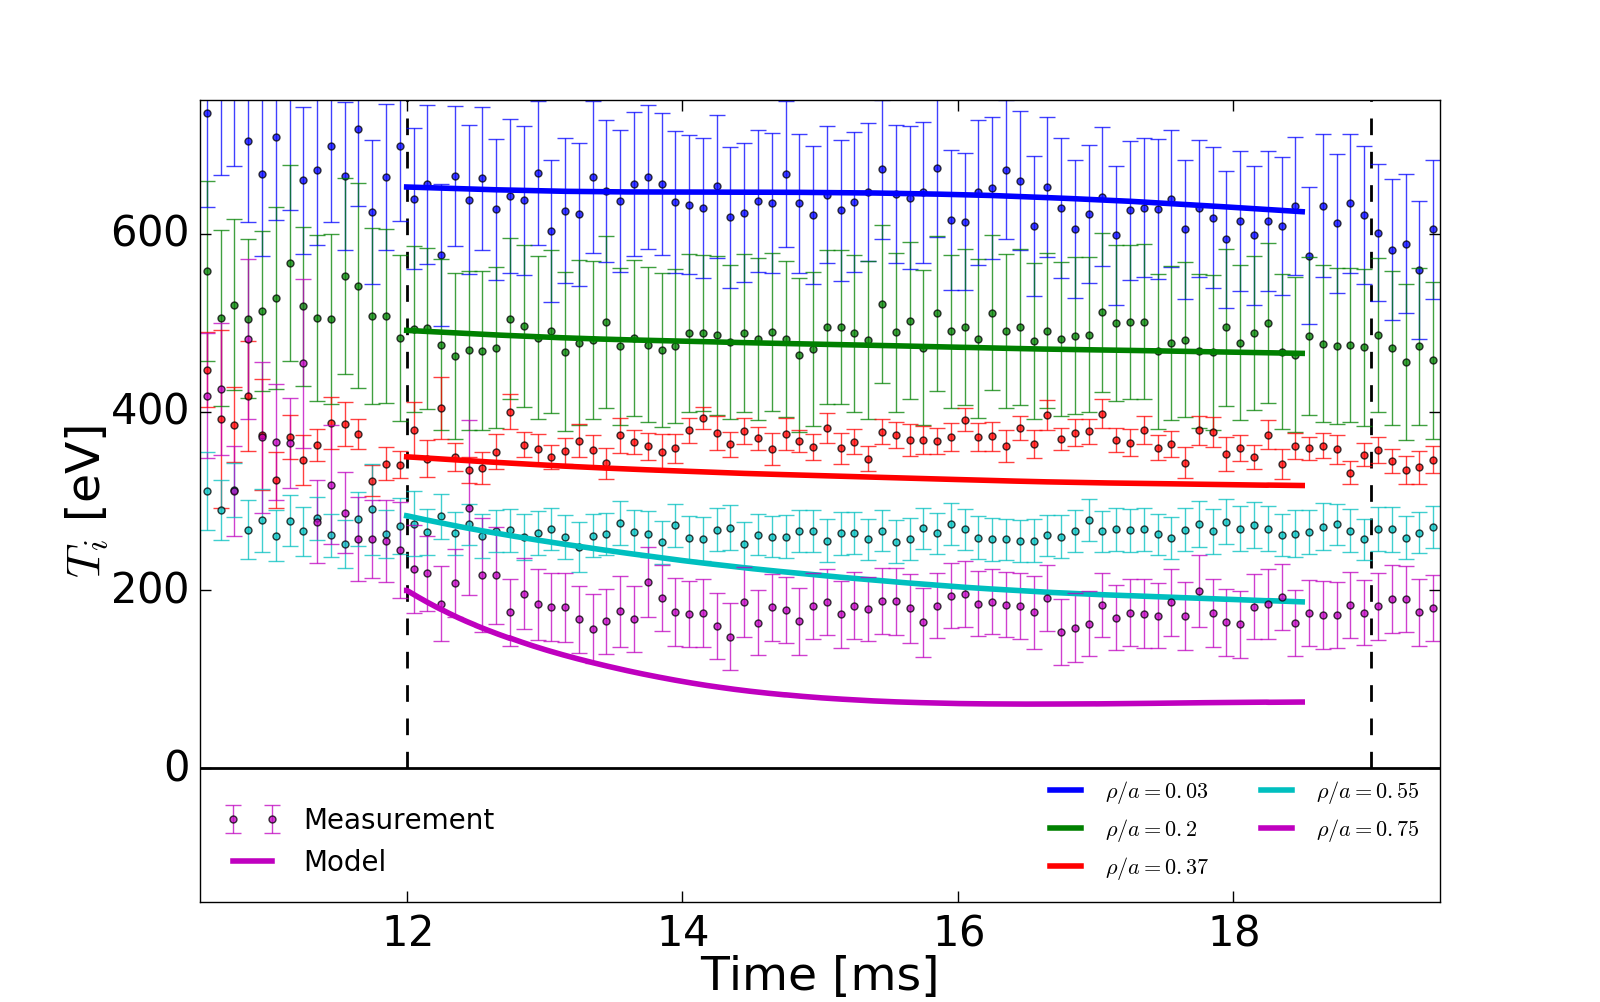
\includegraphics[width = \linewidth]{ion_transport_results/temperature_results.png}
    \caption[Temperature comparison with measurement]{Temperature comparison with measurement.}
    \label{fig:temperature_results}
\end{figure}

\begin{figure}
    \centering
    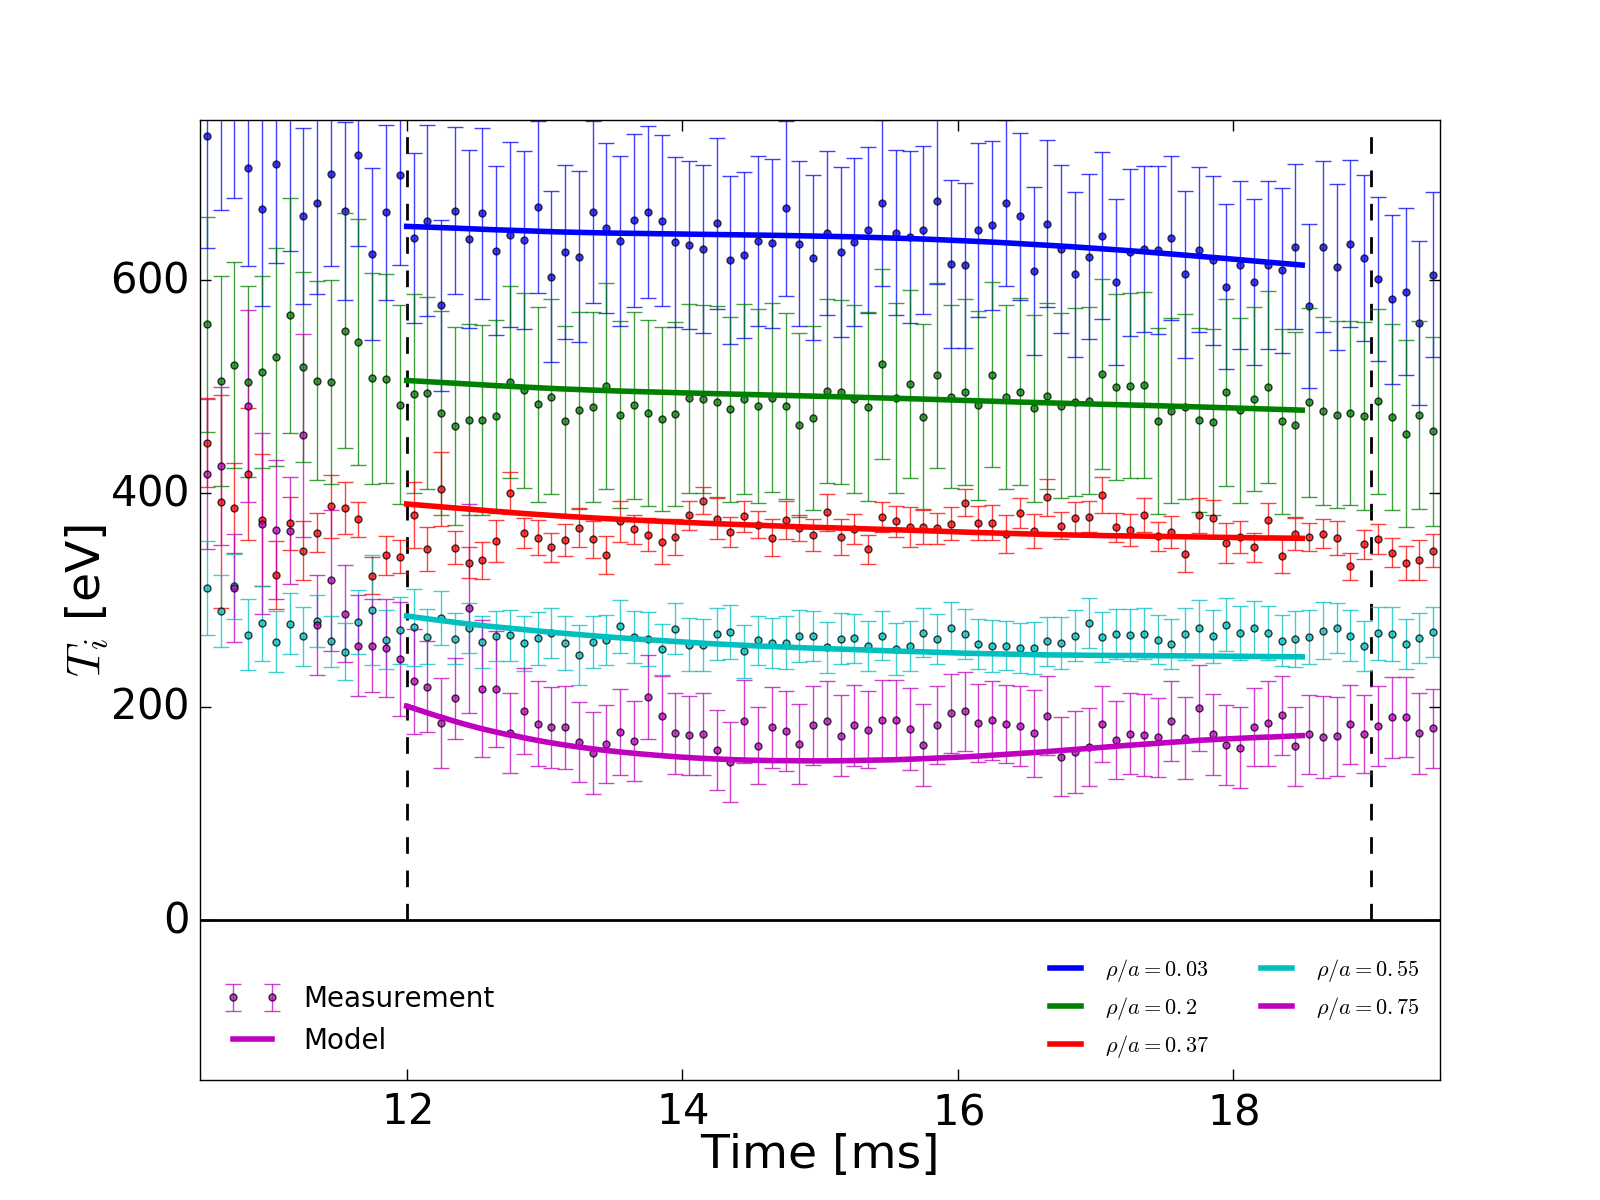
\includegraphics[width = \linewidth]{ion_transport_results/temperature_with_adhoc.png}
    \caption[Temperature comparison with measurement with \textit{ad hoc} term included]{Temperature comparison with measurement with \textit{ad hoc} term included.}
    \label{fig:temperature_results_ah}
\end{figure}

\begin{figure}
    \centering
    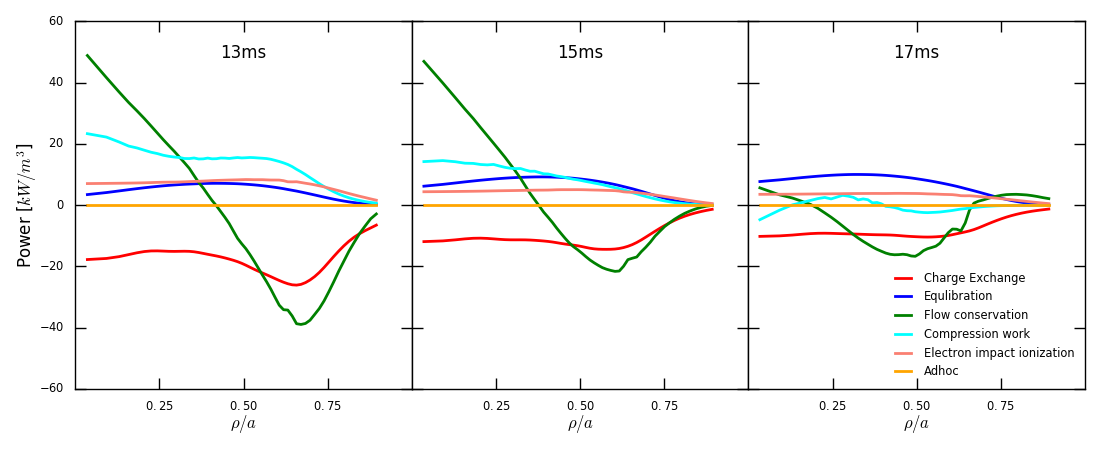
\includegraphics[width = \textwidth]{ion_transport_results/power_terms_no_adhoc.png}
    \caption[Power terms resulting from radial ion flow]{Power terms resulting from radial ion flow.}
    \label{fig:power_terms_no_ahoc}
\end{figure}
The quality of the model is evaluated by comparing its prediction to the ion temperature measurement made with CHERS. The model is initiated at 12ms, about 2ms after the first PPCD capacitor bank 'fires', as it is the earliest time when the significant suppression of tearing mode turbulence are achieved. CHERS measurement of temperature at initialization time is fit to an alpha model profile and then input into the model as initial condition. The time evolution of ion temperature is calculated according to the physics terms described in the previous sections and chapters. The model is found to adequately predict the temperature in the core, but not in the edge. To account for the edge temperature, an \textit{ad hoc} heating term is added. The model comparison results can been seen in figure \ref{fig:temperature_results}.  The most significant power loss terms (figure \ref{fig:power_terms_no_ahoc}) affecting this region is charge exchange, and thermal energy carried by particle flow (flow conservation). It is interesting to note that these loss terms are to a large extent a function of temperature as much if not more than as a function of temperature gradient. This dependence on $T_i$ is a factor that result in there being an 'equilibrium' temperature for the model. For the case where no \textit{ad hoc} heating is included, the ion temperature at near the edge would decrease until it levels off at significantly lower temperatures than the measured. In particular, figure \ref{fig:temperature_results} superficially suggest that (for the edge chord location) the temperature decreases rapidly early during the PPCD period. But initializing the model at later starting time would have the model reproduce the same behavior and settle at the same edge temperature, just now delayed. This indicates that it is not some particular circumstance relating to the early PPCD period that causes the model to under predict the temperature. But the model behaves in such a way that the edge temperature trends towards and `equilibrium' temperature determined by the power terms, which is significantly lower than the actual equilibrium temperature that the ion fluid comes to. To remedy this under prediction, an \textit{ad hoc} term is introduced into the model to raise the model's 'equilibrium'. The particular profile shape and location used for the \textit{ad hoc} term is discussed in detail in the next section, but the result of this are presented in figure \ref{fig:temperature_results} and \ref{fig:power_terms_with_adhoc}. With this addition, the model is able to account for the temperatures measured by CHERS. In this scenario, the core power terms are dominated by the effects of flow, in particular compressional heating and flow conservation. It is also useful to refer to figure \ref{fig:temperature_change} which provides information on how each term effects $T_i$. From this figure it is easier to see the importance of the compressional heating term on the core temperature prediction. $P_{\text{comp work}}$ is the larger of only two terms increasing temperature in the core, and is a major part of how the model matches a flat-ish fore $T_i$ evolution observed. Towards the edge, the major heating (thermal energy input) term is the \text{ad hoc} term. $P_{\text{flow cons}}$ is negative in the edge and the most significant source of loss. One looking at $\partialt T_i$ plot would come to the (almost) paradoxical conclusion the the flow conservation term is significant in maintaining temperature. This can be understood by pointing out the outward particle flow in the edge have the net effect of removing a number of ions at the local temperature, and replacing them with a smaller number of hotter ions from inner flux surfaces, thus increasing temperature. The density balance is achieved though a large ionization source rate, which reduces $T_i$ despite bringing some thermal energy with it (due to non-zero neutral temperature).


\begin{figure}
    \centering
    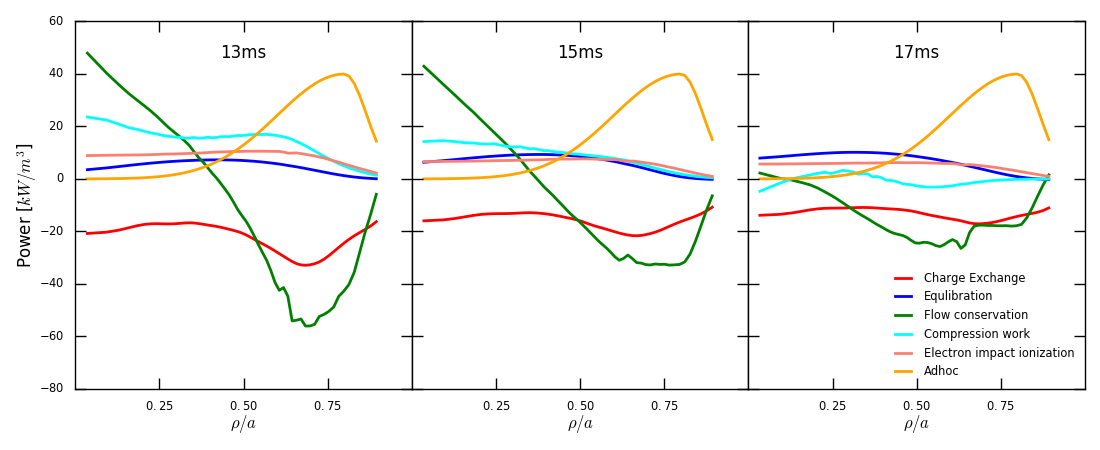
\includegraphics[width = \textwidth]{ion_transport_results/power_terms_with_adhoc.png}
    \caption[Power terms resulting from radial ion flow]{Power terms resulting from radial ion flow. Classical conduction have been omitted as it is of lower magnitudes than the plotted terms.}
    \label{fig:power_terms_with_adhoc}
\end{figure}


%TODO: There should be a paragraph on estimating the ion thermal confinement time that I'm not quite ready to write yet. 

From this model, the ion thermal confinement time can be estimated. The common definition of thermal confinement time is written as follows,
\begin{align}
    \tau_E &= \frac{W}{P_{\text{loss}}}\\
    &= \frac{W}{\partialt W - P_{\text{ohm}}}
\end{align}
However, in the context of the model, where the loss terms are known explicitly, it is more appropriate to specify $P_{\text{loss}}$ directly. In particular, 
\begin{align}
    P_{\text{loss}} &= - [P_{\text{CX}} + P_{\text{cond}} + P_{\text{flow cons}}]
\end{align}
The other terms in the model, including compressional work, \adhoc heating, and e-i equilibration heating, are considered power inputs, and thus do not factor into the calculation of the thermal confinement time. 
 % I don't think that these terms are 'external' to the plasma the way Ohmic heating or RF heating are external inputs to the plasma. By they are power inputs to the ion fluid rather than losses.
 %Edited -Xing
This means that for the consideration of this calculation, the flow terms as specified in section \ref{sec:flow_effects} are separated into the compressional heating part ($P_{\text{comp work}}$) which is not part of $P_{\text{loss}}$, and the flow conservation part ($P_{\text{flow cons}}$) which is. The confinement time of the model is shown in figure \ref{fig:conf_time}. It should be noted that this is not a direct measurement of the ion confinement time, but rather it is the ion confinement of a model that can be matched to observed temperature evolution.
\begin{figure}
    \centering
    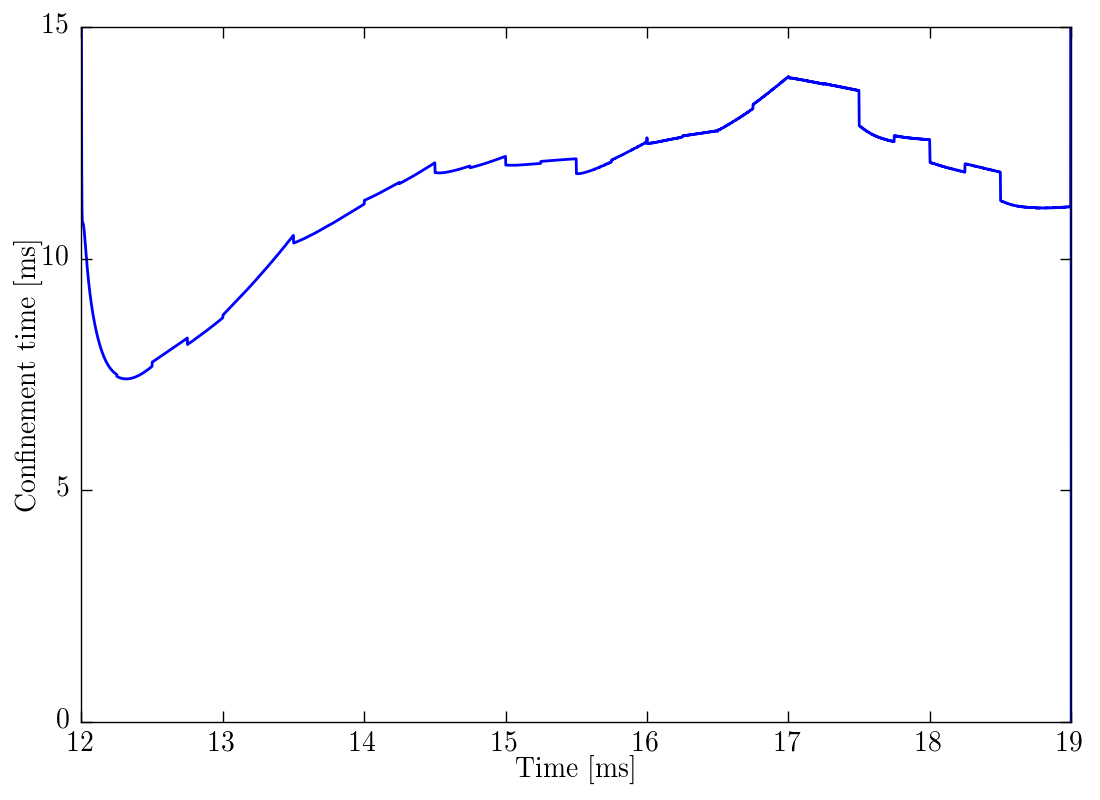
\includegraphics[width = \linewidth]{ion_transport_results/conf_time.png}
    \caption[Model ion confinement time]{Ion confinement of the model. It is calculated to be around 12ms for the 'main' part of PPCD (~15ms to the end of PPCD). The confinement time is poorer during onset of PPCD (< 15ms) but displays a roughly upward trend. The effect on temperature of this relatively poorer confinement is mitigated by the compressional heating active during the early period. }
    \label{fig:conf_time}
\end{figure}
The thermal confinement time is comparable to electron confinement time in PPCD calculated at ~ 10ms \cite{Chapman2001}, but it is not evident that the two are linked through physical mechanisms. Considering the decoupling of ion and electron temperature, it may be a coincidence that their confinement time seems to match. The model's confinement time further changes if the model temperatures are allowed to drift below the observed temperature by omitting the \adhoc heating term. In that case, the confinement time noticeably increase as the edge ion temperature decreases which decreases the heat loss due to outward particle flux in the edge, as well as somewhat reducing the charge exchange loss the the same region. 
%%% Now that you have calculated the ion thermal confinement time, how does it compare with other relevant time scales? For instance, how does it compare with the electron thermal confinement time for PPCD or standard plasmas? Are the results what you would expect or are they surprising?
%Elaborated. --Xing

\subsection{Profile and extent of \adhoc heating in the gradient regions}\label{sec:anomalous_heating}

The previous section glossed over the shape and location of the \textit{ad hoc} heating term used in order to present the results. However, there are comments to be made that would be of interest to readers. The driving determinant of the \textit{ad hoc} term is to enable the model to match the observations, but that does not mean that it is entirely free of physics considerations. The profile settled upon is an asymmetrical Gaussian (in $\rho_v$) made from two half Gaussian profiles with differing width. The profile peaks at $\rho_v/a = 0.75$, the approximate location of the reversal surface (see figure \ref{fig:q_profile}). The reversal surface is not only the home of all m = 0 modes, but also near tightly packed m =1 rational surfaces. Additionally, the peak and the width of the \textit{ad hoc} heating term is approximately coincident with the $T_e$ gradient region as measured via Thomson scattering. The edge half of the Gaussian shape have a smaller width to account for the fact that the turbulence that likely drives anomalous heating would be rapidly decreasing near MST's conducting shell, together with rapidly decreasing availability of free energy as temperature and density drops in the very edge. However, the modeling work and the CHERS measurements provide nearly no constraint on the very edge of the plasma. 
\begin{figure}
    \centering
    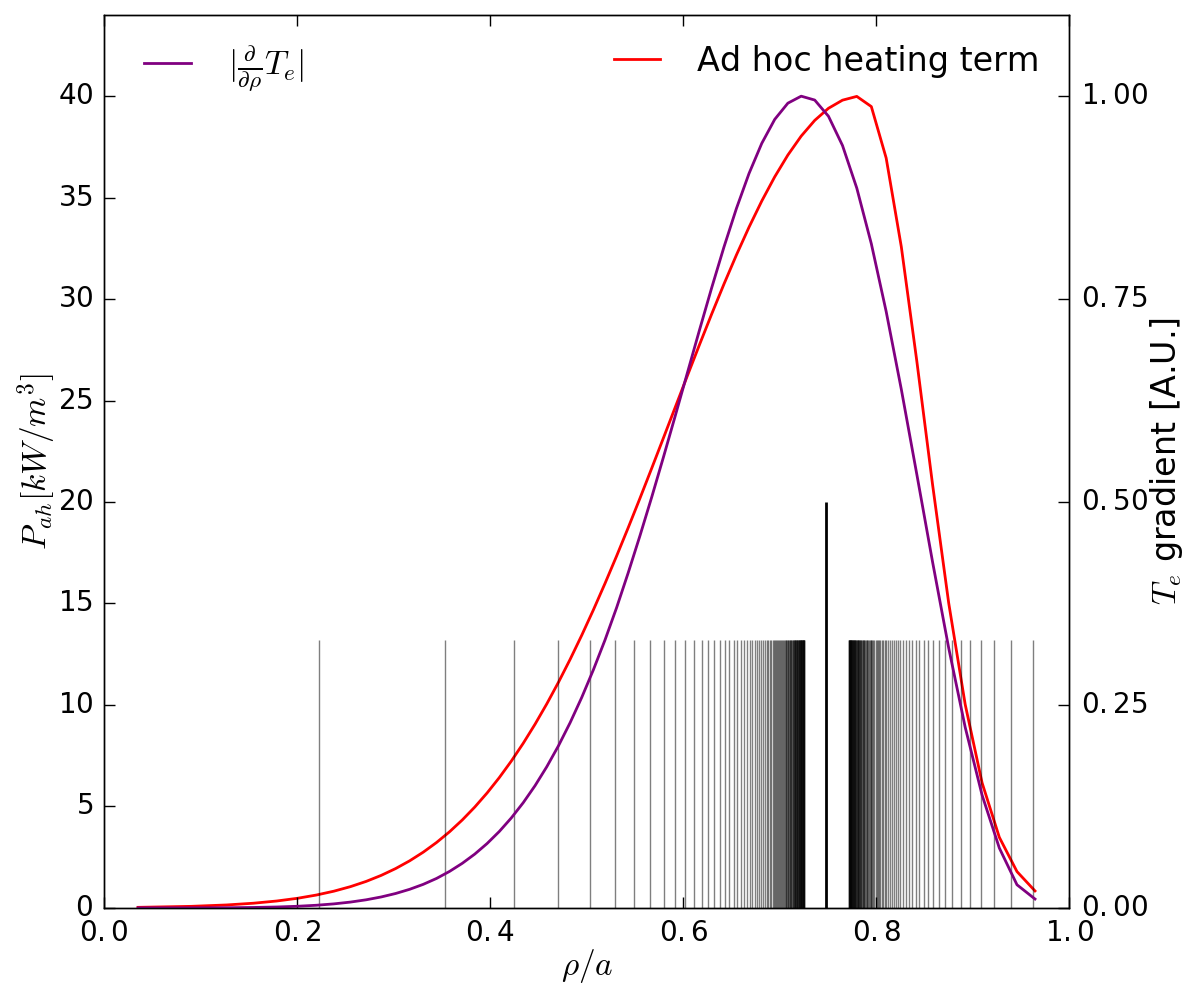
\includegraphics[width = \textwidth]{ion_transport_results/adhoc_profile.png}
    \caption[\textit{ad hoc} heating profile]{\textit{ad hoc} heating profile compared to normalized $T_e$  gradient. The long vertical line at $\rho/a \approx 0.75$ marks the location of the reversal surface, and the shorter lines marks out the resonant surfaces beginning with inner most the (1,6) surface. For a plot of the q profile associated, see figure \ref{fig:q_profile}.}
    \label{fig:ad_hoc_v_gradient}
\end{figure}
%Mark comments here:
%In addition to mentioning the edge localization, you should note that there are several sources of free energy that could drive heating mechanisms. First, there is residual tearing mode activity in PPCD plasmas that, while much lower in amplitude, still result in stochasticization of the magnetic field near the reversal surface. In addition, we are actively driving a current in the edge and may be affecting the current gradient in such a way that it can excite the edge-resonant modes. Finally, there is the edge density gradient which drives drift wave instabilities that give rise to turbulent electrostatic fluctuations.

%These are all free sources of energy that could provide sufficient energy for the modest amount of edge-localized ion heating your model suggests. This energy could be tapped through processes like turbulent damping of Alfven-waves through cyclotron resonance, stochastic heating due to the residual tearing modes near the reversal surface, driving edge-resonant tearing through the PPCD pulses, and turbulent heating which can channel heat from the electrons to the ions.
 
%For the last process, I started with Gennady’s paper and potentially made a mistake. For Gennady’s argument to be self-consistent the perpendicular diffusion process has to be separate from the process generating the electric field fluctuations. Otherwise, there is a problem with making the process irreversible.

%A more natural way of formulating the heating mechanisms available through drift wave turbulence is to consider ion Landau damping and frictional heating associated with zonal flow generation by the turbulence. A paper which lays these mechanisms out is here:
There are several mechanisms that may be responsible for this \adhoc heating, including cyclotron resonance heating from Alfven waves and stochastic heating from residual tearing modes activities near the reversal surface. Further, plasma turbulence such as driftwaves and zonal flow, both recently observed for PPCDs in MST\cite{Nishizawa2018, Nishizawa2019}, drives both quisilinear and nonlinear turbulent heating and enables the collisionless transfer of energy from electrons to ions through such mechanisms such as Landau damping of wave energy, and frictional heating via zonal flow. The volume integrated \adhoc heating used in the model is $\approx 144 kW$, which is small in the overall energy balance of the RFP. For example, the total magnetic energy ($ = \frac{B^2}{2\mu_0}$) goes from $\approx 275kJ$ to $\approx 300kJ$ and back during a typical period of analysis (spans 8ms from 12ms to 20ms). Thus a seemingly small transfer of energy from electrons or the magnetic equilibrium may be sufficient to account for the \adhoc heating added to model calculations.

More generally, the location and the width of the \textit{ad hoc} heating term roughly corresponds with the location of the $T_e$ gradient region (see figure \ref{fig:ad_hoc_v_gradient}). While electron gradients are not directly connected to ion thermal heating, they are sources of free energy driving turbulence that would generate heating. 

\subsection{Anomalous Transport vs. heating}

The \textit{ad hoc} heating term needed for the model can correspond to anomalous transport or heating, as the model does not account for stochastic transport mechanisms, or turbulent heating mechanisms. However, given the model's ability to predict the core temperature well even in the absence of the \textit{ad hoc} term, it is more likely that the discrepancy in the edge is accounted for by anomalous heating. 
Consider stochastic transport of heat, the stochastic counterpart to classical thermal conduction. The stochasticity increases the characteristic step size of the particle beyond the gyro-radius, and ions wondering along the stochastic field would collide another and exchange place' with it, transporting heat from the hotter location to the colder. Note that this is a purpose effort to separate the stochastic heat conduction/transport from the stochastic particle transport, as the particle transport and flux is indirectly included in the model (see the discussion in section \ref{sec:stochastic_effects}). The total \adhoc term needed in the model integrates to about 140kW over the volume of the plasma. If the \adhoc term is 'caused' by a anomalous transport mechanism, then the transport mechanism would be taking the thermal energy from hotter regions (\textit{ie.} core). For an estimation, one can assume that such a transport mechanism takes heat from the core region defined by $\rho/a \leq 0.4$ and deposit at $0.4 \leq \rho/a \leq 0.9$ (refer to figure \ref{fig:ad_hoc_v_gradient}). Thus defined, the core region have a volume of $\approx 1.25 m^2$, and lose heat at $~110kW/m^2$ making it the most significant term in the core. Further assuming a nominal core density of $0.7 \times 10^{19}/m^3$, the core cooling implied by such a transport would be $\approx 100eV/ms$ in addition to what the model currently predicts. This is significantly larger core cooling than the observations would allow (refer to figure \ref{fig:temperature_results_ah}).

While it cannot be ruled out that the \adhoc term in the model is the result of a combination of a anomalous transport mechanism, and a (relatively) radially uniform anomalous heating mechanism, it is very unlikely to be the effect of a anomalous transport mechanism only. To the first order, the result point to an anomalous heating mechanism active in the $T_e$ gradient region.

\subsection{Additional comments on thermal transport}

\begin{figure}
    \centering
    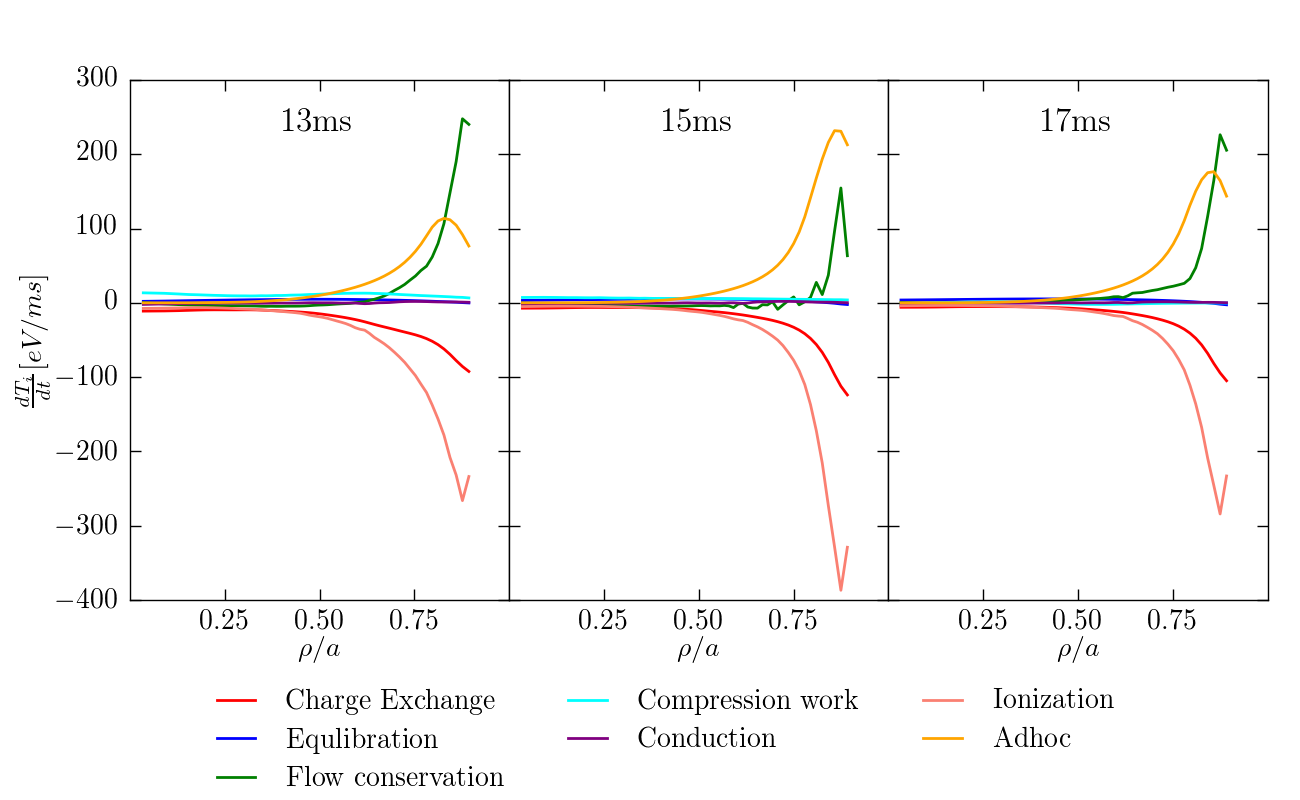
\includegraphics[width = \linewidth]{ion_transport_results/dtempdt_with_adhoc.png}
    \caption[$\partialt T_i$ due to various terms]{$\partialt T_i$ due to various terms in the model. The significance of this plot is explored more in the text. }
    \label{fig:temperature_change}
\end{figure}

\begin{figure}
    \centering
    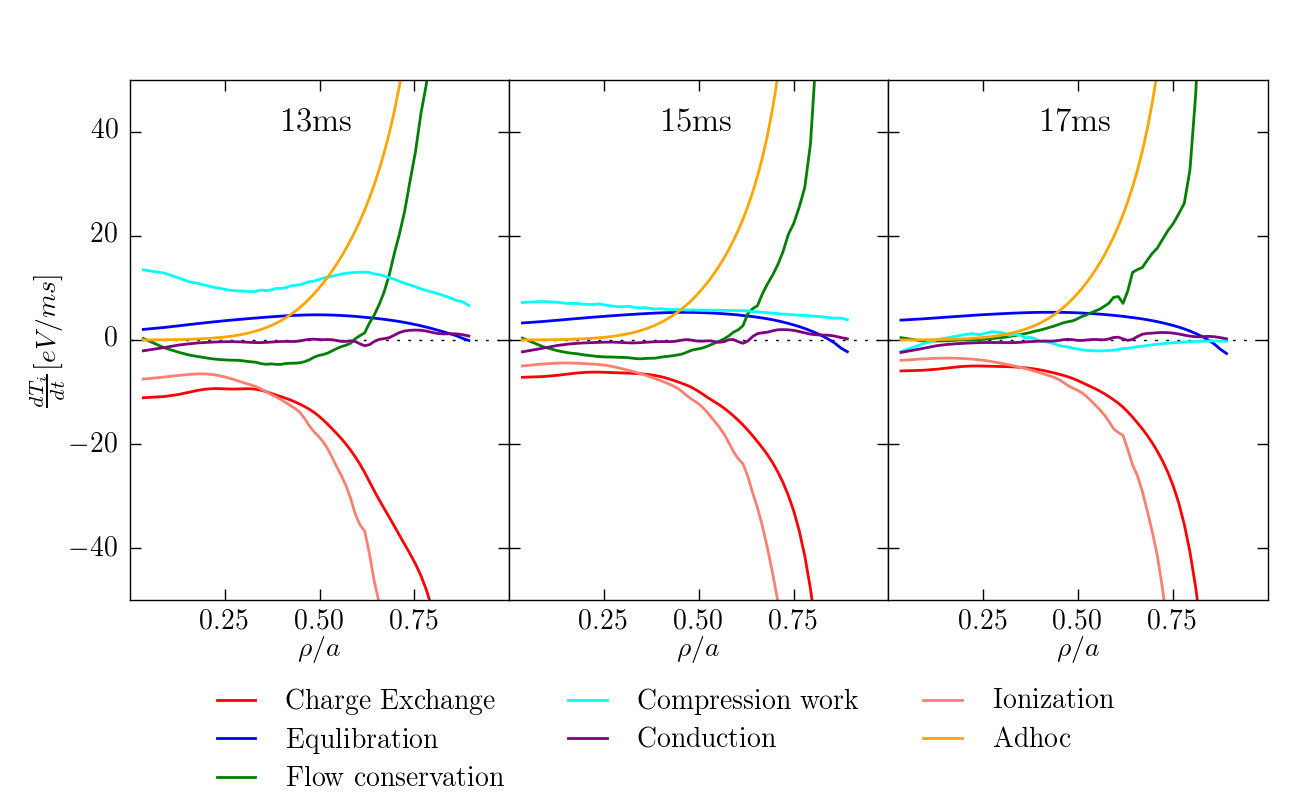
\includegraphics[width = \linewidth]{ion_transport_results/dtempdt_zoomed.png}
    \caption[$\partialt T_i$ core details]{$\partialt T_i$ due to various terms in the model, zoomed in to show the core dynamics clearer. Note the disappearing effect of compressional work. }
    \label{fig:temperature_change_zoomed}
\end{figure}

It is instructive to look at the modeled terms from the point of view of their contribution to $\partial T_i /\partial t$ (figure \ref{fig:temperature_change} and figure \ref{fig:temperature_change_zoomed}). There is two effects worth noting. The first is that some power terms do not have the same effect on temperature as thermal energy. As mentioned before, $P_{\textrm{ionization}}$ which represents the energy 'recovered' from the warm neutral population through re-ionization, reduces the ion temperature despite being a positive power term. This is due to the fact that it brings cooler particles into to the ion fluid. The cooling effect of ionization is the most significant in the edge region, but important throughout the plasma volume. Conversely, the flow effects are (aside from the \textit{ad hoc} term) the most significant for increasing the temperature, due to the flow of hotter ions to the cooler edge. But at the same time, it competes with charge exchange for being the significant energy loss term. The second is that the $P_{\textit{ad hoc}}$ contribution to $\partial T_i / \partial t$ is modified by density, causing it to chage despite the power remaining constant. Especially, it's peak is farther out in the edge as compared to that of $P_{\textit{ad hoc}}$ itself. Looking at figure \ref{fig:temperature_change_zoomed}, we can see that \textit{ad hoc} term's contribution to $\partial T/\partial t$ is relatively constant inside $\rho/a = 0.75$. The response outside of this location (\textit{i.e.} the outside half-Gaussian of the \textit{ad hoc} profile) changes significantly. Though the model is not well constrained here, as the outer most CHERS measurement is at $\rho/a = 0.75$. If the \textit{ad hoc} heating is indeed related to the stochastic mechanism as detailed by G. Fiksel, the $\left.\partial T_{i}/\partial t\right|_{\textit{ad hoc}}$ would be relatively constant and the resultant power would change as density changed. 

The e-i equilibration term is generally weak, resulting in the temperature separation seen in PPCD plasmas. Extrapolating to typical reactor densities, however, would imply that the equilibration heating would in crease by ~ 2 order of magnitude (both $n_e$ and $n_i$ would increase by an order of magnitude) while the biggest core loss term, charge exchange, would increase less as the neutral sourcing will increase will plasma density, but the neutral penetration will decrease correspondingly. As is currently, the charge exchange loss and the net flow loss (aka particle loss) are the two main loss mechanisms. Efforts to limit neutrals in the plasma may be beneficial, but high density and temperature plasmas, the neutrals are likely to have a much reduced role. Net ion particle loss will likely be the dominant challenge to RFP ion confinement in PPCD-like conditions. 



\section{Summary}

Experimental results show the 1-D ion thermal transport model adequately predicts the ion temperature evolution in the core, but needs an \adhoc term in the gradient region to match observations there. Of particular importance to the model is the neutral dynamics as calculated via the Monte-Carlo simulation code DEGAS2. This simulation is important in calculating the charge exchange loss from the core. The results indicates that the neutral population in the core is 'warm' and the charge exchange loss is somewhat hollow. The ionization of neutrals are found to 'recover' some of the energy lost to the neutral fluid, but this results in decrease in temperature. The source rate geometry and continuity equations calculations finds that PPCD plasmas under goes an inward pinch during the first milliseconds, which contributes to core temperature via compression. However, the net particle flux at the edge is outwards and represents a significant loss term. When compared to ion temperature measurements, the model is found to be unable to match the observation in the gradient region unless an radially local \adhoc heating term is added. Comparisons are drawn between the \adhoc term needed and estimates of fluctuation induced heating and found to be plausible.


\printbibliography
\end{refsection}
\begin{refsection}

\chapter{Edge impurity ion heating associated with $m = 0$ activity in PPCD}\label{ch:m0}

In addition to the slower time scale ion thermal transport modeling, the particular phenomenon of impurity ion heating in connection with $m = 0$ bursts deserves some attention. Ideally, the m = 0 burst would not occur, and the datasets underlying the previous chapter are selected to avoid "bursty" PPCD shots. However, these $m = 0$ bursts and their heating effects are relatively small perturbations, especially compared with sawteeth events, making them interesting to study. Since they are brief events and the plasma returns to the PPCD quasi-equilibrium quickly, their effects can be more comfortably discussed as perturbations on a (relatively) known state. This section will first go into a brief discussion of the current understanding of $m = 0$ bursts, their characteristics and their broader context in relation to PPCD plasmas. Then I discuss the measurements of impurity carbon heating observed in relation to theses bursts. Finally, I present the results of modeling attempts within the framework of the ion thermal transport model discussed in previous chapters.

\section{Characteristics of $m = 0$ burst activity}
What is now called the $m = 0$ bursts is also referred to as "small dynamo events", especially in work revolving around the thesis of B. Chapman \cite{Chapman1997}. Similar to sawtooth events, the $m = 0$ bursts generate toroidal flux and poloidal current. However, unlike the sawtooth events, they first appear in the edge resonant modes, in particular the $m = 0$ modes (hence it's current name). These $m = 0$ bursts are observed in sawtooth surpressed axis-symmetric plasmas such as PPCD plasmas or the spontaneously occurring Enhanced Confinement (EC) plasmas. Despite it's name, the $m = 0$ burst does excite the $m = 1$ tearing modes as well shortly after the $m = 0$ mode (see figure \ref{fig:m0_time}), merely reversing the order of excitation as compared to sawtooth events. Further, it is not clear that the $m = 0$ bursts can be said to be caused by the destabilization of $m = 0$ modes, or that the $m = 0$ mode are themselves preceded by other instabilities. It is previously found that the frequency of $m = 0$ bursts can be reduced by reversing $E_{\text{tor}}$ at the edge during the PPCD period, thereby help maintain $E_\parallel > 0$\cite{Chapman2001}. Interestingly, the $m = 0$ bursts that persist in occurring after this optimization has been made are largely concentrated in the earlier part of the PPCD period, before edge $E_{\text{tor}}$ reverses (figure \ref{fig:m0_shot_time}).

\begin{figure}
	\centering
	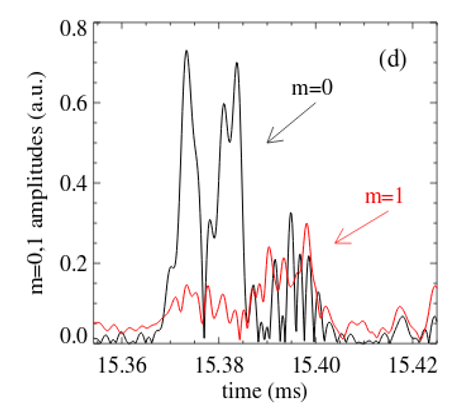
\includegraphics[width = .7\linewidth]{./m0_and_impurity_heating/m0_timing.png}
	\caption[$m = 0$ vs m =1 mode amplitudes during $m = 0$ burst]{$m = 0$ vs m =1 mode amplitudes during $m = 0$ burst (Reproduced from Piovesean\cite{Piovesan2008})}
	\label{fig:m0_time}
\end{figure}

\begin{figure}
	\centering
	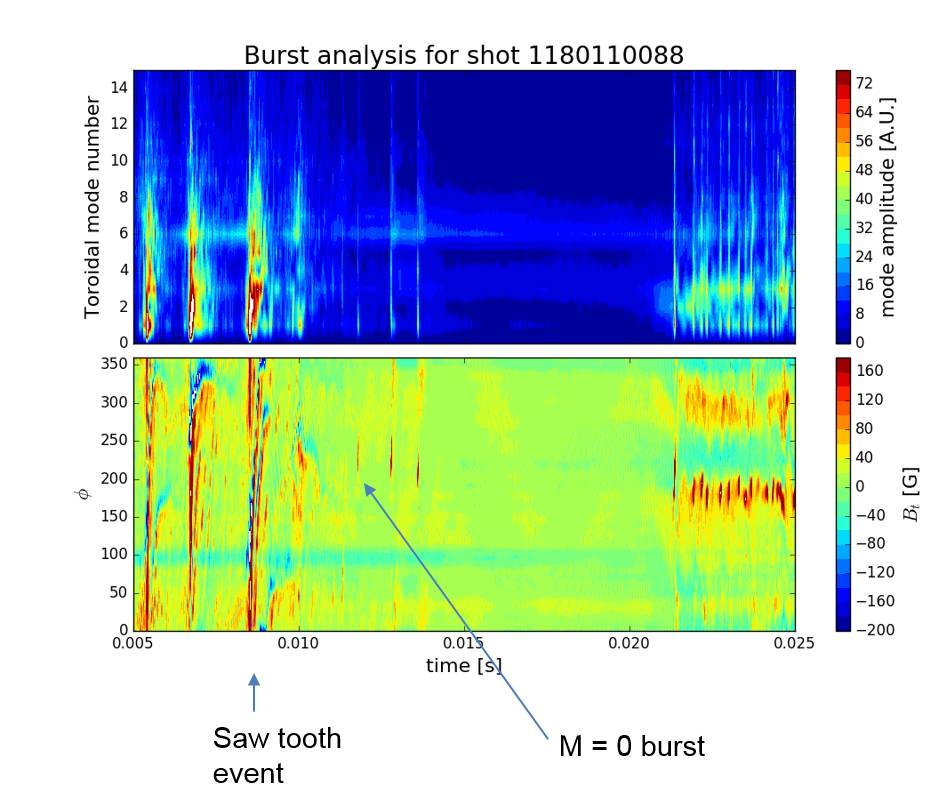
\includegraphics[width = 1.\linewidth]{./m0_and_impurity_heating/m0_example.png}
	\caption[Example mode and $B_t$ behavior]{Example of a typical bursty PPCD shot. The top presents a contour plot of the mode amplitudes vs time, broken down with respect to n number. On MST, m number break down is not always available but the $n < 6$ modes are $m = 0$ due to geometry constraints. The bottom presents a contour of the reconstructed $B_t$ values vs time and toroidal location ($\phi$). }
	\label{fig:m0_example}
\end{figure}

The $m = 0$ bursts involve a wide range of $n$ numbers with coherent phase in such a way that it reconstructs to a single larger perturbation at one particular location, akin to the relation between a Dirac delta and it's Fourier transform. A good way to visualize some aspects of the $m = 0$ burst is presented in figure \ref{fig:m0_example}. The top plot is the contour of the model amplitude vs. time and toroidal mode number ($n$), and on the bottom is a contour of the reconstructed $B_{\text{tor}}$ vs time and toroidal angle ($\phi$). The PPCD capacitor banks are engaged starting at 10ms, and the improved confinement achieved in this shot lasts until about 22ms, during which three $m = 0$ bursts are seen. In addition, three sawtooth events can also be seen at ~5.5, 6, and 8ms. The broad $n$ number excitation can be seen as well as the limited toroidal extent of the "main" perturbation. It can also be observed their relatively small amplitude and short duration as compared to sawtooth events. It is interesting to point out that the second burst seems to have energized the core ($n = 6$) mode, but the third burst de-energized it. It is generally the case that the bursts will generally interact with the core mode, but not in an easily generalizable way. Previous studies of $m = 0$ bursts conducted by Piovesean et al.\cite{Piovesan2008} find that the magnetic field measurements can be explained by a simple model, where a poloidal, field-aligned current filament that spontaneously arises, and travels in the toroidal direction for a short time before disappearing. In addition, a broad spectrum of $m = 1$, high $n$ fluctuations are also excited and propagate toroidally.  The effect of individual bursts on transport is small\cite{Piovesan2008}. In the high current PPCD studied in this work, the typical burst results in a $B_{\text{tor}}$ perturbation with toroidal width of $\approx 10\degree$ and travels $\approx 40\degree$. 

The effect of these bursts were characterized previously through fast Thomson Scattering measurements and the electron temperature was observed to decrease during the bursts. Additionally, a 'cold pulse' like feature was observed to travel inwards during, and immediately after, the burst (fig \ref{fig:m0_te_pulse}). This indicates increased electron transport during this period and temperature changes on a observable timescale. Further, it is observed that bursts that occur near the measurement location results in significantly more temperature drop as compared to those away from the measurement location. 
\begin{figure}
	\centering
	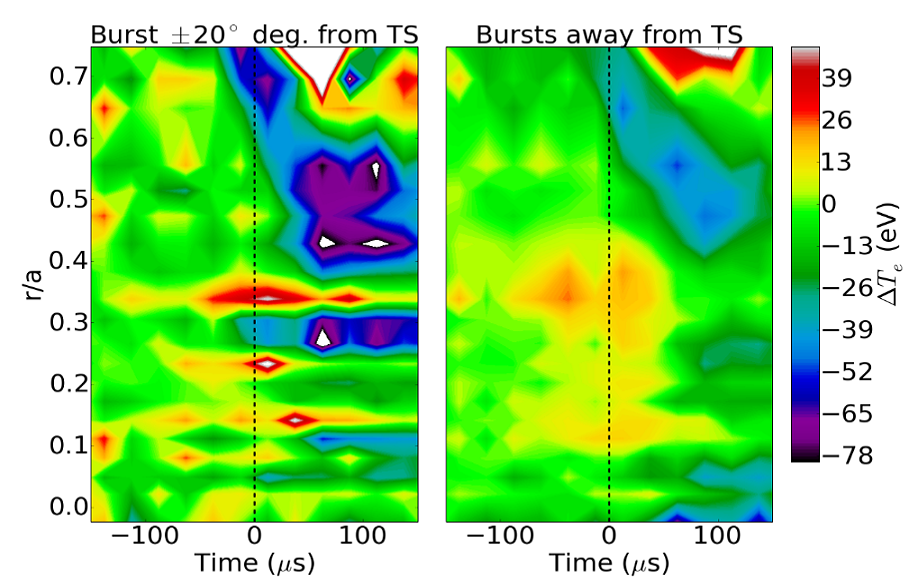
\includegraphics[width = 0.8\linewidth]{./m0_and_impurity_heating/m0_te_pulse.png}
	\caption[$T_e$ during $m = 0$ bursts]{$T_e$ measurement over an ensemble of $m = 0$ bursts showing a cold pulse-like feature traveling radially, as well comparatively small $T_e$ loss when the burst is away from the point of observation. (Reproduced from W. Young\cite{Young2015})}\label{fig:m0_te_pulse}
\end{figure}
\begin{figure}
	\centering
	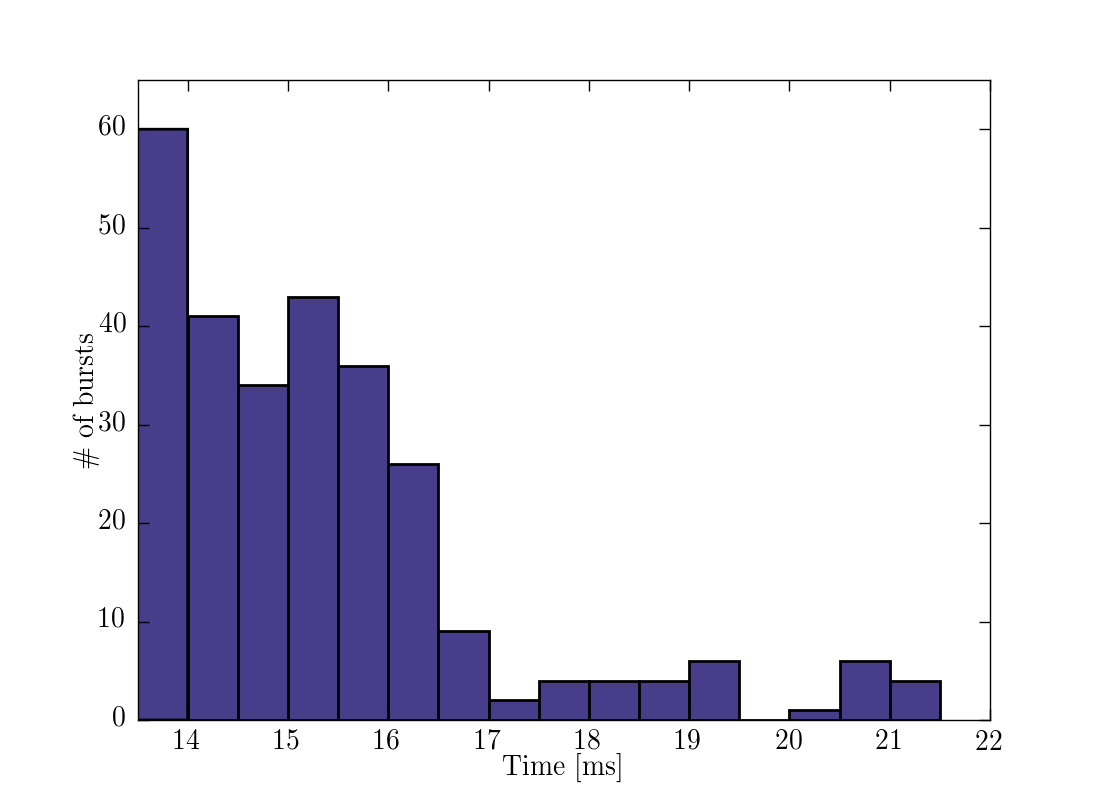
\includegraphics[width = 0.8\linewidth]{./m0_and_impurity_heating/m0_time_hist.png}
	\caption[Frequency histogram of $m = 0$ vs shot time]{Frequency histogram of $m = 0$ vs shot time. Note that the reversal of edge $E_\text{tor}$ is typically around 16ms in good PPCD. A bursty PPCD shot tends to have that delayed somewhat, but it is hard to quantify reliably.}\label{fig:m0_shot_time}
\end{figure}

\section{Observation of impurity heating associated with the $m = 0$ activities.}

The impurity temperature of C$^{6+}$ temperature are measured using CHERS at 50kHz and ensemble over similar events.
The dynamics being investigated occur at a faster timescale than the equlibration time between majority and impurity ions, and the CHERS measurements should not be interpreted as reflecting that of the majority. It is well known that sawtooth events heat the impurities more than the majority\cite{Magee2011}, and it is expected that the same applies to $m = 0$ burst heating.
% Cite Rich Magee's work here to support your statement:
%R.M. Magee, D. J. Den Hartog, S. T. A. Kumar, A. F. Almagri, B. E. Chapman, G. Fiksel, V. V. Mirnov, E. D. Mezonlin, J. B. Titus, Phys. Rev. Let 107, 065005 (2011).
Active CHERS measurement of C$^{6+}$ temperature show significant heating due to bursts radially located in the edge. Figure \ref{fig:m0_heating} shows the ensemble time evolution of the heating pulse for the range of measurement locations. The heating is very distinct in the edge locations but drops below regular fluctuation levels by chord 9 ($\rho/a = 0.37$). This is consistent with the expectation for $m = 0$ bursts which are localized at/near the reversal surface, and is similar to heating behavior of edge reconnection events examined by S. Gangadhara\cite{Gangadhara2008}. However, $T_i$ at the radial locations are observed to heat at the same time, and not display the radial delay seen in the $T_e$ measurements. Additionally, the temperature returns to equilibrium with a time scale $\lesssim 0.5ms$, which is significantly shorter than the expected ion confinement time. A comparison with the model's response to a burst-like event is presented in the next section.

\begin{figure}
	\centering
	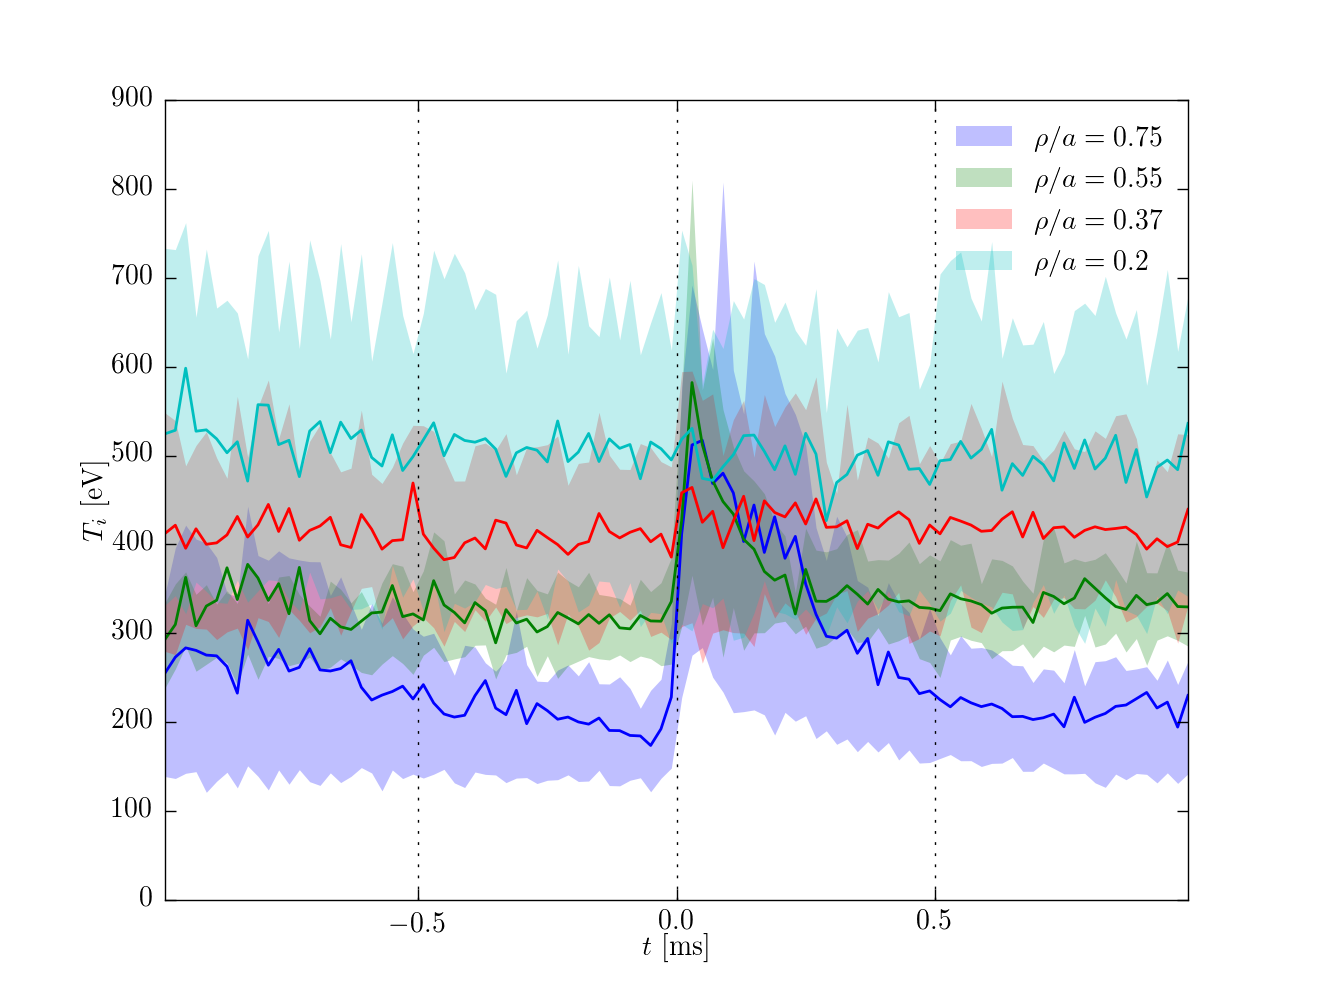
\includegraphics[width = 1.\linewidth]{./m0_and_impurity_heating/burst_heating_c6.png}
	\caption{Active CHERS measurement of C$^{6+}$ ensemble across bursts.}\label{fig:m0_heating}
\end{figure}

\begin{figure}
	\centering
	\includegraphics[width = 1.\linewidth]{./m0_and_impurity_heating/m0_no_delay.png}
	\caption{Ensemble $T_{C^{6+}}$ comparison between bursts toroidally near or far from the location of CHERS measurement ($\phi = 270^{\degree}$). Measurements are from $\rho/a = 0.75$. No indication of time delay associated with toroidal location.}\label{fig:m0_no_delay}
\end{figure}


An important observation resulting from the active measurements are high speed at which heating propagates around the machine. As can be seen in figure \ref{fig:m0_no_delay}, when the burst heating measurements are broken down into sub-ensembles separated by distance between the toroidal measurement location and the burst location, no delay is found. The charge exchange data is fitted at 50kHz, implying that any possible delay is smaller than 20$\mu s$. This indicates that the impurity heating is toroidally global. If we assume that the opposite is true, that the burst produces a local heating event located where the burst is located, then the toroidally local deposit of heat would need to travel to the other side of the device. For a very simple estimation of the time involved, the travel times of hypothetical deuterium ions at thermal velocity along equilibrium field line from one location to the direct opposite side of device toroidally are calculated for a range of $\rho$ near the reversal surface. This is presented in figure \ref{fig:heat_travel_time}. The actual thermal conduction time would be significantly longer than this as parallel conduction is slowed by collisions, and impurity thermal velocity is slower than deuterium. The delay of a toroially travelling heat pulse would be slower than 20$\mu s$, meaning that the observed heating is not a result of such a heat pulse, but the energy released through the $m = 0$ bursts travels around the device as EM waves/fluctuations and result in toroidally global (but radially local) impurity heating. The heating mechanism is not clear from this observation alone, however, informed speculation would posit that the $m = 0$ burst excites plasma waves and fluctuations that travel around toridally faster than ions can, and then heats the ions on the other side. Indeed, in Piovesan's prior work, $m = 1$ fluctuations are observed to be excited by $m = 0$ bursts, and propagate toroidally\cite{Piovesan2008}. The particulars of how that fluctuation leads to heating is likely complex and would be up for debate, considering that prior studies concluded that $m = 1$ fluctuations do not lead to heating if there is no accompanying $m = 0$ fluctuation. Mode coupling is likely involved, but there is insufficient evidence from observations made in this study.

\begin{figure}
	\centering
	\includegraphics[width = 1.\linewidth]{./m0_and_impurity_heating/m0_transit_time.png}
	\caption[Estimated carbon thermal transit time]{Estimated carbon thermal transit time. It is evaluated for hypothetical 400eV carbon ions at thermal velocity along equilibrium field line from one location to the direct opposite side of device toroidally. The dashed line labels $20 \mu s$ corresponding to the fitting frequency of 50kHz used for measurement data fitting.}\label{fig:heat_travel_time}
\end{figure}

The impurity heating associated with sawtooth events are known to be anisotropic, and the potential anisotropy of $m = 0$ induced impurity heating is investigated through passive IDS observations of C$^{4+}$ and C$^{2+}$ temperatures. The density profile of these two carbon charge states have limited radial extent, forming an emission 'shell'. A passive IDS view directly across the shell captures the perpendicular, and in ideal conditions, a view directly tangential to the emission shell at the reversal surface would return the parallel temperature. In reality the passive measurements cannot be directly translated to perpendicular and parallel temperature, although it is sufficient to estimate anisotropy in past studies \cite{Magee2011,Magee2011a}. Two emission shells are measured for anisotropy estimation. The C$^{2+}$ emission shell is located far out in the edge, outside of the reversal surface (at ~46cm -> $\rho/a = 0.9$) and it is extensively studied by T. Nishizawa during his drift wave work \cite{Nishizawa2018, Nishizawa2018b}. The C$^{2+}$ ions also have a higher mass-to-charge ratio, which, according to theories developed for sawtooth crash heating, should correlate to more significant heating and anisotropy\cite{Fiksel2009,Tangri}. However, direct comparisons between the two on this basis is difficult as the emission shells' radial location is different sufficiently that they reflect significantly different plasma conditions. The C$^{4+}$ emission shell is somewhat broader but located around the reversal surface. The measurements are performed simultaneously, and thus, each burst in the ensemble contributes information on both ~$T_{\perp}$ and ~$T_{\parallel}$. The (approximately) parallel observation is taken from the inboard side of the device to reduce any effects from the increased wall interaction during the burst, which primarily interacts with the outboard limiter. The results displayed in figure~\ref{fig:m0_anisotropy} show confusing contradiction. While both sets of measurements show anisotropy, the 'direction' of anisotropy is conflicting. The C$^{4+}$ measurement shows $\Delta T_{\parallel} > \Delta T_{\perp}$, but the C$^{2+}$ measurement shows $\Delta T_{\perp} > \Delta T_{\parallel}$. Additionally, the observed anisotropic heating associated with sawtooth events have the perpendicular direction being the strongly heated one, corresponding to expectations for possible heating mechanisms such as stochastic heating, or ion cyclotron damping. The strong parallel heating observed here with C$^{4+}$ does not have a ready-made heating mechanism associated. However, these anisotropy arguments should be taken with a grain of salt as described above, as well as the fact that the emission shell location may move dramatically over the course of the observation period as sharp movements in flux surface and particle flux is expected for the burst. It would be more ideal to observe anisotropy through active CHERS measurement, but currently the CHERS toroidal view is not able to measure the radial region of interest. 

\begin{figure}
	\centering
	\includegraphics[width = 1.\linewidth]{./m0_and_impurity_heating/m0_anisotropy.png}
	\caption[Anisotropic impurity heating associated with $m = 0$.]{Anisotropic impurity heating associated with $m = 0$. Approximately perpendicular and parallel temperatures are measured by taking advantage of the emission shell geometry. Results are presented for A) C$^{2+}$ and B)  C$^{4+}$}\label{fig:m0_anisotropy}
\end{figure}

\section{Classical ion thermal model results of $m = 0$ bursts}\label{sec:m0_v_model}

It is interesting to examine the equilibrium ion transport model response to a $m = 0$ -like heating event, through it is importantly to note that the model does not produce a direct comparison to observations as the model produces the response to direct majority ion heating. The zeroth order approximation involves simulating the burst heating by increasing the the \textit{ad hoc} term described in section \ref{sec:anomalous_heating} for a short duration (0.1ms) that corresponds to the typical burst duration. The magnitude of this increase is matched to the observed peak temperature at $\rho/a = 0.75$, and the model predictions are shown in figure \ref{fig:m0_model}. The characteristic time of the return to equilibrium as predicted by the forward model is noticeably longer than observations, especially for the $\rho/a = 0.55$ measurement location. This is despite the effect of the burst-induced temperature profile causing more heat loss in the edge region, due to both charge exchange, and particle loss. This discrepancy between the model and observation indicts one of the following:

\begin{itemize}
    \item The assumption that, except for the ion heating, the plasma is otherwise not meaningfully disturbed by the $m = 0$ burst is incorrect. Thus, additional transport mechanisms are 'activated' during the burst, and persist long enough to dissipate a significant portion of the heating. From previous discussion, we know that $T_e$ is significantly impacted by bursts, and FIR interferometry show that the bursts often lead to a sudden density drop followed by recovery. These would likely impact the plasma in significant ways that is not accounted for by this simple model estimation.
    %It would be good to think of a couple examples in anticipation of questions during your oral defense.
    \item The heating of the majority ions are significantly smaller than that of the impurities, and the burst measurements does not reflect the majority temperature evolution. Assuming that $m = 0$ related impurity heating is through similar mechanisms to that present in sawtooth crashes, then it would be expected that the impurities experience more heating than the majority ions. If this is the case, the observed T$_{C^{6+}}$ fall off would be determined primarily by the equilibration time with the majority ion, which is calculated to be ~0.3-0.5ms near the reversal surface for these plasma conditions. The observed equilibration time matches this time scale, but without direct measurements of $T_{D^+}$ the hypothesis cannot be confirmed.
    \item The model is deficient in complex and difficult to characterize ways.
\end{itemize}

\begin{figure}
	\centering
	\includegraphics[width = 1.\linewidth]{./m0_and_impurity_heating/m0_model.png}
	\caption[Model response to $m = 0$ like heating to the majority ions.]{Model response to $m = 0$ like heating to the majority ions. The model input data is the same shot ensemble used for analysis in the previous chapter, with the exception of a short burst of extra \textit{ad hoc} heating. }\label{fig:m0_model}
\end{figure}

It should be noted that the heating response produced is radially located to the same locations as observations without additional adjustments to the radial profile of the \textit{ad hoc} heating term. Considering the fact that the tearing mode activity is reduced and not eliminated, it is tempting to speculate that the \textit{ad hoc} heating needed by the model during the temperature share parallels in terms of mechanism to the heating seen during m = 0 bursts.
%The sentence above is an incomplete sentence. What are you speculating about the ad hoc heating term?

\section{Summary}

The impurity heating associated with $m = 0$ bursts are measured and investigated. Building upon prior understanding of $m = 0$ bursts, edge localized heating of carbon impurities are observed for $\rho/a \geq 0.55$. No signs of radial or toroidal propagation delay is observed at the time resolution available, indicating that the energy associated like traveled as waves and fluctuations and heats the relevant volume effectively simultaneously. Attempts to asses the anisotorpy of the heating is inconclusive, with the nature of emission shells and passive spectroscopy limiting our ability to interpret the measurements. Detailed modeling and understanding of plasma conditions and emission shell location shifts during a burst event may lead to better understanding of the passive measurements. A simple mock-up model calculation is constructed as a comparison. The model predicts that (if heated like impurities) the majority ions would retain the elevated temperature better than the measurement of carbon would indicate. This is likely due to a combination of over simplifying assumptions regarding background plasma conditions, and that majority ions behavior during a burst is likely different than that of the carbon impurities measured. 


\printbibliography%[title={Section bibliography}]
\end{refsection}

\begin{refsection}


\chapter{Conclusions and remarks}

\section{Summary of results}

A modeling approach is used to characterize ion thermal transport in improved confinement, reduced tearing (PPCD) plasmas in MST. The forward model is constructed in 1-D approximation and includes classical transport physics, charge exchange and particle flow. The model uses a range of diagnostic inputs to provide the plasma profiles (of $T_e$, $n_e$,$n_D$ as well as reconstructed magnetic) to predict $T_i$ evolution from an initial condition. This model is compared to measurement and found to be sufficient in predicting the core temperature evolution, but needed an \adhoc heating source localized in the gradient region to match observations. Additional thermal transport is not required to match measurements. The model includes the calculation of electron-ion equilibration, classical conduction, charge exchange loss, and flow related heating (including compression and convective heat flow). The model is applied to an ensemble of selected 500kA PPCD shots in MST, and it's temperature predictions are compared to measurements of $T_{C^{6+}}$ as a proxy of $T_i$.

The neutral dynamics is found to be important in constructing and analyzing the model. A physics based Monte Carlo simulation is used to calculate the neutral density and charge exchange loss, especially in the core. The simulations show that the core neutrals are 'warm' ($\approx 0.6-0.8 T_i$) and the charge exchange loss profile is hollow. Further, a portion of the energy lost to the neutrals is recovered via subsequent re-ionization. This simulation also provides the ionization source rate profile, which when combined with density measurements show that an inward particle flux in the core is necessary to account for the core density rise early in PPCD. Comparison is made with estimates of \ecb flux in PPCD and found to be a match. The compression effect of this flux is incorporated into the model, as well as the effect of the edge particle outflow. 

%Mark's email comments
%Make sure to list all of the unique things that you can point to which you did in your conclusion chapter. Keep in mind that you have done the most thorough analysis of ion heat transport in PPCD plasmas to date. You’ve done the most thorough analysis of neutral density profile evolution during PPCD which informs not only your ion power balance work, but has also been important in predicting charge state distributions of highly charge ions (like Aluminum) for predicting x-ray emission spectra (Patrick & Lisa’s work for the ME-SXR model and now the LLNL x-ray calorimeter). You’ve shown that any heating beyond classical mechanisms that you’ve called out in your model are edge localized. Your analysis of the m=0 burst activity also suggests that burst heating of the impurities may follow the same type of collisional equilibration with the deuterium that describes the ion heating due to magnetic reconnection present during edge-localized tearing mode excitation in standard plasmas.
%---

An \adhoc heating term is added to the model to match observations. The needed \adhoc term is located near the edge in the gradient region

The model's ion confinement time is found to be , and the largest loss mechanisms are found to be associated with particle loss out of the plasma, with charge exchange a near second. 

The phenomenon of impurity heating associated with m = 0 bursts in PPCD is investigated and found to have interesting properties such as edge locality, (near) simultaneous heating regardless of toroidal or radial location (except where there is no heating), and a faster than expected equilibration time. However, there are still many unclear aspects that surrounds this phenomenon that needs further investigation to clear up. 


This works presents the most thorough accounting for ion thermal transport in PPCD plasmas, and 



\section{Future work}
A more detailed assessment of turbulent heating mechanisms available 
Rutherford scattering measurements of D+ temperature, especially during the 
Direct measurements of neutral temperature. 


\printbibliography
\end{refsection}


% \include{related/related}

%% etc, etc.

%% Do you have appendices?  If so, add them here, just like chapters.
\begin{appendices}
% \include{backmatter/appendix1}
\chapter{Notes on terminology and notation}\label{app:term}
\begin{refsection}


I have often been confused by the question of terminology and notation in physics, and I suspect that this work of mine is not the exception as far as confusing terminology is concerned. In this work I try to keep the notation consistent and as much as possible, only assign one 'meaning' to any letter. Unfortunately, between the latin and Greek alphabets are only so long, and Chinese characters are not generally accepted in equations. In this appendix layout a reference for notation of various physics parameters, as well as discussion of potentially confusing terminology.

Starting with a table of notation for basic plasma parameters,
\begin{center}\begin{tabular}{p{1in}|p{3.5in}}
     $N$ &  Index of refraction\\ \hline
     $n$ & Density, subscripts e and i denotes electron and majority ion respectively\\ \hline
     $T$ & Temperature, subscripts same as $n$\\ \hline
     $t$ & Time\\ \hline
     $E, B$ & Electric and Magnetic field respectively\\ \hline
     $P$ & Thermal power (work) density\\ \hline
     $p$ & Plasma pressure\\ \hline
     $r$ & Minor radius \\ \hline
     $\rho, \rho_v$ & Volume average minor radius to the magnetic axis of a given flux surface, see section \ref{app:rhov}\\ \hline
     $q$ & Safety factor \\ \hline
     $Q$ & Heat flux \\ \hline
     $<\sigma v>$ & Average reaction rate assuming Maxwellian distribution\\ \hline
     $S$ & (Ion or electron) source rate per volume\\ \hline
     $\kappa$ & Thermal conduction coefficient, $=n\chi$\\
\end{tabular}\end{center}



\section{Power terms}\label{app_sec:power_terms}

As this is thesis deals with thermal transport modeling, thermal power terms are pervasive. Unless otherwise stated, these terms are power densities $P = 3/2nk_b \frac{\partial}{\partial t}T$ in units of [$W/m^3$], and the subscript describes the type of mechanism. Similarly, unless otherwise specified, the power terms refer to power flow into the majority ion species as positive. So broadly speaking, heating terms have $P > 0$ and loss terms have $P < 0$.

There is the additional consideration for mechanisms that affect the ion density and thermal energy at the same time. This includes all the mechanisms that affects density, as any given 'new' population of ions will have a certain amount of thermal energy associated with it. A good example of this is the electron impact ionization of neutrals. As stated in section\ref{sec:neutral_physics}, the electron impact ionization of warm neutrals represents a net gain of thermal energy, but it also represents a density source term. Since these neutrals typically have a temperature less than $T_i$, the process cools the plasma despite representing a gain of thermal energy. The ionization of neutrals are better thought of as a gain of pressure. These power terms do not obey the power to temperature related above. Instead:
\begin{align}
    P &= 3/2k_b \frac{\partial}{\partial t}(n T) \\
    \frac{2P}{3k_b} &= T\partialt n + n \partialt T \\
    \partialt T &= \frac{2P}{3k_b} - T\partialt n 
\end{align}

Note that does not directly reflect how these values are calculated in the code, as the figure of merit being calculated and saved by the code is total thermal energy and not temperature. The temperature is only calculated afterwards for comparison to measurement. 

The following is a table of the power density term and their meaning,
\begin{center}\begin{tabular}{p{1in}|p{3.5in}}
$P_{\text{eq}}$ & Electron ion equilibration power, see section \ref{sec:equilibration_power}\\ \hline
$P_{\text{cond}}$ & Classical thermal conduction power, see section \ref{sec:thermal_cond}\\ \hline
$P_{\text{CX}}$ & Net charge exchange 'transport', $= P_{\text{CX loss}}+P_{\text{e-imp}}$, see section \ref{sec:neutral_physics}\\ \hline
$P_{\text{CX loss}}$ & Charge exchange loss, see section \ref{sec:neutral_physics}\\ \hline
$P_{\text{e-imp}}$ & Power from electron impact ionization of hot neutrals, see section \ref{sec:neutral_physics}\\ \hline
$P_{\text{flow}}$ & Total flow power, $=P_{\text{flow cons}} + P_{\text{comp work}}$, see section \ref{sec:flow_effects}\\ \hline
$P_{\text{flow cons}}$ & Flow conservation power, see section \ref{sec:flow_effects}\\ \hline
$P_{\text{comp work}}$ & Compressional work from \ecb pinch, see section \ref{sec:flow_effects} and \ref{sec:eb_pinch}\\ \hline
$P_{\text{neo}}$ & Neoclassical thermal conduction.\\ \hline
%$P_{\text{anomalous}}$ & anomalous thermal power, including heating, cooling and transport\\
$P_{\textit{ad hoc}}$ & \adhoc heating power, used in the model to match edge observations, see section \ref{sec:anomalous_heating}\\


\end{tabular}\end{center}


\section{Relating to charge exchange spectroscopy}

A brief but important note on terminology regarding charge exchange measurements. Consider the case where a $C^{6+}$ ion charge exchanges with a neutral, thus gaining an electron and becoming $C^{5+}$, but immediately emits a photon as the electron de-excites. The observations made through this process would reflect the temperature, velocity, and density of the $C^{6+}$ charge state. However, the emission line is the same as if an $C^{5+}$ ion undergoes electron impact excitation, referred to as a CVI emission line. Hence, when talking about a specific emission line and how it relates to the spectrometer, the Roman numeral notation (eg, 343nm CVI line) is used. Otherwise, the text will refer to the particular ion charge state being measured (eg, $C^{6+}$ or $C^{5+}$), whenever relevant, it will also be specified if the measurement made is 'active', that is localized and through CHERS, or 'passive', that is through ion Doppler spectroscopy. 

Further, there is the minor distinction made in this these between ion Doppler spectroscopy (IDS): the set of physical process and principles described in section \ref{sec:ids}, and the Ion Doppler Spectrometer mk. I and mk. II (IDS-I and IDS-II): the physical spectrometers used at MST for both passive IDS measurements and active CHERS measurements.

\section{The radial coordinate $\rho_v$}\label{app:rhov}

The radial coordinate used for the modeling in this work is is $\rho_v$ as opposed to the more straight forward minor radius r. $\rho_v$ is, approximately, the radius of the relevant flux surface, since flux surfaces in axisymmetric MST plasmas are nearly perfect circles. Alternatively, it is equivalent to the volume average minor radius to the magnetic axis. This radial coordinate is defined and calculated by MSTfit\cite{Anderson2001}. It is chosen over the minor radius r as the radial coordinate for two reasons. Firstly, it better accounts for the fact that the flux surfaces are Shafronov-shifted outwards by a varying amount, and secondly, existing code important to this modeling work, in particular MSTfit, uses $\rho_v$ as it's radial coordinates. However, in these PPCD plasmas the ultimately difference between r and $\rho_v$ is small, especially in terms of $r/a$ vs $\rho_v/a$, typically within or close to the radial position uncertainty of any given diagnostic measurement. This is the reason why the impurity levels taken from M. Nornberg's paper\cite{Nornberg2018} is incorporated on a $\frac{r}{a}\approx\frac{\rho_v}{a}$ basis, instead of redoing the analysis in the shifted coordinate. 


\printbibliography
\end{refsection}
\chapter{Coding structure, techniques, and considerations}\label{app:code}

This appendix serves as a discussion of the methods (and reasons why) the code uses to propagate the model on two different time scales, of the code structure, of methods to enforce pseudo-self-consistency using predictor corrector methods, as well as mathematical and coding considerations relating to the modeling code. This appendix serves as a guide for any scientist who likes to understand the details of the model construction, possibly to improve or adjust it's function. For a more user friendly manual on how to use the code and how to interpret the results, see Appendix \ref{app:manual}. Unless otherwise mentioned, all the codes discussed in this section are in IDL.




The setup is performed by the function called analyze\_set(). It's purpose it quite simple: to automate the generation of input files as well as the analysis of a set of plasma shots, either as an ensemble, or as a list of individual shots. Even thought it's structure was made for ensemble analysis, it can also process a list of a single shot, essentially automating the single shot analysis procedure as well. As the code was written primarily to enable ensembling analysis, that is the view point I will take in describing the structure. Single shot analysis is enabled by treating it as an ensemble of one shot. 

The setup first determines time block  division of the analysis period. Then, it reads data from the MDSplus tree into IDL as MST\_signal objects by hijacking the data acquisition routines in MSTfit. The object structure provides the data handling capabilities such as truncating the data to desired segments and ensemble averaging across the same signal from several shots. Then for each time block, the code generates a *.mst file that is required by MSTfit, using the same methods used by MSTfit itself, but instead of taking the data direction from MDSplus, the code uses the signal objects.
\chapter{User manual for ion transport code}\label{app:manual}

This appendix is written for the scientists who would wish to use the code to produce calculations and predictions without examining the belly of the beast as far as how the code is running. If you are looking for details on how the code works and why it's set up the way it is, please refer to Appendix \ref{app:code}.

    
\end{appendices}



%% McBride is a very nice style (some version is included in this distribution)
%\bibliographystyle{unsrt}


%% Want an index?  Neither did I.
%\printindex

\end{document}
